% Copyright (C) 2014-2017 by Thomas Auzinger <thomas@auzinger.name>

\documentclass[draft,final]{vutinfth} % Remove option 'final' to obtain debug information.

% Load packages to allow in- and output of non-ASCII characters.
\usepackage{lmodern}        % Use an extension of the original Computer Modern font to minimize the use of bitmapped letters.
\usepackage[T1]{fontenc}    % Determines font encoding of the output. Font packages have to be included before this line.
\usepackage[utf8]{inputenc} % Determines encoding of the input. All input files have to use UTF8 encoding.

% Extended LaTeX functionality is enables by including packages with \usepackage{...}.
\usepackage{amsmath}    % Extended typesetting of mathematical expression.
\usepackage{amssymb}    % Provides a multitude of mathematical symbols.
\usepackage{mathtools}  % Further extensions of mathematical typesetting.
\usepackage{microtype}  % Small-scale typographic enhancements.
\usepackage[inline]{enumitem} % User control over the layout of lists (itemize, enumerate, description).
\usepackage{multirow}   % Allows table elements to span several rows.
\usepackage{booktabs}   % Improves the typesettings of tables.
\usepackage{subcaption} % Allows the use of subfigures and enables their referencing.
\usepackage[ruled,linesnumbered,algochapter]{algorithm2e} % Enables the writing of pseudo code.
\usepackage[usenames,dvipsnames,table]{xcolor} % Allows the definition and use of colors. This package has to be included before tikz.
\usepackage{nag}       % Issues warnings when best practices in writing LaTeX documents are violated.
\usepackage{todonotes} % Provides tooltip-like todo notes.
\usepackage{hyperref}  % Enables cross linking in the electronic document version. This package has to be included second to last.
\usepackage[acronym,toc]{glossaries} % Enables the generation of glossaries and lists fo acronyms. This package has to be included last.

% Define convenience functions to use the author name and the thesis title in the PDF document properties.
\newcommand{\authorname}{Tom Tucek} % The author name without titles.
\newcommand{\thesistitle}{INTRA SPACE Agent} % The title of the thesis. The English version should be used, if it exists.

\usepackage{catoptions}
\makeatletter
\def\figureautorefname{figure}
\def\tableautorefname{table}
\def\Autoref#1{%
  \begingroup
  \edef\reserved@a{\cpttrimspaces{#1}}%
  \ifcsndefTF{r@#1}{%
    \xaftercsname{\expandafter\testreftype\@fourthoffive}
      {r@\reserved@a}.\\{#1}%
  }{%
    \ref{#1}%
  }%
  \endgroup
}
\def\testreftype#1.#2\\#3{%
  \ifcsndefTF{#1autorefname}{%
    \def\reserved@a##1##2\@nil{%
      \uppercase{\def\ref@name{##1}}%
      \csn@edef{#1autorefname}{\ref@name##2}%
      \autoref{#3}%
    }%
    \reserved@a#1\@nil
  }{%
    \autoref{#3}%
  }%
}
\makeatother

% Set PDF document properties
\hypersetup{
    pdfpagelayout   = TwoPageRight,           % How the document is shown in PDF viewers (optional).
    linkbordercolor = {Melon},                % The color of the borders of boxes around crosslinks (optional).
    pdfauthor       = {\authorname},          % The author's name in the document properties (optional).
    pdftitle        = {\thesistitle},         % The document's title in the document properties (optional).
    pdfsubject      = {Subject},              % The document's subject in the document properties (optional).
    pdfkeywords     = {a, list, of, keywords} % The document's keywords in the document properties (optional).
}

\setpnumwidth{2.5em}        % Avoid overfull hboxes in the table of contents (see memoir manual).
\setsecnumdepth{subsection} % Enumerate subsections.

\nonzeroparskip             % Create space between paragraphs (optional).
\setlength{\parindent}{0pt} % Remove paragraph identation (optional).

\makeindex      % Use an optional index.
\makeglossaries % Use an optional glossary.
%\glstocfalse   % Remove the glossaries from the table of contents.

% Set persons with 4 arguments:
%  {title before name}{name}{title after name}{gender}
%  where both titles are optional (i.e. can be given as empty brackets {}).
\setauthor{}{\authorname}{}{male}
\setadvisor{Associate Prof. Dipl.-Ing. Dipl.-Ing. Dr.techn.}{Michael Wimmer}{}{male}


% For bachelor and master theses:
\setfirstassistant{Projektass. (FWF) Dipl.-Ing. }{Christian Freude}{BSc}{male}
%\setsecondassistant{Pretitle}{Forename Surname}{Posttitle}{male}
%\setthirdassistant{Pretitle}{Forename Surname}{Posttitle}{male}


% For dissertations:
%\setfirstreviewer{Pretitle}{Forename Surname}{Posttitle}{male}
%\setsecondreviewer{Pretitle}{Forename Surname}{Posttitle}{male}

% For dissertations at the PhD School and optionally for dissertations:
%\setsecondadvisor{Pretitle}{Forename Surname}{Posttitle}{male} % Comment to remove.

% Required data.
\setaddress{Kanalstrasse 8/2; 1220 Vienna; Austria}
\setregnumber{01325775}
\setdate{29}{11}{2018} % Set date with 3 arguments: {day}{month}{year}.
\settitle{\thesistitle}{INTRA SPACE Agent} % Sets English and German version of the title (both can be English or German). If your title contains commas, enclose it with additional curvy brackets (i.e., {{your title}}) or define it as a macro as done with \thesistitle.
\setsubtitle{An Agent-Based Architecture for an Artistic Real-Time Installation}{An Agent-Based Architecture for an Artistic Real-Time Installation} % Sets English and German version of the subtitle (both can be English or German).

% Select the thesis type: bachelor / master / doctor / phd-school.
% Bachelor:
\setthesis{bachelor}
%
% Master:
%\setthesis{master}
%\setmasterdegree{dipl.} % dipl. / rer.nat. / rer.soc.oec. / master
%
% Doctor:
%\setthesis{doctor}
%\setdoctordegree{rer.soc.oec.}% rer.nat. / techn. / rer.soc.oec.
%
% Doctor at the PhD School
%\setthesis{phd-school} % Deactivate non-English title pages (see below)

% For bachelor and master:
\setcurriculum{Media Informatics and Visual Computing}{Medieninformatik und Visual Computing} % Sets the English and German name of the curriculum.

% For dissertations at the PhD School:
%\setfirstreviewerdata{Affiliation, Country}
%\setsecondreviewerdata{Affiliation, Country}

\usepackage{listings}
\usepackage{color}

\definecolor{dkgreen}{rgb}{0,0.6,0}
\definecolor{gray}{rgb}{0.5,0.5,0.5}
\definecolor{mauve}{rgb}{0.58,0,0.82}

\lstset{frame=tb,
	language=Java,
	aboveskip=3mm,
	belowskip=3mm,
	showstringspaces=false,
	columns=flexible,
	basicstyle={\small\ttfamily},
	numbers=none,
	numberstyle=\tiny\color{gray},
	keywordstyle=\color{blue},
	commentstyle=\color{dkgreen},
	stringstyle=\color{mauve},
	breaklines=true,
	breakatwhitespace=true,
	tabsize=3
}


\begin{document}

\frontmatter % Switches to roman numbering.
% The structure of the thesis has to conform to
%  http://www.informatik.tuwien.ac.at/dekanat

\glsunsetall

\addtitlepage{naustrian} % German title page (not for dissertations at the PhD School).
\addtitlepage{english} % English title page.

\glsresetall

\addstatementpage

\begin{danksagung*}

Ich möchte hiermit allen Projektmitgliedern von INTRA SPACE danken, welche mir erlaubten, mich an ihrem Streben nach Wissen zu beteiligen.
Mein besonderer Dank gilt dem Team innerhalb des Raumes in welchem alles stattfand – Christina Jauernik, Simon Oberhammer, Martin Perktold und Christian Freude. 
Letzterer, welcher mich nicht nur während der Entwicklung unterstützte, sondern auch mein Schreiben an dieser Arbeit mit konstruktiver Kritik und gütigem Beistand förderte, stellt einen der Hauptgründe dar, dass dieses Werk fertiggestellt wurde. \\
Ich möchte weiters sowohl Professor Wolfgang Tschapeller und Esther Balfe danken, wessen Wirken an diesem Projekt mich zu neuen Sichtweisen im Rahmen der Wissenschaft führte. 
Weiterer Dank gilt Professor Michael Wimmer, welcher mir die Gelegenheit bat, an diesem Projekt zu arbeiten und diese Arbeit an seinem Institut zu schreiben. \\
Danke an Professor Michael Thielscher, welcher unserem Team dabei half, mit Agenten Entwicklung anzufangen und uns den Weg geleitete. 
Ich bin besonders dankbar für die Unterstützung durch Professor Paolo Petta, welcher uns alle ermutigte und inspirierte, neue Wege zu finden, selbst wenn unser Team nicht weiter wusste. \\
Schließlich möchte ich all meinen Freunden, meiner Familie und meinem Hund danken – für all ihren konstanten Beistand und ihre Ermutigung im Laufe meiner Arbeit.
Spezieller Dank gilt meinem Vater, für seine stetige Bereitschaft mich in allem zu unterstützen was ich unternehme.

\end{danksagung*}

\begin{acknowledgements*}

I would like to express my gratitude to the entire team of project INTRA SPACE, who allowed me to join them in their pursuit of knowledge. 
Special thanks go out to the team stationed inside of the development room, consisting of Christina Jauernik, Simon Oberhammer, Martin Perktold, and Christian Freude. 
The latter, who did not only aid me during project development, but also supported me in writing this work with both wisdom and patience, giving constructive criticism and benevolent assistance, was a major cause for this thesis to be finished. \\
Further thanks to both Professor Wolfgang Tschapeller and Esther Balfe, whose work on this project opened my eyes to new ways of thinking in an academic setting. 
I would also like to thank Professor Michael Wimmer, who allowed me to work on this project and write this thesis at his institute. \\
Thanks to Professor Michael Thielscher, for helping the project team getting started with agent development and guiding us on our way. 
I am particularly grateful for the assistance given by Professor Paolo Petta, for encouraging and inspiring our team in times we had trouble finding ways to advance. \\
Finally, I wish to thank all of my friends, my family and my dog, for their support and encouragement throughout my work. 
Special thanks to my father, for his constant willingness to assist me in everything I do.

\end{acknowledgements*}

\begin{kurzfassung}

Diese Arbeit behandelt und beschreibt die Entwicklung und Einbettung eines Agenten-Systems in eine künstlerische Einrichtung. 
Das System ist dafür verantwortlich, virtuelle Figuren auf einer Leinwand zu kontrollieren, um somit Besuchern der Einrichtung die Interaktion mit jenen Figuren zu ermöglichen. 
Das Benehmen der Agenten basiert auf zuvor vom Projekt-Team gestalteten Stories und soll darauf optimiert sein, sowohl gut von Besuchern aufgefasst zu werden, als auch dem Projekt Team zu erlauben, an der Interaktion zwischen Menschen und Nicht-Menschen zu forschen. \\
Die Implementierung des Agenten Systems wurde mittels Jason wahrgenommen, eines Java-basierten Interpreters der Agenten-Programmiersprache AgentSpeak. 
Es wurden unterschiedliche Agenten-Szenarien über den Verlauf des Projektes entwickelt und mittels verschiedener Herangehensweisen implementiert. 
Ein iterativer und dynamischer Entwicklungsprozess wurde verfolgt, während regelmäßige Meetings der Projektmitglieder stattfanden, bei welchen Fortschritt und Ideen mit Unterstützung von Visualisierungen diskutiert wurden. 
Das Verhalten der Agenten war von vielen Problemen geprägt, da die Agenten entweder zu sehr von Reaktionen auf Besucherverhalten abhängig waren, oder sich stattdessen zu stark auf eigene Ziele konzentrierten, worunter die Qualität der Interaktion mit Besuchern der Einrichtung litt. 
Um diese Probleme zu lösen, wurden unterschiedlichste Ansätze verfolgt, diskutiert und dokumentiert.\\
In der finalen Version der Einrichtung wurden Agenten mit indeterministischem und emergentem Verhalten eingesetzt. 
Weiters haben Agenten den Fokus auf Besucherverhalten mit dem Verfolgen der eigenen Ziele balanciert, was zur Folge hatte, dass Besucher die Agenten als gesellschaftliche Präsenz wahrnehmen konnten, während die Interaktion auf sowohl natürliche, als auch neuartige Weise stattfinden konnte.

\end{kurzfassung}

\begin{abstract}

This work describes the processes involved in developing and embedding an agent system into an artistic real-time installation. 
The agent system would be responsible for controlling virtual figures on a screen, which interact with users of the installation. 
It was necessary to develop agents which displayed behavior pre-defined in stories designed by the project team, as well as to ensure that such agents acted in a way that was both well received by visitors, while also stimulating interaction in a way that allowed the project team to conduct research on the interactions between humans and nonhumans.\\
The agent system was implemented using Jason, a Java-based interpreter of the agent-programming language AgentSpeak. 
Over the course of the project, various agent scenarios were developed, with differing ways of implementation. 
An iterative process was used for development and regular meetings with project members were instated, to discuss progress and ideas, while utilizing visualizations to aid communication. 
Behavior of developed agents was plagued by various problems, from being too reliant on reactions towards user behavior, to not interacting enough with active users. Various approaches to such problems were tried out, discussed, and documented.\\
During the final installation, agents with indeterministic and emergent behavior were employed. 
Furthermore, agents were focused on both pursuing their own goals as well as constantly paying attention to visitor behavior. 
This allowed users to realize agents as a social presence and interact with them in a way that was both novel and natural. 

\end{abstract}

% Select the language of the thesis, e.g., english or naustrian.
\selectlanguage{english}

% Add a table of contents (toc).
\tableofcontents % Starred version, i.e., \tableofcontents*, removes the self-entry.

% Switch to arabic numbering and start the enumeration of chapters in the table of content.
\mainmatter

\newacronym{ia}{IA}{Intelligent Agent}
\newacronym{bson}{BSON}{Binary \gls{json}}
\newacronym{json}{JSON}{JavaScript Object Notation}
\newacronym{as}{AS}{AgentSpeak}
\newacronym{mas}{MAS}{Multi-agent system}
\newacronym{fwf}{FWF}{Fonds zur Förderung der wissenschaftlichen Forschung (Austrian Science Fund)}
\newacronym{ai}{AI}{Artificial Intelligence}
\newacronym{cartago}{CArtAgO}{Common ARTifact infrastructure for AGents Open environments}
\newacronym{fubi}{FUBI}{Full Body Interaction Framework}
\newacronym{bdi}{BDI}{Belief-Desire-Intention}
\newacronym{udp}{UDP}{User Datagram Protocol}

\newglossaryentry{agent figure}
{
  name={agent}{figure},
  text={agent}{figure},
  description={Also virtual agent-figure. Refers to the agent controlled figure on the screen}
}

\newglossaryentry{jason agent}
{
  name={Jason agent},
  description={The agent program controlling the \gls{agent figure}}
}

\newglossaryentry{visitor}
{
  name={Visitor},
  description={Active user of the INTRA SPACE installation}
}

\newglossaryentry{live}
{
  name={Live},
  description={Also live state or live phase. Refers to the state, in which the \gls{agent figure} mirrors the movements of the \gls{visitor} it was assigned to}
}

\newglossaryentry{island system}
{
  name={island-system},
  text={island-system},
  description={A concept similar to finite-state machines, used to visualize and model \glspl{jason agent}. Described more closely in \Autoref{chap:finalapproach}}
}


\chapter{Introduction}
\label{chap:introduction}

This work describes the process and challenges of developing an agent-based system for an artistic real-time installation called INTRA SPACE. 
The installation, which was being developed as an artistic research project by the academy of fine arts in Vienna in cooperation with the TU Wien, had the goal of exploring and deconstructing interactions between humans and so-called nonhumans. 
The main idea of the installation was to offer \glspl{visitor} the chance to interact with a virtual figure on a wide screen in front of them. 
The virtual figures would guide \glspl{visitor} through certain procedures, mimic them, interact with them, as well as follow their own goals. \\
The virtual figures were to be controlled by an independently running agent-system, which would have access to information regarding the \glspl{visitor}’ behavior, and should thus determine the actions of one or more characters on the screen. 
Furthermore, the agents’ course of action had been predefined by various stories, written by the research group. 
Converting these stories into \gls{as} using Jason was the first main goal of the task. Caused by the constantly developing environment of the project, development of the agent system faced various dynamic goals as well.
The research question of this work is thus “How can an agent system be developed and embedded into an installation with dynamic requirements?”. 
This document describes the project’s vision and set-up, followed by a detailed description of the process of developing, implementing, and embedding an agent system into the artistic real-time installation of the project. \\
This work is generally structured chronologically, as implementations are presented in the order they were developed. 
However, alternatives and other additional information are sometimes based more on hindsight and reflection. 
After the installation is described and explained, an overview of related works is presented as well. The aforementioned research question and resulting sub-questions are presented with multiple possible approaches, as well as detailed descriptions of the paths which were actually chosen and implemented. 
Concluding remarks include reflections on the project, problems, possible solutions and approaches, discussion, and further work.

\section{About Project INTRA SPACE}
\label{chap:about}

Project INTRA SPACE was an artistic research project by the academy of fine arts in Vienna, which ran from April 2015 until June 2017, with involvement of the author of this work starting in August 2016. 
It was funded by the \gls{fwf}.
\begin{quote}
	``\emph{INTRA SPACE: The reformulation of architectural space as a dialogical aesthetic} explores how interactions between, across and beyond humans and nonhumans can be experimentally embodied, aesthetically reformulated and theoretically challenged in their spatial, temporal and transversally entangled spheres.''~\cite{intraspaceAbout}
\end{quote}
\Glspl{visitor} were able to experience the finished product either by themselves, or watch performers interact with it. 
Although the installation was considered mobile and has been rebuilt at another location for presentation purposes, its development, testing, and presentation during the author’s involvement were conducted within a single room. 
The layout of the room was changed multiple times during development, with the final layout being presented as a schematic overview in Figure~\ref{fig:fig1_overview}, as well as a picture, taken from the screen’s side opposing the motion-capture space, in Figure~\ref{fig:fig2_installation}. \\
The layout seen in Figure~\ref{fig:fig1_overview} can be separated into a motion-capture space, a back-projection space, as well as two work spaces. 
Computers running necessary software or used for development were placed in the work spaces. 
The two most notable computers were called the “Render Node” and the “Captury Node”. 
First of which was connected to the projector and responsible for agents appearing on screen, as well as hosting the agent system. 
The second PC called “Captury Node” was connected to the cameras tracking the \gls{visitor} within the motion-capture space.
This machine was responsible for processing live picture data fed to it via Ethernet, discerning relevant information, such as the tracked person’s position and movements, and finally sending the pre-processed data to the “Render Node”. \\
The installation before the introduction of \gls{ai} was comparable to~\cite{10.1007/978-3-319-09767-1_7} with the agent on the screen mirroring the \gls{visitor}'s movements in real time. 
After a short “donning” phase (explained further in \Autoref{chap:donning}), the \gls{visitor}’s movements were entirely recreated by the \gls{agent figure} on the screen (see Figure~\ref{fig:fig3_action}). 
As seen in Figure~\ref{fig:fig2_installation} and Figure~\ref{fig:fig3_action}, \glspl{agent figure} were not rendered in a photorealistic way during the final phases of the project, but instead were chosen to be represented by monochromatic, sexually ambiguous models. 
There were several models in use, as can be seen in Figure~\ref{fig:fig4_models}, and a common characteristic was the high polygon count for the figures faces and hands, while their bodies were made of a noticeably lesser amount of polygons.\\
The goal of adding an agent system to the project was for the \gls{agent figure} to “emancipate” and disconnect from the \gls{visitor}, realizing its own motions and behavior, thus allowing, even provoking, more interaction between the \gls{visitor} and the figure. 
The initial vision consisted of the \gls{agent figure} copying the \gls{visitor}’s movements for a random, but limited amount of time, before slowly starting to act on its own. 
The \gls{visitor} was supposed to gradually realize the emancipation of the figure, and move on from one-way interaction by being replicated, to two-way interaction by gesture-based dialogue.
The agent system containing the required \gls{ai} initially had to meet the following requirements:
\begin{itemize}
	\item Communicate with the already installed system by sending and receiving information via a defined interface
	\item Run isolated and independently from the rendering engine, be fault tolerant and stable
	\item Take control over the \glspl{agent figure}’ actions at appropriate times
	\item Incorporate pre-written stories into interactions with \glspl{visitor}
	\item Make decisions based on the information it is presented in real time (information may be incomplete or faulty)
\end{itemize}
During development additional requirements emerged, such as non-deterministic behavior and \gls{visitor} guidance, which are further explored in later chapters. \\
Development of the agent system took place in a period of about six months, using iterations and continuous feedback from project staff, experts, and \glspl{visitor}. 
Implementation was based on independent stories, which were to be told by the \glspl{agent figure}’ actions. 
Stories would sometimes feature branching paths depending on \gls{visitor} behavior, or would not follow a time line at all, but rather be purely reactive in nature. 
Early agent stories were mostly based either on animalistic behavior, such as that of a bat or an octopus, or on goals to be reached – for example getting the \gls{visitor} to perform a certain action, such as waving towards the agent. 
Some of the stories are explained in detail in \Autoref{chap:implementation}. \\
Pre-recorded motions from the motion-capture software The Captury Live~\cite{capturyLive} were used as basic building blocks for agent behaviour. 
These motions could either be of continuous nature, such as walking or standing animation cycles, or isolated actions, such as hand gestures. 
Certain actions would leave the agent in a different state then before. 
For example, sitting down on the floor or getting up, would switch between the states of standing and sitting, thus enabling the agent to perform different actions from before. 
Because of graphic depictions of such features, stories for the agent system eventually transformed into state machines – a topic which is further discussed in \Autoref{chap:sleeper}.
\begin{figure}[h]
	\centering
	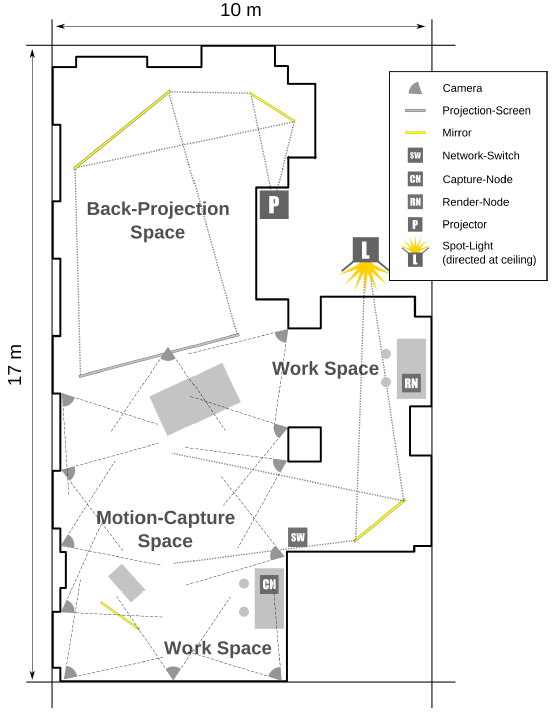
\includegraphics[width=\textwidth]{fig1_overview}
	\caption{Schematic plan of final setup. (Taken from the technical report about INTRA SPACE, by Christian Freude.)}
	\label{fig:fig1_overview}
\end{figure}
\begin{figure}[h]
	\centering
	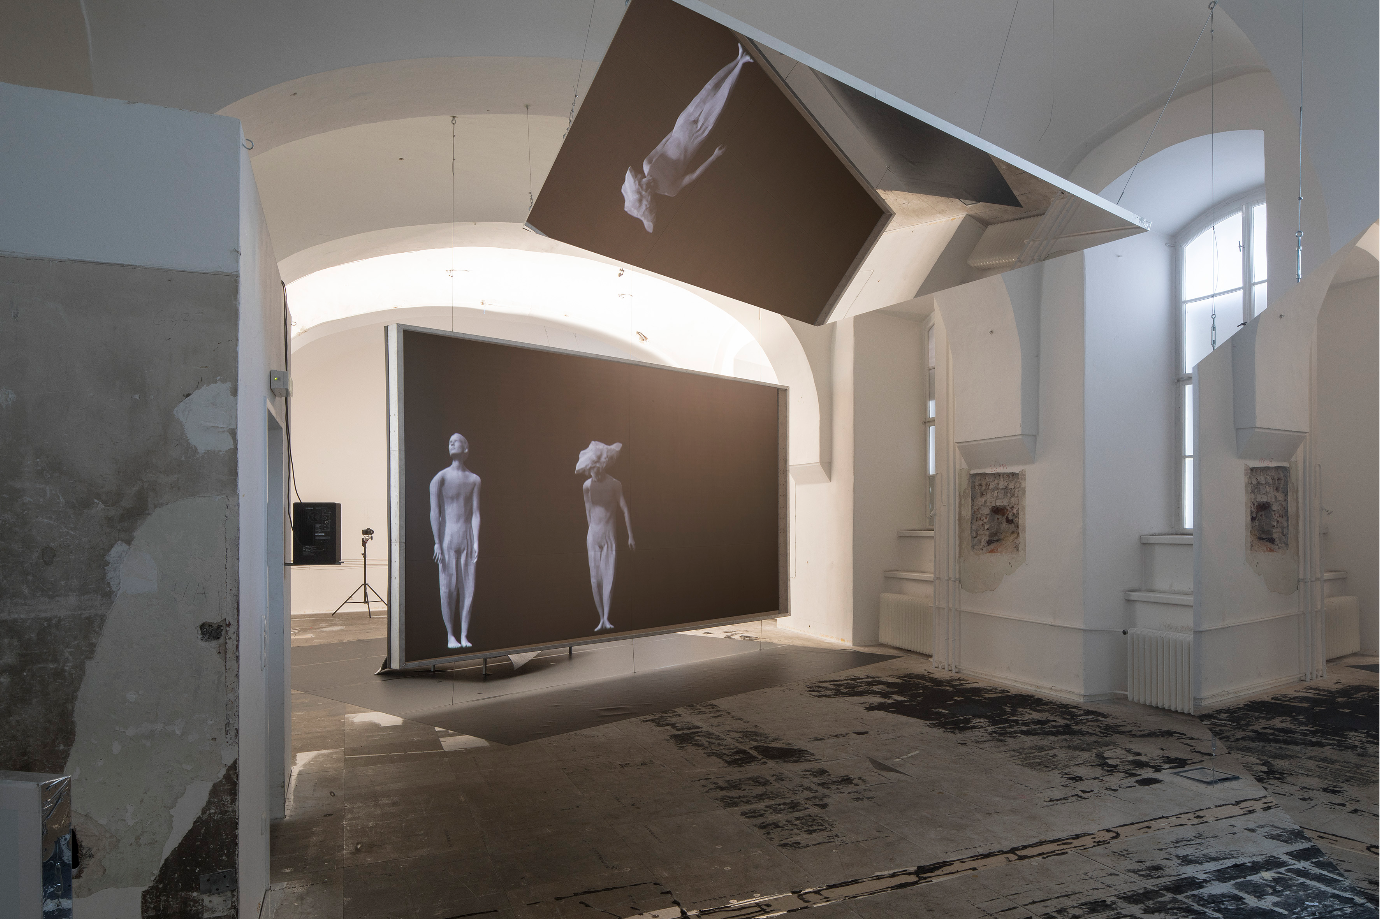
\includegraphics[width=\textwidth]{fig2}
	\caption{Picture of the installation. (Picture taken by Günter Richard Wett.)}
	\label{fig:fig2_installation}
\end{figure}
\begin{figure}[h]
	\centering
	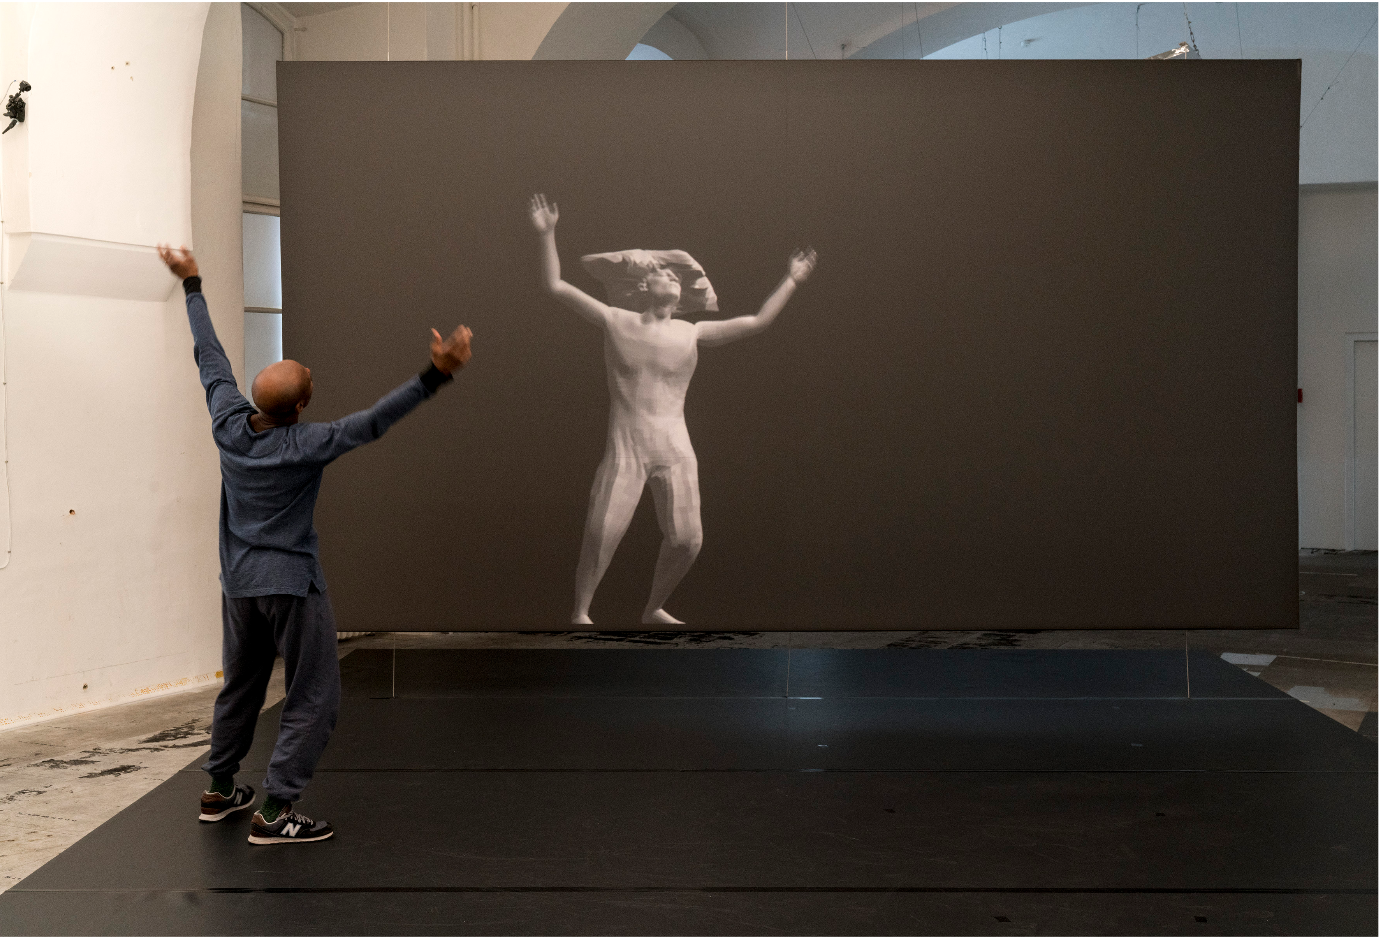
\includegraphics[width=\textwidth]{fig3}
	\caption{Picture of the \gls{agent figure} mirroring the \gls{visitor}’s movements. (Picture taken by Günter Richard Wett.)}
	\label{fig:fig3_action}
\end{figure}
\begin{figure}[h]
	\centering
	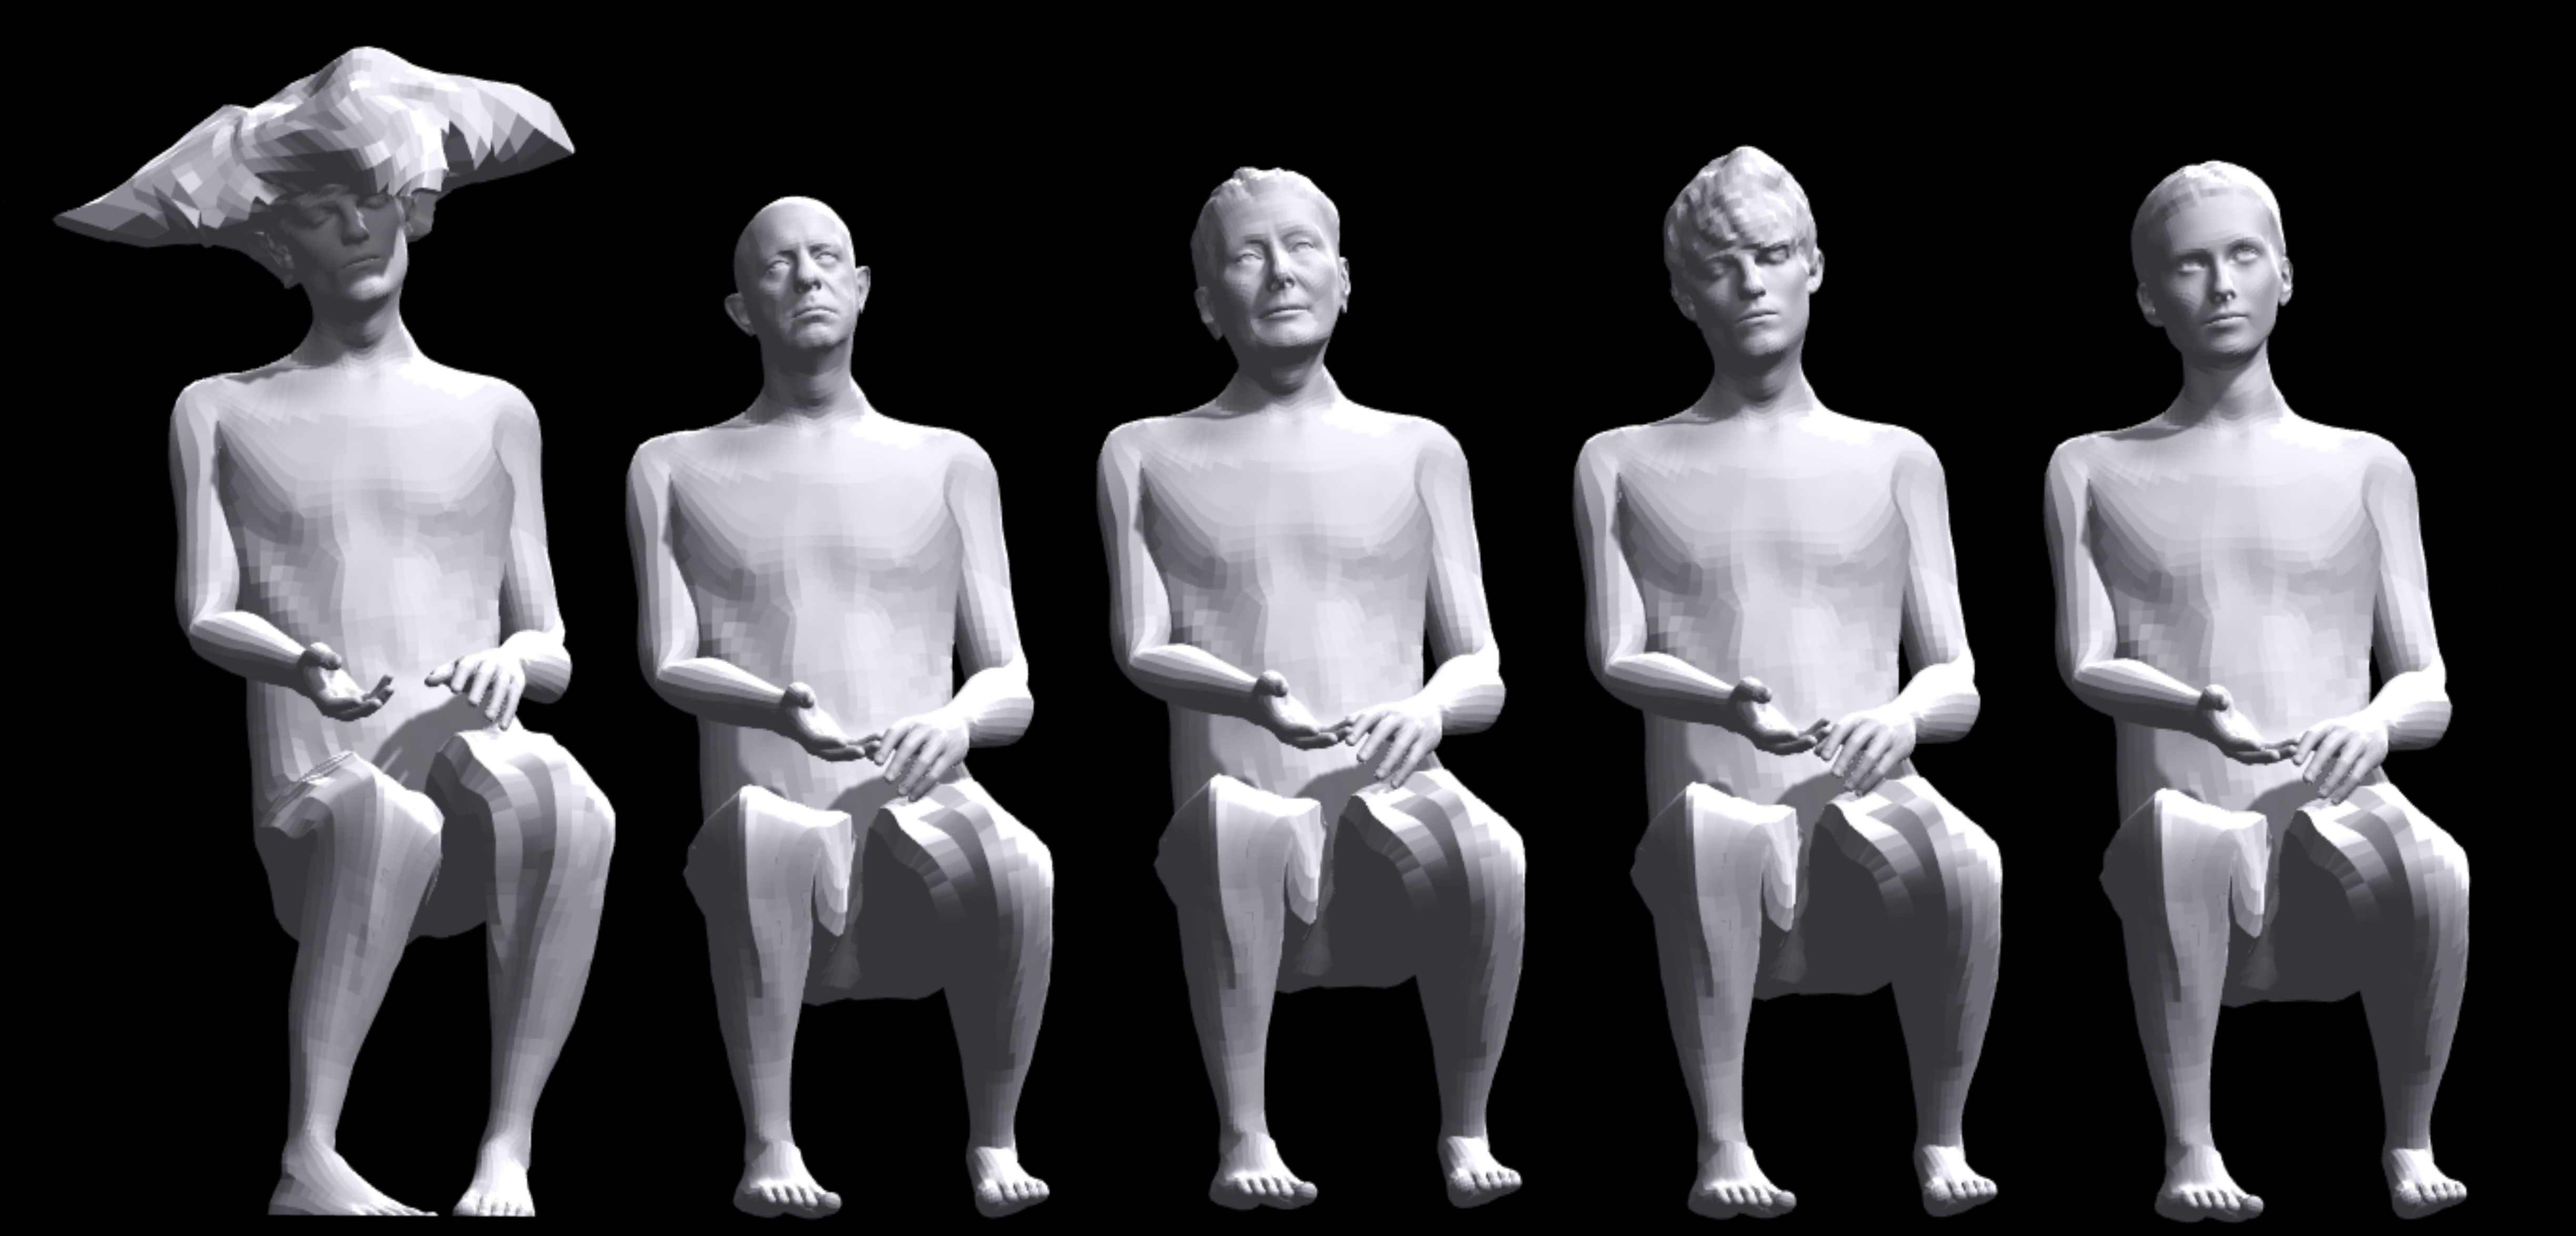
\includegraphics[width=\textwidth]{fig4}
	\caption{Various models used in the project. From left to right: Bob with hat, Old man, Vivienne, Bob, Carla.}
	\label{fig:fig4_models}
\end{figure}

\chapter{Related Work}
\label{chap:relatedwork}

Interactive agents on screens can be found in current research as an approach to entertainment, education, and training. 
While entertainment and art overlap in many areas, not many such projects have explored the more philosophical side of such an interaction as in INTRA SPACE. 
But as the main focus of this work is describing the implementation of the implemented agent system, this chapter reviews similar use-cases and installations, as well as general research regarding the topic of interactions between users and agent systems.

\section{User Interaction and Depiction of Agents}
\label{chap:userinteraction}

Fundamental research on user interactions with virtual agents in both virtual and mixed environments has been conducted in~\cite{10.1007/978-3-540-39396-2_39}, where the difference between such environments is highlighted:
\begin{quote}
	``User interaction with virtual agents generally takes place in virtual environments in which there is clear separation between the virtual actors and the user, due to the fact that in most cases, the user is in some way external to the virtual world. In Mixed-Reality Interactive Storytelling, the user’s video image is captured in real time and inserted into a virtual world populated by autonomous synthetic actors with which the user interacts. The user in turn watches the composite world projected on a large screen, following a `magic mirror' metaphor.''~\cite[p.~1]{10.1007/978-3-540-39396-2_39}
\end{quote}
The same magic mirror metaphor can be applied to the project described in this work, as \glspl{visitor}’ image data is captured and information gained from it is used to render images onto the screen. 
However, different from such mixed-reality applications, the mirror does not reflect the world of the user and instead serves as an interface to the world of the virtual agent. \\
Relevant research can also be found in the field of human-robot interaction, as robots serve as agents, controlled by \gls{ai} as well. 
While robots have a physical body and agents of this project do not, many problems apply to both alike, such as appearing human or human-like to users. 
In~\cite{stenzel2012humanoid}, it is described when and how humans view robots as robots or not, whereas~\cite{suzuki1998intelligent} describes human-robot interaction with agents using artificial emotions including learning and self-adaption features, similar to the agents in this project. 
Emotions are exhibited by visuals, lights, music, movement, behavior, etc. – methods that have been tried to represent INTRA SPACE’s agents’ emotions as well. 
In~\cite{suzuki1998intelligent}, humans interact with the robot without wearing any sensors, as the robot uses ultrasound sensor and cameras to recognize user actions. 
Furthermore, the use of the word kansei (sense, sensibility) is suggested, as it describes a field of major research in Japanese robotics – how do robots express emotions? \\
Similar research can be found in ~\cite{pereira2014improving}, which provides answers to the questions of what makes humans perceive agents as a social presence, and how can it be improved. 
They conducted a case study, in which a multiplayer board game was played together with a robot. 
The results of this study led them to establish 5 guidelines, which were a physical body, believable verbal and nonverbal behavior, an emotion system, social memory, and the simulation of social roles.
Accordingly, agents controlling robots must adhere to those rules, to be realized as a social presence by humans. 
The importance of a physical body is especially interesting in the context of this work, as the agents of this project do not possess one to the extent that is considered necessary by ~\cite{pereira2014improving}, but are merely projections on a physical screen. \\
Depiction of lifelike virtual humans is a topic of research for various applications, as is described in~\cite{mcdonnell2012render}. 
Such depictions find use in movies, games, interactive dramas, therapy, training, and marketing (see also~\cite{gratch2002creating}). 
Realistic rendering oftentimes causes a negative reaction among viewers, caused by the famous uncanny valley phenomena. 
~\cite{mcdonnell2012render} also goes into detail on motion capture and eye tracking, and presents an evaluation on the eleven different rendering styles which have been tried out over the course of their research. \\
Other topics relevant to the project and \gls{ai} development, even if not directly the focus of this work, include research on motion capture of humans, such as~\cite{moeslund2006survey}, which dictates four major steps which were used in the project of this work as well – initialization, tracking, pose estimation, and recognition. 
Tracking human gestures is a field of study that ties into various applications within modern computer science, as~\cite{wachs2011vision} argues that future human-computer interaction will enable more natural, intuitive communication resembling human-human communication by employing gesture tracking.

\section{Similar Installations}
\label{chap:similarinstallations}

FlurMax – an installation very similar to the one described in this work, containing an interactive virtual agent in a hallway to entertain \glspl{visitor}, is described in~\cite{10.1007/978-3-540-39396-2_5}. 
Another example for conversational agents can be found in web-based Eliza from~\cite{llorach2017say}. 
Such agents focus on conversation in natural human language, whereas the agents described in this work are, with a few exceptions, only able to understand and communicate via gestures. \\
More focused on the artistic side and thus more similar installations can be found in~\cite{bevacqua2014effects}, in which the effects of human-virtual agent body interaction are explored by conducting an experiment on user experience. 
The results show that the most obvious dimension to users is the so called dimension of “coupling”, which measures the level of connection between the user and the virtual agent, and is considered necessary for users to feel engaged.
\begin{quote}
	``Coupling is the continuous mutual influence between two individuals, and has a dynamic specific to the dyad. It possesses the capability to resist disturbance, and compensates by evolving the interaction. Disturbances come from both the environment and from within the individuals, depending on how they perceive the interaction.''~\cite[p.~1]{bevacqua2014effects}
\end{quote}
In the experiment, the virtual on-screen agent mirrors the user’s movements and actions, while the wizard of Oz (a person hidden from user) is able to manipulate agent actions directly, to cause disturbances within the interaction. 
The study claims that a 0.5 second delay on mirroring – meaning that 0.5 seconds would pass before the virtual agent enacts the same movement as the user did before – was found out to be the best value to cause the agent to seem less automated and more natural or intelligent. \\
A follow-up experiment is described in~\cite{bevacqua2015gestural}, which focuses once again on coupling between humans and virtual characters in an artistic context of imitation. 
It features a very similar set-up, in which the user and the agent figure mirror one another. 
The whole experience is defined as a “game”, in which the user can “fail”, by losing the virtual figures interest, caused by a lack of interaction. 
This second installation is even more similar to the one described in this work, as it features agent behavior, goals, and \gls{ai} in order to shape the interaction between the agent and the user. 
It is however notable, that the interaction with the virtual agent in INTRA SPACE was explicitly stated not to be seen as a game and thus differentiates itself from the research found in~\cite{bevacqua2015gestural}. \\
In~\cite{pugliese2011framework}, research was conducted on motion-based bodily interactions with virtual characters and methodology based on the findings is proposed. 
The experiments used a similar set-up as well, and furthermore also used pre-recorded animations in combination with real-time captured animations to bring the agents to life.

\section{Jason and Alternatives}
\label{chap:jasonandalternatives}

Jason~\cite{bordini2004jason}~\cite{Bordini:2007:PMS:1197104} is used as a platform to develop agent systems in various different contexts. 
Because of its portability by being implemented completely in Java, as well as being based on the agent programming language \gls{as}~\cite{rao1996agentspeak} which is in turn based on the \gls{bdi} model, agents in Jason can fulfill the role of an agent system for a myriad of requirements. 
The platform works as an interpreter for an extended version of \gls{as}, a \gls{bdi} agent-oriented logic programming language. 
Because it allows \glspl{mas} to be distributed over a network, its primary usage lies within distributed multi agent systems.
It offers speech-act based inter-agent communication, as well as annotations on plans. 
Users can customize features such as trust functions, selection functions, and internal actions. 
The environment, in which the agents act, can also be implemented and customized in Java. 
It is considered easy to learn and has good scalability, user friendly GUI features, good performance, and high stability. 
Finally, it is free and open source. More details on Jason, as well as an explanation why it was chosen for the project, can be found in Chapter \Autoref{chap:jason}. \\
An example for relevant agent systems implementations using Jason can be found in~\cite{ranathunga2011interfacing}, in which Jason is used for an agent platform to act within the online game Second Life and has to rely on unreliable sensor data. 
The game Second Life is generally often used as a platform for virtual agents and agent systems to act within (see also~\cite{bogdanovych2010authentic}). 
Another example is the system described in~\cite{boissier2013multi}, in which Jason is used in conjunction with Moise for agent organization and \gls{cartago} for shared environments. 
\gls{cartago}~\cite{ricci2006cartago} is a framework designed to extend \glspl{mas} with artifact based working environments. 
\gls{cartago} in combination with Jason is furthermore also used in~\cite{ricci2011environment}, which implement artifacts as abstract entities in an environment, for agents to interact with. \\
As there is already a large amount of different agent platforms available to develop agent systems with, choosing the right one for a project can be a difficult task. 
Furthermore, the wrong choice of an agent platform can lead to unnecessary work or unsatisfying results. 
In~\cite{kravari2015survey}, a vast amount of agent platform options is presented, compared, and reviewed, to help making informed decisions on which platform to use. 
Similarly, \cite{oliveira1999multi} presents an overview of what kind of research can be used for which applications in regards to \glspl{mas}. \\
An alternative to using Jason can be found in JACK~\cite{Winikoff2005}, which is considered to be the leading commercial \gls{bdi}-agent toolkit, extending Java intuitively and thus being easily portable, same as Jason. 
Another Java-based alternative would be JADE~\cite{bellifemine1999jade}, which is considered the most popular platform in the industry and academic community. 
JADE focuses on distributed applications. 
NetLogo~\cite{tisue2004netlogo} offers a multi agent modeling environment, designed after the Logo programming language, and is considered the most popular in education and research, as it is designed to be used without beforehand knowledge about programming. \\
Concurrent MetateM~\cite{Barringer1995} offers a unique language based on temporal logic for modeling reactive systems. 
It was suggested as an alternative during the development process of INTRA SPACE, and although the language itself ended up not being used, various ideas and concepts of the language were adopted and used to develop the project in the end. \\
Other approaches have agents learning from scratch to solve problems or act on their desires.
Examples include the use of back-propagation neural networks to create \glspl{ia} in intelligent virtual environments, such as in~\cite{jia2007entertainment}, in which a self-learning \gls{ai} uses such neural networks to navigate a maze-like game. \\
In~\cite{salichs2012new}, a biologically inspired decision making system is implemented, which uses emotions, such as happiness, sadness, and fear to help the \gls{ai} to learn how to act from scratch.
Similarly, in~\cite{grand1998creatures}, artificial animals using neural networks are implemented using genetics, breeding, and a biochemical system. 
They interact with humans and each other, and results show that creatures appear to learn and display emergent social behavior. 
More research on artificial life can be found in~\cite{maes1995artificial}, which ``models life as it could be, so as to understand life as we know it".

\section{Story-telling}
\label{chap:storytelling}

Software agents can be used in various ways, such as a mechanism to help computer users with work and information overload, but also purely for arts and entertainment, as interactive artificial agents are already a big part of the modern entertainment industry. 
Telling stories using agent systems is a research topic that ties closely to this work, as the virtual agents try to communicate with \gls{visitor}’s based on predefined stories. 
~\cite{brenner2010creating} presents a dynamic story based on a \gls{mas}, in which beliefs, sentiments, and goals change all the time. 
They employ plot graphs using events, temporal and causal links, beliefs, etc. to visualize stories and argue that generation of dynamic plots has not been studied sufficiently.
~\cite{10.1007/11944577_1} aims for believable agents for interactive storytelling, constructing a coherent narrative combined with user agency, by employing a drama manager (an automated story director) to orchestrate and guide agents within their system. 
A summarizing work regarding interactive narrative research can be found in~\cite{riedl2012interactive}, which describes its uses in entertainment, education, and training. 
They describe interactive narrative as a digital interactive experience with user influence, which creates a dramatic storyline. 
However, users must believe that their actions can significantly alter the direction or outcome of the story, meaning they must receive feedback to their actions and be able to comprehend the consequences, as opposed to being shown scripted stories which do not involve them. 
This problem was also encountered during this work’s project (see \Autoref{chap:sleeper}).

\chapter{The System}
\label{chap:thesystem}

As described in \Autoref{chap:about} and seen in Figure~\ref{fig:fig1_overview}, the physical set-up can be divided into multiple spaces. 
In this chapter, the spaces’ separate entities and their connections are further described and explained. 
In Figure~\ref{fig:fig5_informationflow}, the flow of data and information within the system is shown. 
The main focus lies on the agent system which is running independently inside the Render Node, containing a simulated environment and the individual agents. 
Wrappers and interfaces for communication between entities are not shown in the depiction.
\begin{figure}[h]
	\centering
	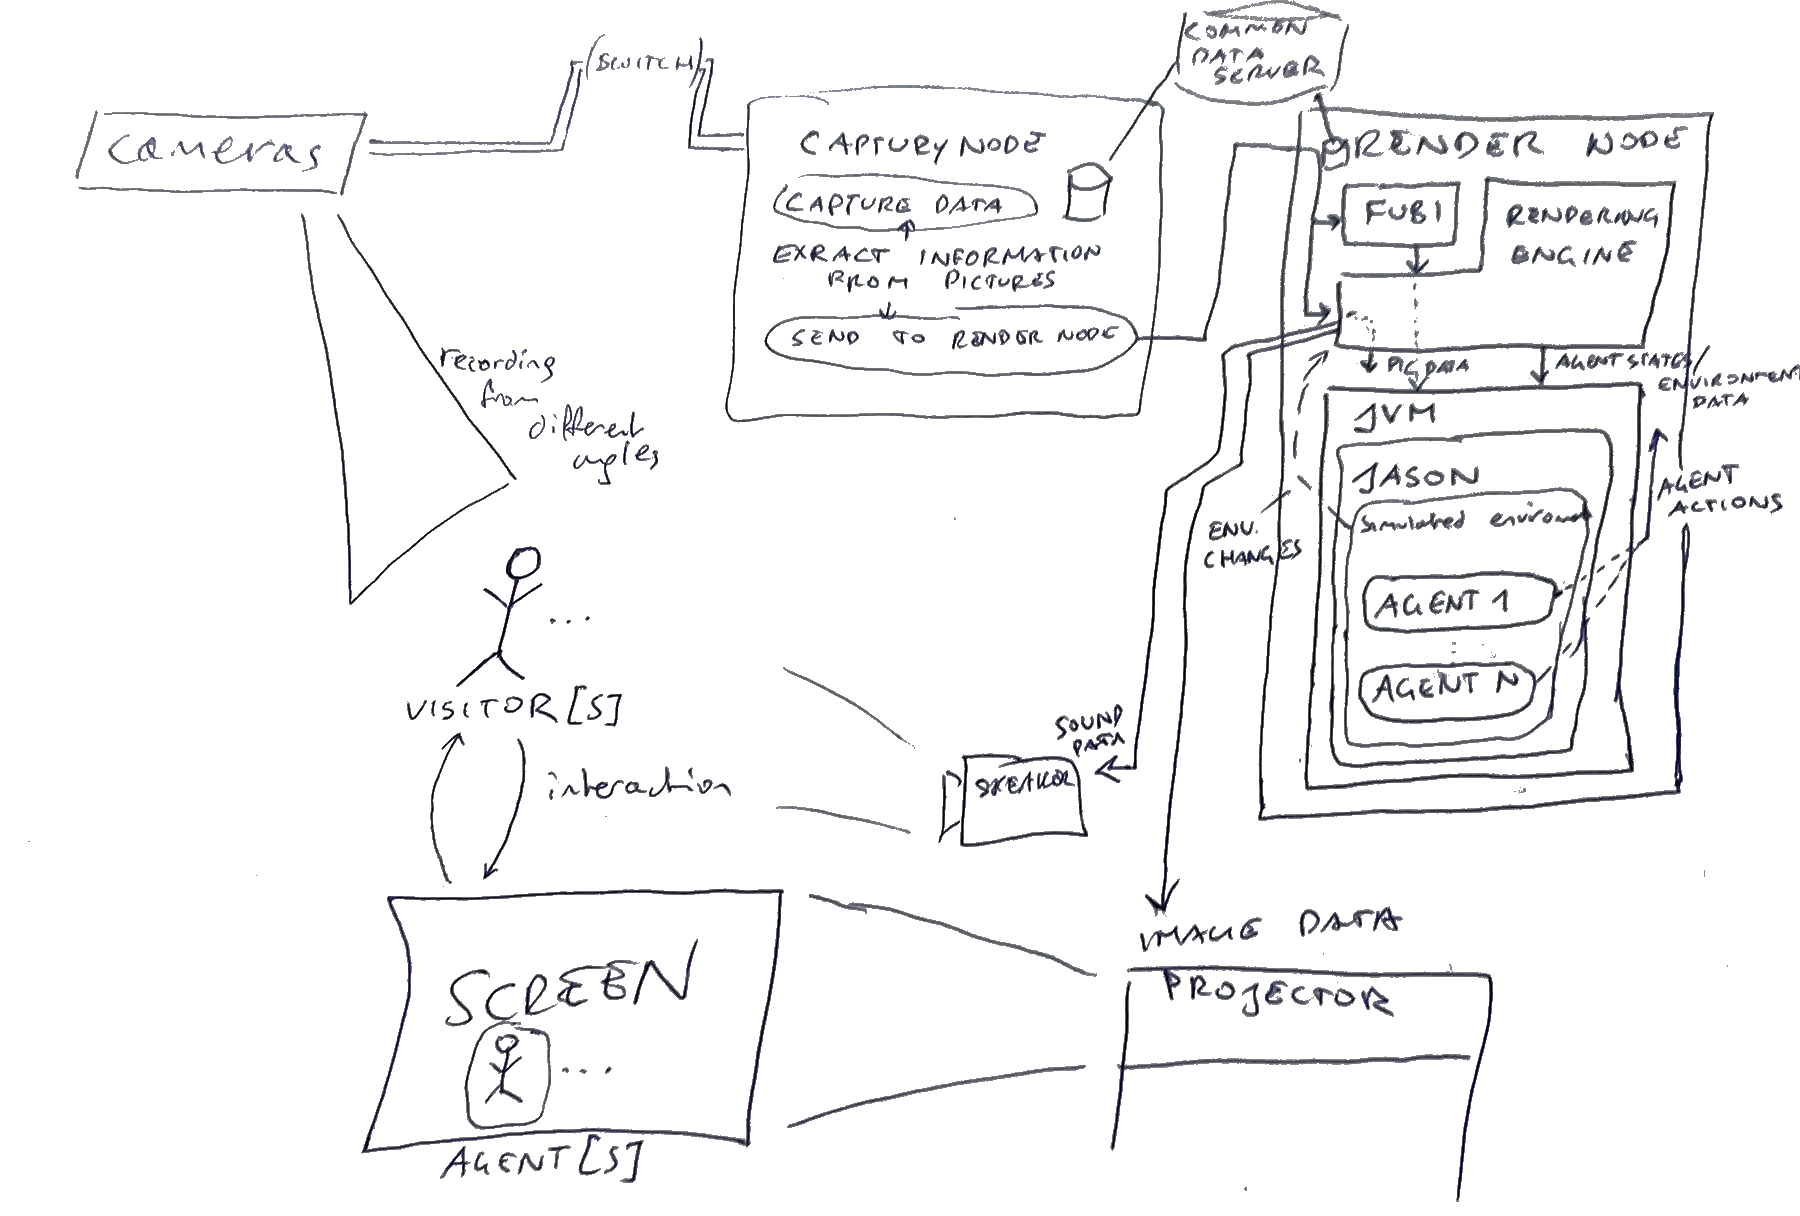
\includegraphics[width=\textwidth]{fig5}
	\caption{Simplified schematic overview of information flow within the installation.}
	\label{fig:fig5_informationflow}
\end{figure}

\section{Overview}
\label{chap:overview}

12 cameras are placed around the motion-capture space to record the \glspl{visitor}’ movements from various angles, enabling the motion-capture software The Captury Live ~\cite{capturyLive} to reconstruct a model corresponding to each \gls{visitor}. 
The model’s skeletal data can then be saved as a recording, or sent directly to the render node, which is responsible for drawing the \glspl{agent figure}. 
The render node utilizes various ways to analyze the received data – such as the \gls{fubi}~\cite{fubi}, which is able to recognize pre-defined gestures like waving or sitting. 
Data on recognized gestures is then processed by the rendering engine and shared with the running instance of the Java Virtual Machine, containing the Jason processes. 
Data communication between Java and the rendering engine was handled via \gls{udp}, by sending packets of information encoded in \gls{bson}, which is a binary data interchange format based on \gls{json}. \\
The Java thread receiving the packets processes the information and feeds it into the simulated environment, which is part of the Jason architecture. 
Agents within the environment are able to perceive it and changes within it, thus being able to react accordingly to new information. 
\Glspl{jason agent} are able to control the \glspl{agent figure} within the rendering engine by sending them commands using Jason’s custom-definable actions. 
Because of this implementation, it could be said that the actual agents within the Jason platform are not in absolute control of the on-screen \glspl{agent figure} visible to \glspl{visitor}. 
A fitting allegory might be puppet masters controlling their puppets using strings, without being able to see exactly what their puppets could see. 
As such, it is theoretically possible for the \glspl{agent figure} to fail performing commands issued to them by the \glspl{jason agent} – a problem which had to be considered during development. \\
The environment is generally considered to be an empty space, causing the simulated environment within the Jason platform to be rarely used. 
However, interactions with artifacts, such as tangible objects, sources of darkness and light, or cameras, are also possible in some agent stories. 
In such cases, the artifacts are often-times part of the simulated environment, although related calculations ultimately proved to be more efficiently done directly within the rendering engine. \\
The rendering engine is responsible for performing calculations, animation, and drawing the \glspl{agent figure} onto the screen. 
Using orthographic projection and a custom-made projection-mapping component to nullify alignment errors, the picture was drawn onto the screen using a professional projector. 
Because of physical constraints, the projectors image was reflected by two large-scale mirrors before reaching the screen (see Figure~\ref{fig:fig1_overview}). 
Finally, the large screen, suspended mid-air, functioned as a window for \glspl{visitor} to see into the world of the virtual \glspl{agent figure}. 
While \glspl{visitor} got their information about the agents from the screen, the agents got their information about the \glspl{visitor} from the cameras surrounding the \glspl{visitor}, thus completing the circle of information flow and interaction.

\section{The Room}
\label{chap:theroom}

Most of the project’s later stages were developed and executed within a single room. 
The layout of said room can be seen in Figure~\ref{fig:fig1_overview}. 
The room featured white, blank walls and a grey floor, its architecture including large pillars and arcs to support the ceiling and upper floors. 
The room’s decoration was minimalistic and simple, with notable parts being the large mirrors, some of which were used to refract the light from the projector onto the screen. 
The room’s small windows were shut during visits, as the ever-changing lighting conditions of sunlight could easily disrupt the tracking software and thus lead to unwanted movements or behavior of the agents. 
Instead, the room was illuminated by a large spot light, which was also refracted by a mirror suspended in mid-air, which directed it at the ceiling and illuminated the whole motion-capture space (see Figure~\ref{fig:fig1_overview}). \\
\Glspl{visitor} would enter the room from the other side of the room, unable to see the work spaces and motion-capture space before walking past the screen. 
The first thing they saw instead, would be the mirrors, the reflections of the \gls{agent figure} in them, and the screen from behind, which would also show the \gls{agent figure}. 
The \glspl{visitor} had to walk through the beams of light emitted from the projector and reflected by the mirrors and would often stop to observe the mirrors on the sides and on the ceiling, before entering the spaces behind the screen. \\
The motion-capture space was laid out with black flooring, for the purpose of showing \glspl{visitor} what portion of the room was focused on by the cameras, equalling the portion of the room they could freely move in while being tracked. 
Roughly in the middle of the flooring was a spot marked with a subtle X-symbol, which served the purpose of showing \glspl{visitor} where to stand during the donning phase (see \Autoref{chap:donning}), because the motion-capture software required new persons to stand within a predefined position in the room at the start, so as to accurately locate and capture them. 
Leaving the black flooring would cause some cameras to lose the \gls{visitor}’s image, thus increasing the likelihood of problems in capturing their motion data. 
During the final installation, a “bed” akin to an extremely low table covered in pelt and a larger piece of felt fabric, functioning as a potential blanket, were sometimes placed into the motion-capture space prior to the arrival of \glspl{visitor}, which can be seen in Figure~\ref{fig:fig7_mocapspace}. 
As the final installation used the sleeping agent (see \Autoref{chap:sleeper}), these objects could be used as a part of the interaction with said agent.
\begin{figure}[h]
	\centering
	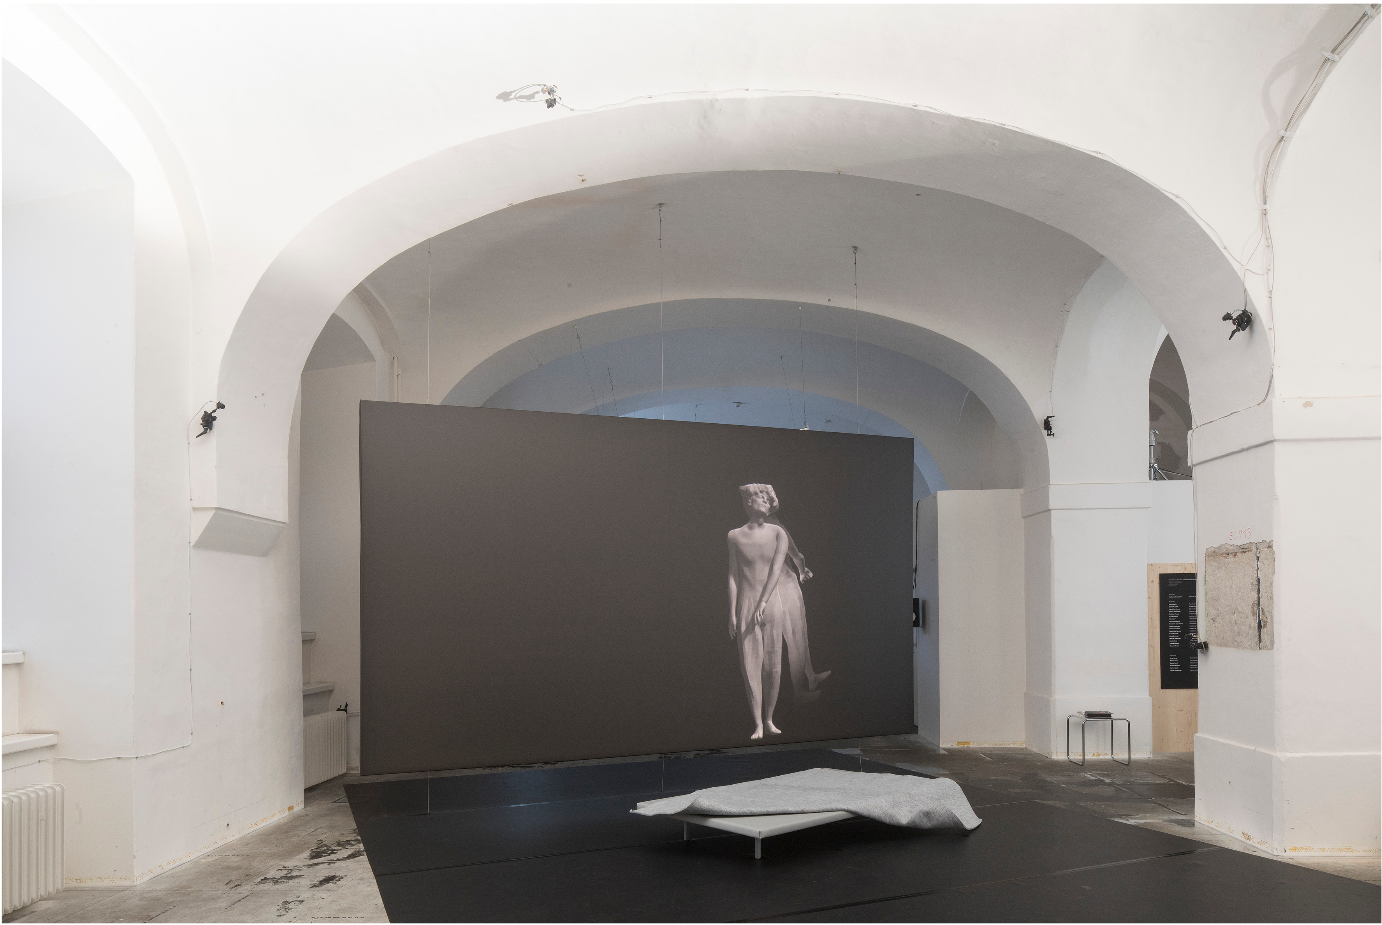
\includegraphics[width=\textwidth]{fig6}
	\caption{View onto the motion-capture space and the screen (Picture taken by Günter Richard Wett)}
	\label{fig:fig7_mocapspace}
\end{figure}

\section{Donning}
\label{chap:donning}

Regardless of which version of the project is being used, the \gls{visitor} has to go through a set of pre-defined motions first, to enable the motion-capture software to estimate body proportions. 
This process was dubbed ‘donning’, as the \gls{visitor} could see a visualized skeleton being laid over his own body, akin to clothing or armor, on the Captury Node screen (see Figure~\ref{fig:fig6_skeletons}). 
Such skeletons had the option to be saved within the software and used again at a later date. 
This functionality proved to be insufficient however, as the data used to find the corresponding person to each skeleton was based solely on color data delivered by the cameras, thus causing slight changes in color, such as different clothing or even different times of the day, to cause mismatches. 
It was thus decided, that every \gls{visitor} had to start with the donning phase before they could interact with the virtual \gls{agent figure} on the screen. 
During development, it was tried to have the agents on the screen lead \glspl{visitor} through this phase. 
This lead to multiple problems, such as \glspl{visitor} realizing the \gls{agent figure} as autonomous before emancipation has occurred. 
Furthermore, as the \glspl{agent figure}’ communicative abilities were limited to gestures, it proved hard to understand to first-time \glspl{visitor}, which in turn lead to suboptimal results during the donning phase. 
The project team realized the importance of this phase being executed as well as possible, as improper results lead to erroneous tracking and thus increased the amount of unwanted behavior by the agent. 
Thus it was decided to explain the donning phase to \glspl{visitor} using on-screen text and audio-based instructions. \\
The donning process itself consists of multiple suggested motions and postures, which are supposed to be performed and sometimes repeated by the \glspl{visitor}, to allow the motion-capture software to make accurate estimates of their body proportions. 
The first pose consists of upright standing, with both arms held about 30 centimeters in front of the chest. 
Shoulders, elbows, and hands would be roughly on the same level under optimal conditions. 
After assuming such a pose, \glspl{visitor} are asked to move their upper bodies and turn around on the spot, before having to move their lower bodies and perform stretches and similar motions. 
Results of the donning process vary greatly and are dependent on various factors, including lighting conditions, the color of worn clothing, time since the last system calibration was performed, as well as the speed in which the aforementioned motions were performed. 
Most of these factors could be contained by various methods, but unpredictable \gls{visitor} behavior always represented a risk for problems occurring in the process of donning.
\begin{figure}[h]
	\centering
	\begin{subfigure}[b]{0.5465\columnwidth}
		\centering
		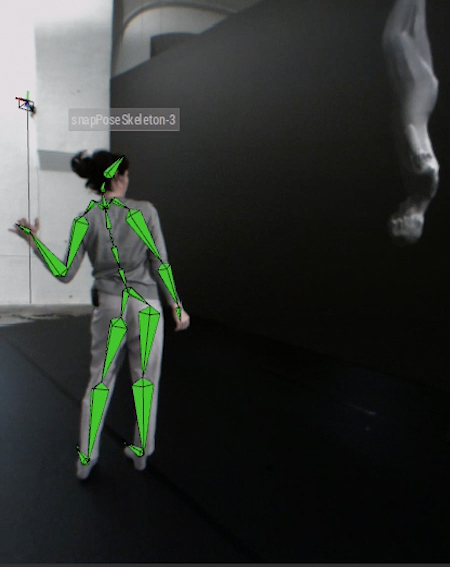
\includegraphics[width=\textwidth]{fig7-1}
	\end{subfigure}
	\begin{subfigure}[b]{0.439\columnwidth}
		\centering
		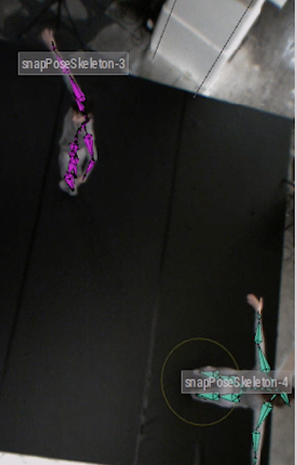
\includegraphics[width=\textwidth]{fig7-2}
	\end{subfigure}
	\caption{Some \glspl{visitor} with their assigned skeletons drawn onto them.}
	\label{fig:fig6_skeletons} 
\end{figure}

\section{Jason}
\label{chap:jason}

Jason is an open source software developed by Jomi F. Hübner and Rafael H. Bordini~\cite{bordini2004jason}~\cite{Bordini:2007:PMS:1197104}.
It offers a development platform for \glspl{mas} using an extended version of \gls{as}, which is an agent-oriented programming language designed by Anand Rao in 1996~\cite{rao1996agentspeak} and based on the \gls{bdi} model. 
This chapter offers a short introduction to the various concepts related to Jason, and shows how \gls{as} is implemented using the Jason \gls{mas}. \\
As was explained in \Autoref{chap:jasonandalternatives}, Jason is developed in Java and allows for a high degree of customization, although some critical areas are impossible to change without changes in the source code.
It offers a platform for both developing and executing agent systems, either locally or employing a network, and is further extendible by other agent-system frameworks, such as \gls{cartago}~\cite{ricci2006cartago} or JADE ~\cite{bellifemine1999jade}. \\
Jason was chosen because of low complexity and being easy to learn. 
Furthermore, it fit the project’s requirements and allowed customization in critical areas. 
It was also recommended by experts in the field of \gls{ai} development. 
As is further explained in \Autoref{problems}, in hindsight, other platforms and approaches might have worked as well, or even better, for the task that was at hand.

\subsection{Agents}
\label{chap:agents}

Agents in the context of \gls{ai}, often also referred to as \glspl{ia}, describe autonomous entities, which are able to perceive, as well as interact with their environment. 
More specifically, \glspl{ia} perceive the environment through sensors and act through actuators (see Figure~\ref{fig:fig71_agentinteraction}). 
\Glspl{ia} are rational, which means they must act in ways that maximize their performance and progression towards their goals, based on their currently held knowledge at any time~\cite{russell2016artificial}. 
Depending on the type of \gls{ia}, it might use a history of everything it perceived so far, or only beliefs it holds at the moment, to make a decision. \\
\Glspl{ia} are implemented using agent programs, which are responsible for defining which actions are to be taken after new information is perceived. 
Agent programs can be implemented by following various design patterns. 
Jason employs goal-based agents, which use pre-defined plans to reach their active goals. 
Agent programs are then embedded within a certain architecture, which supplies sensors and actuators.
Jason offers this architecture in the form of an environment, which is implemented by a customizable Java class. 
Usually, the architecture functions as the interface to the physical world, in which sensors and actuators are used. 
In the case of this project however, agents only exist and act within a virtual world, with some sensors providing data from the physical world, while others are targeted at the virtual world. 
The agents are thus not directly able to interact with the physical world, while perceiving both spaces. 
For the sake of the abstract model shown in Figure~\ref{fig:fig71_agentinteraction} however, there is no distinction necessary between the physical and the virtual space. 
Agents are thus defined as the combination of an agent program and an architecture~\cite{russell2016artificial}. 
\begin{figure}[h]
	\centering
	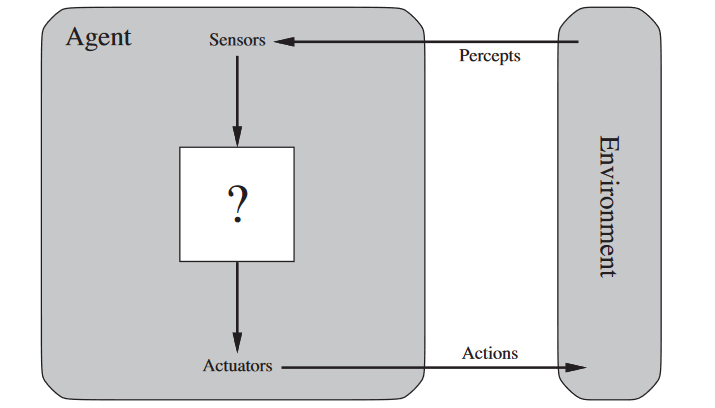
\includegraphics[width=\textwidth]{fig7-3}
	\caption{Abstract model for agent-environment interaction. (Source:~\cite[p.~35]{russell2016artificial}.)}
	\label{fig:fig71_agentinteraction}
\end{figure}

\subsection{Multi-agent Systems}
\label{chap:mas}

Agent systems, more often \glspl{mas}, are systems consisting of multiple \glspl{ia}. 
A \gls{mas} is able to host multiple \glspl{ia} acting independently of each other, which are also being able to communicate and interact with each other, as well as with the environment. 
Thus \glspl{mas} offer a distributed system for \glspl{ia} to work within, allowing for solutions to complex problems which might not be possible by using centralized approaches. 
Especially if the problem itself is distributed in nature, using a \gls{mas} can lead to efficient and easy-to-understand solutions~\cite{ferber1999multi}. 

\subsection{Belief-desire-intention Model}
\label{chap:bdi}

The \gls{bdi} model is based on a psychological model by philosopher Michael E. Bratman, who was also involved in developing the software model. 
The \gls{bdi} model separates the concepts of beliefs, desires, and intention within the \glspl{ia}, to allow them to both choose what to do, as well as follow through with their chosen plans. 
The plans to be executed by the \glspl{ia} however are usually not created by the agents themselves, but are designed and implemented by their developers~\cite{rao1996agentspeak}. \\
Beliefs describe all information an \gls{ia} has about is environment. 
They are either perceptions about the environment, introduced via sensor data, or mental notes established by the \glspl{ia} themselves – as a result of other beliefs, events, or their own actions. 
Beliefs do not have to be true and can change in the future. 
In addition, they can also possess a percentage-based truth value to represent the likeliness of being accurate. 
Adding or removing beliefs from an \gls{ia} causes respective events to trigger, which in turn may modify other beliefs or trigger plans to be executed. \\
Desires represent states that individual \glspl{ia} want to accomplish, regardless of whether they are currently acting towards fulfillment of such states or not. 
As soon as the \gls{ia} starts pursuing a desire, it has acquired a new goal. 
Contrary to desires, goals must be mutually exclusive. 
This means that \glspl{ia} may need to make decisions on which single desire to act on, if multiple possible but mutually exclusive desires are present. \\
Goals are reached by following plans, which consist of multiple actions, which in turn may be represented by other plans. 
Furthermore, a single goal could also be reachable by multiple plans, which could all be possible to follow at a single point in time. 
In such cases, the agent is expected to choose only one applicable plan. 
In the case of the Jason \gls{mas}, this can be done in two ways – either by making only one goal viable to be pursued at a time by defining mutually exclusive contexts (pre-conditions), or by using custom selection functions defined within the Java-based environment. 
If neither are implemented, the default selection function chooses the first applicable plan instead, which may not be the most cost-efficient one. 
Once the \gls{ia} has actively started executing such a plan, the desire which caused the plan to be followed is referred to as an intention. Intentions are thus defined as desires an \gls{ia} has committed to.  

\subsection{AgentSpeak}
\label{chap:as}

\gls{as}, formerly called AgentSpeak(L), is a logic-based, agent-oriented programming language, which was originally designed as an abstract language without actual implementation, for the purpose of gaining insight and understanding of the \gls{bdi} model~\cite{rao1996agentspeak}. 
The language offers a way of equipping agents with knowledge about certain pre-defined plans, also referred to as know-how, so that agents can make use of those plans to fulfill their goals or react to changes in their environment. 
\gls{as}, as well as Jason, were designed for cooperative agents, focusing on allowing \glspl{ia} to communicate and interact with each other easily. 
A brief explanation on \gls{as} syntax, as it is used in Jason, can be found in the next subsection.

\subsection{Jason Syntax}
\label{chap:syntax}

Jason offers an actual implementation of the \gls{as} language, while also adding additional functionality – for example in the form of various customizable components within the agent and environment Java classes. 
Agents within \gls{as} are defined by their initial beliefs and their plans. 
A simple example for this can be seen below.
\begin{verbatim}
    alive.
		
    +alive 
	    <-  .print(“Hello World”).
\end{verbatim}
The first line specifies an initial belief, which the \gls{ia} adds to its belief base as soon as it starts being active. 
The belief is saved as a literal, similar to traditional logic programming languages such as Prolog. 
Such literals often take the form of predicates, to express properties of certain objects. 
The literal in this example however, is a so-called atom, which displays no properties except for existing within the belief base. 
The period following the initial belief functions as a syntactic separator, similar to semicolons in Java. \\
The second line displays a very simple example of a plan. 
The first part, \verb|+alive|, defines when the plan is to be executed. 
The plus symbol represents the addition of a new belief, thus the plan will be executed whenever the belief \verb|alive| is added to the belief base. 
The arrow operator separates the plan’s head from its body, where instructions can be found. 
In this case, there is only one instruction, which is an action to be executed as soon as the plan is started. 
As can be seen in the example, the plan will print out the words \verb|Hello World| into the console, whenever it is triggered. 
If the agent were to be started now, it would first add a new belief in the form of \verb|alive| to its belief-base, which would cause an event to trigger. 
This event is represented by \verb|+alive|, which happens to have an applicable plan assigned to it, which is then executed. 
It is important to note, that the content of the belief is insignificant in this case. 
Instead of \verb|alive|, other words or expressions could be used in the same way, as long as they start with a lower-case character, which causes them to be recognized as atoms.
An example for a more complex plan can be seen below.
\begin{verbatim}
    +alive 
        <-  !eat;
            .print(“I have finished eating”).

    +!eat : not eaten(_)
        <-  eat_food;
            +eaten(1);
            !!eat.

    +!eat : eaten(X) & X < 5
        <-  eat_food;
            -+eaten(X+1);
            !!eat.

    +!eat : eaten(X) & X >= 5 .
\end{verbatim}
The first plan looks somewhat similar to the one in the first example. 
It is triggered with the addition of the belief \verb|alive| and finishes by printing out a message. 
In between, there is an additional step, which starts with an exclamation mark and ends with a semicolon.
The latter separates multiple steps of a single plan, as opposed to the period, which concludes plans or initial beliefs, whereas the exclamation mark precedes goals. 
In this case, a new goal is added, which is \verb|eat|. 
Only after the goal has been fulfilled, the plan continues being executed, and the message is being printed out on the console. 
The newly added goal \verb|eat| has three plans associated with its addition, which are marked by \verb|+!eat|. 
Furthermore, all of those plans have an additional component in their plan head, which is placed in between a colon and the aforementioned arrow operator. 
This part is called the context, which works like a pre-condition for the plan to be chosen. 
It must offer a binary result, based on which the plan either becomes viable to be chosen or not. 
The first context reads \verb|not eaten(_)|, which means the plan can be chosen as long as there is no belief called \verb|eaten| within the \gls{ia}'s belief base, with any value associated to it, as the underscore represents a wildcard. 
The second context is satisfied as long as the value held within the belief \verb|eaten| is smaller than five, whereas the third context will become satisfied as soon as the same value equals five or higher. 
This code thus represents an example of three mutually exclusive plans for the same goal, as was discussed in \Autoref{chap:bdi}.\\
The first plan for \verb|+!eat| executes the action \verb|eat_food| as its first step. 
This action has to be implemented within the Java-based environment class and return a success flag, for the plan to be able to continue. 
After the action has finished, a new belief is added in the form of \verb|+eaten(1)|, in which the plus represents the addition of the belief that follows after it. 
The belief adds the attribute of \verb|eaten| to the value of \verb|1|, which could also be an atom, such as \verb|apple| for example. 
As stated before, the addition of a belief also triggers an event, however there is no plan associated with \verb|+eaten(1)| or \verb|+eaten(_)|, thus no plan is executed. 
The last step once again causes the agent to pursue the goal of \verb|eat|. 
The double exclamation mark causes the current plan to continue without waiting for the newly added plan to finish. 
In this case, it serves only as recursion optimization, as it does not leave the finished \verb|+!eat| plans on the stack. \\
The second plan is mostly the same, with a difference in the second line. 
Expressions starting with upper-case characters in \gls{as} function as variables, in which other literals can be stored. 
In this example, \verb|X| is unified with every available value for the attribute of \verb|eaten|, causing it to take the value of \verb|1| the first time it is called. 
\verb|X| is used again in the expression \verb|-+eaten(X+1)|, which causes all beliefs of \verb|eaten| to be removed from the belief-base first, before adding a new \verb|eaten| belief with the value of \verb|X+1|. 
The third plan for \verb|+!eat| does not have a body at all, which means that the goal is fulfilled as soon as this plan is chosen. 
It thus serves as a termination condition for the recursive functionality of the \verb|!eat| goal. \\
In conclusion, the example code above would cause the agent to \verb|eat_food| five times, before stopping and printing out a message. 
For this to happen, it would need to start by adding the belief \verb|alive| to its belief-base, for example in the same way as in the first code example.

\section{Input Data}
\label{chap:inputdata}

Input data refers to all data sent from the rendering engine to the Jason \gls{mas}. 
The kinds of information that are transmitted this way can be seen in~\ref{tab:jason_input}.
\begin{table}
%	\centering
	\begin{tabular}{p{0.5\linewidth}|p{0.44\linewidth}}
		\toprule
		Information content & Reference within agent source code  \\
		\midrule
		Visitors’ gestures recognized by \gls{fubi} or by the rendering engine	& actorstate \\ %\hline
		Visitors’ position within the physical room							& actorposition; actordistancetoscreen \\ %\hline
		Visitors’ movement speed											& bodymotion \\ %\hline
		Donning status (percentage; 100\% means donning is finished)		& actorscaling \\ %\hline
		Information regarding the active camera								& camerapos; cameraborder \\ %\hline
		Positions of objects or artifacts									& objectposition \\ %\hline
		Current scenario (story)											& scenario \\ %\hline
		Agents’ current action (for example: idle, live, mid-animation)		& agentstate \\ %\hline
		Agents’ position within the virtual room							& agentposition \\ %\hline
		\bottomrule
	\end{tabular}
	\caption{Information transmitted from the rendering engine to the Jason \gls{mas}}
	\label{tab:jason_input}
\end{table}
All input data is processed by the Java thread receiving the information via \gls{udp}. 
The thread then introduces the pre-processed data into the simulated environment. 
If data of the same kind was already available, it is updated instead. 
For example, positional data of all active agents and \glspl{visitor} is updated periodically. 
In some cases, the data is instead only removed from the environment, because it is no longer up-to-date. 
Furthermore, information in the environment can be made visible to all agents or only to specifically chosen ones. 
A supervisor agent, which does not have a visual representation on the screen and only runs on the Jason platform, is responsible to orchestrate the agents respective to the currently active scenario, telling them when to start and when to stop their performances. 
As such, some of the data is only made available to the supervisor agent. \\
All data is sent from the rendering engine, where it was processed from input coming from The Captury, calculated using the physics engine or script functions, or forwarded from \gls{fubi}. 
Use of \gls{fubi} was minimized in the later stages of the project, as it oftentimes proved not reliable enough. 
Instead, custom scripts within the rendering engine were developed to detect specific gestures and send relevant information to the agent system. \\
During development, some calculations were made within the \gls{mas}, by the agents themselves, which proved to be inefficient and oftentimes produced code that was very hard to read and comprehend afterwards. 
Thus it was changed later and calculations were almost exclusively performed within the rendering engine or within the Java-based environment.  \\
During development, one of the problems that became clear was latency caused by the communication between the rendering engine and the \gls{mas} environment. 
As both were usually executed on the same machine, network latency did not pose a problem. 
However, processing of received data on the side of the \gls{mas} was handled by multiple queues, as well as Jason’s inherent reasoning cycle, which is responsible for detecting changes in the perceived environment, thus updating the currently held beliefs of all agents, and subsequently triggering all relevant events linked to any changes in beliefs. 
As it turned out, it was possible for this system to be overloaded with input data, which in turn caused it to lag behind on execution and ultimately caused it to not be able to react in time to any changes. 
It became apparent, that it was important to control the amount of information sent from the rendering engine to the \gls{mas}, so as to ensure flawless execution and timely reactions. 
Because of this, the rate at which constantly changing information was sent out from the rendering engine had to be limited to a frequency which was less than the frame rate of the rendering engine, whereas one-time changes were always sent out immediately.

\section{Output Data}
\label{chap:outputdata}

Output data refers to all data sent from the \gls{mas} to the rendering engine, which consists mostly of actions the agents wish to take, but also includes meta-information like currently active scenarios and signals regarding the state of the agent system in general, such as whether it is ready to be used. 
To send out orders to the rendering engine, \glspl{jason agent} use custom actions, which are defined within the environment class, which is written in Java. 
The environment class uses threads to communicate with the rendering engine, sending \gls{bson}-encoded packets via \gls{udp}. \\
Commands issued by the \glspl{jason agent} are either related to a pre-recorded animation, a desired state, or both. 
Examples for animations include gestures like waving or shrugging, as well as general movements like jumping or swooping. 
States are divided into the three main states, of which only one can be active at a time and which include “idle”, “\gls{live}”, and “animating”, as well as meta states, which can be active in combination with the main states.
“Idle” is the default state, in which the agent stands upright and plays a subtle animation loop to appear unengaged. 
The \gls{live} state causes the agent to mirror the \gls{visitor}’s movements. 
Switching into \gls{live} is not always easy however, for reasons which are further explained further below. 
“Animating” is a common state for all animations, which is used whenever the agent is currently in the middle of executing a pre-recorded animation. 
Meta states are oftentimes coupled with a certain animation, of which they usually come as a natural result – for example “lying down” causes agents to switch to a “sleeping” state. 
Furthermore, some states and commands are exclusive to certain scenarios, such as the bat scenario, which included states for the agent appearing upside down on the ceiling of the virtual room within the screen, as well as commands to switch from the ceiling to the floor or vice versa.\\
Because agents are not directly in control of their actions, as was described in \Autoref{chap:overview}, but rather send commands towards the \glspl{agent figure} within the rendering engine, they need to know whether the action was executed and furthermore, if the action caused any changes within the environment. 
\gls{as} and Jason generally define every agent action as a process that might be successful or unsuccessful. 
This implies that agents get feedback whether their actions succeeded or not. 
If custom actions are implemented using Java, these actions must terminate with return-values indicating success or failure, so that the agent can act accordingly. 
If a single action takes a while to complete, the agent pauses its currently followed plan and waits for a response on whether the action has succeeded or not. 
However, this proved to be problematic in the scope of this project for many reasons. 
One of which was the fact, that agent actions had to be interruptible by the \glspl{jason agent} themselves, in case the situation changed and the agent had to react. 
In some cases, single animations spanned timeframes of more than ten seconds, in which agents might have not been able to react to changes. 
Jason’s framework offers solutions to this problem as well, such as concurrent plans and reactions to new events being able to cancel and discard other currently pursued goals. 
Such an approach proved to be in need of detailed error-handling, as agents would otherwise cancel their goals too often without replacing them, causing them to lose all active behavior in many cases. 
Furthermore, it was oftentimes unforeseeable how long certain actions would take. 
For certain actions, such as synchronizing with the \gls{visitor} or interacting with an artifact within the virtual room, the virtual \gls{agent figure} would have to move to a certain position first, before being able to execute the action. 
Depending on where the \gls{agent figure} was located before the command was issued, as well as other circumstances, the time needed to complete the action could vary greatly. 
This makes it harder for the \glspl{jason agent} to plan beforehand on when to issue follow-up steps or whether or not they are in a position to react to certain events. \\
Instead, \glspl{jason agent} in this project were caused to behave differently. 
External actions, which would be sent out to the rendering engine, always return successes as soon as the packet is sent out. 
Thus, the agents command flow will not be interrupted and agents can continue on with their plans. 
However, \glspl{jason agent} are made to doubt whether their actions are actually successful or not, thus making the agents check the status of their respective visual agents, to determine if the actions have actually been performed after they have sent out the order. 
For example, whenever the agent would perform a SwitchToLive, it commands the visual agent to synchronize with the \gls{visitor} and to start copying the \gls{visitor}’s movements. 
However, it is not clear beforehand how long the virtual \gls{agent figure} will take until it starts mirroring the \gls{visitor}, as it has to move to the same position within the mirrored reality before being able to start. 
The \gls{jason agent} is nevertheless able to continue its plan after it sent out the command. 
It is capable of checking the state of the visual agent, whether it is \gls{live} or not – meaning whether it has successfully started mirroring the \gls{visitor}, and thus determine when to continue with other parts of the plan that depend on that state. 
Yet if the \gls{jason agent} wants to interrupt the process of the visual agent synchronizing with the \gls{visitor}, it can do so at any time as well, by sending out a new command. \\
This behavior could effectively also be performed by multi-threading agents, which would pause one plan while waiting for an action to finish, while concurrently following other goals, which would take over in case the action needed to be stopped. 
Such a design was also employed whenever the agent needed to react to changes in its environment, as changes were also able to cause the agent to pursue a new goal. 
For the story-based main goals of this work however, this proved complicated, as splitting them up into multiple goals was not an easy task and proved too complex within the scope of this project.\\
This decision also made it possible to perform smooth transitions from one pre-recorded animation to the next, as \glspl{jason agent} were allowed to queue up multiple animations while the visual agent was still mid-animation.
If \glspl{jason agent} had to wait for a response from the animation engine to confirm their command has been executed successfully, there would have been a brief window, after the visual agent finished the animation and before a new command was sent out by the \gls{jason agent}, in which there were no clear instructions on what the agent within the rendering engine was supposed to do. 
In this project, the visual agents defaulted to their idle state in such cases, in which they stood upright and performed a looping idle animation. 
Even if only a fraction of a second passed in between the end of one animation and starting the next one, the idle state would be clearly visible to spectators of the visual agent on the screen, often in the form of quick and erratic movement. 
To prevent this from happening, \glspl{jason agent} were given the ability to queue up commands for execution by the visual agents instead. 
This allows animations to chain into each other without triggering the default idle state, thus creating more natural looking agent movement. \\
Furthermore, communication between agents, to share beliefs, intentions, or other information is directly supported in Jason. 
Agents were thus able to warn other agents if they intended to perform certain actions, tell them what to do, or request information or cooperation. 
This was commonly used while developing multi-agent scenarios including artifacts, so as to not cause both agents to interact with the same artifact if that was not possible. 
It was also used as a shortcut to add specific new perceptions to other agents, for example if one of the visual agents waved at the other, the waving agent also directly communicated with the other agent at the same time, instead of letting the second agent perceive it via the environment. 
This is counter to the design philosophy of the agent system, but proved to be adequate.
A possible scenario, in which differences may occur, would be if the second agent was looking in the opposite direction and would not be able to see the first agent waving at them. 
However, cases like this could also be handled by polling information about positions and directions of the \glspl{agent figure} directly by the agents themselves.

\chapter{Implementation}
\label{chap:implementation}

This chapter goes into detail about the process of developing and implementing the agent system using Jason. 
First, an initial approach is described and explained, which was developed and tested right after work on the agent system has started. 
Some specific agent stories are highlighted, as well as their results explained. 
Afterwards, the final approach, which was implemented after multiple discussions within the project team and consulting with experts, is introduced and explained. 
Finally, this chapter also offers insight into how communication worked within the core team of the project, using visualizations to plot and discuss various agent stories. 
In this context, stories refer to textual or visual representations of what is expected of an agent, whereas scenarios refer to the implementations of said stories in the form of \glspl{jason agent} within the \gls{mas}.

\section{Initial Approach}
\label{chap:initialapproach}

During the initial approach, various stories that had been written and designed previously by the project team were to be implemented into a \gls{mas} using Jason. 
As described in \Autoref{chap:about}, at the start of development, the rendering engine was able to draw an \gls{agent figure} onto the screen, which would proceed to mirror any movements of \glspl{visitor} tracked by the motion-capture system. 
The \gls{jason agent} was then supposed to infuse the visual agent with a will of its own, so that it could emancipate itself away from being a mere reflection of the \gls{visitor}. 
The agents’ behavior, movements, animations, goals, and reactions all differed depending on the active scenario. \\
Two of the first stories developed by the project team were the octopus agent and the bat agent. 
The way in which those stories were brought to paper can be seen in Figure~\ref{fig:fig8_octopus}. 
As can be seen in the intention part of the figure story, additional features like a visible environment within the virtual space, as well as the use of sound to enhance the experience were originally planned, but not implemented completely within the final product. 
Before those first two stories were implemented however, it was decided to develop a simpler story for purposes of setting up the environment properly and getting a general look at how agent development in Jason worked within the scope of the project. 
This simple story became known as the waving agents, featuring two active agents with the goal of causing at least one of the \glspl{visitor} to wave their hand towards the screen. \\
Throughout development of the waving agents, it became clear that their behavior could be divided into somewhat independent phases. 
Phase zero usually consists of the donning phase (as described in \Autoref{chap:donning}), in which the \glspl{visitor}’ body proportions are estimated by the motion-capture system, to allow the software to track visitors’ movements throughout the designated motion-capture space. 
After donning is completed, the so called \gls{live} part follows, in which the \gls{agent figure} would synchronize with the \gls{visitor}’s position on the other side of the screen and start mirroring the \gls{visitor}’s movements.
\begin{figure}[h]
	\centering
	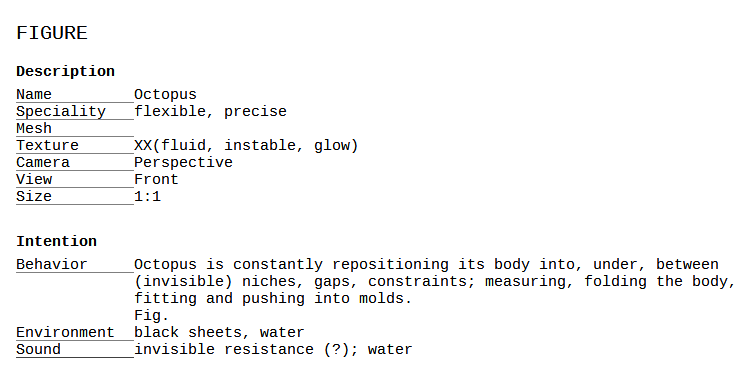
\includegraphics[width=\textwidth]{fig8}
	\caption{Octopus agent story, written by Christina Jauernik.}
	\label{fig:fig8_octopus}
\end{figure}
\begin{figure}[h]
	\centering
	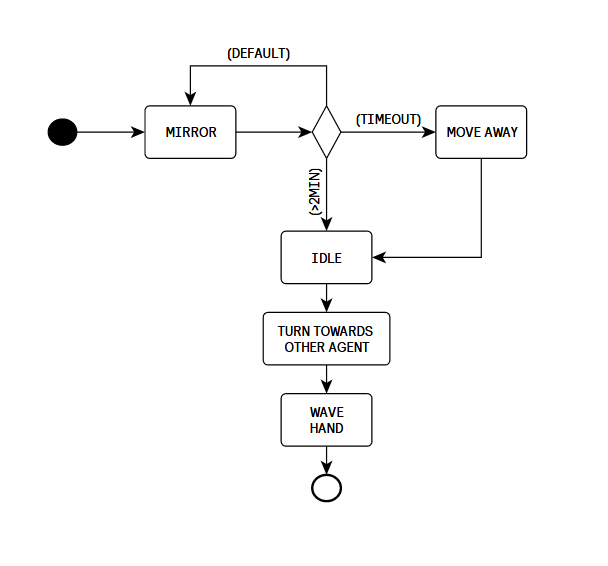
\includegraphics[width=\textwidth]{fig9}
	\caption{Waving agent model, phase 1, digitalized by Simon Oberhammer.}
	\label{fig:fig9_wave}
\end{figure}

\subsection{Waving Agents}
\label{chap:waving}

As was mentioned above, the waving agent scenario features two agents and requires two \glspl{visitor}. 
Each \gls{visitor} is assigned their \gls{agent figure}, which becomes apparent to the \glspl{visitor}, as soon as the respective agents figures start mirroring their movements. 
The end-goal of the scenario consists of getting at least one of the \glspl{visitor} to wave at the screen, towards the \glspl{agent figure}. 
The origin of the scenario lies within already implemented functionality of the \gls{fubi} framework, which made it possible to recognize waving as a gesture performed by motion-captured individuals. 
Furthermore it was argued that \glspl{ia} necessarily needed an ultimate goal, so as to be able to act within the Jason \gls{mas} – which is why the goal of getting the \glspl{visitor} to wave was defined as such. \\
In the first phase, after the \gls{live} part, emancipation occurred and the waving agents start pursuing their scenario-specific goals. 
During this stage of development, the trigger for agents to stop being \gls{live} and start moving on their own is purely based on time. 
At first it was decided to have this behavior start exactly two minutes after donning was completed, although this time span was later reduced to a random amount in between 50 and 70 seconds. 
As soon as both agents are finished with \gls{live}, the first \gls{agent figure} turns towards the second \gls{agent figure} and waves at them. 
If there is not enough space in between the two agents to make the animated gesture certain to be visible, the first agent decides to move away from the other agent on its own, so as to create enough space. 
After the first \gls{agent figure} has successfully executed the waving animation, phase one ends and phase two starts. 
A simple model depicting phase one, using notation similar to that of UML activity diagrams, was created by the project members and can be seen in Figure~\ref{fig:fig9_wave}. 
The visualization only depicts the process of the first agent’s activities and simplifies the way the agent checked for distance between the two \glspl{agent figure}. \\
Within phase two, the two \glspl{agent figure} continue by waving their hands at each other, before turning towards the camera and waving towards the \glspl{visitor} as well. 
In case at least one of the \glspl{visitor} waves back, the figures express joy by clapping their hands, before switching back to \gls{live}, mirroring the \glspl{visitor}’ actions indefinitely. 
If the \glspl{visitor} do not wave back, the two agents try three more times by waving towards the camera, before giving up and fading away from sight. 
The scenario was later extended by an additional goal of getting both \glspl{visitor} to wave back towards the \glspl{agent figure}. \\
The scenario generally worked well after several iterations. 
However, problems with the \gls{fubi} framework arose early, causing it to be unable to recognize waving \glspl{visitor} consistently. 
Furthermore, the binary result of either celebration or failure made the scenario very similar to a game in nature. 
This went against the idea of the installation, as the idea was to distance the experience from games and to promote more natural interaction between \glspl{visitor} and the \glspl{agent figure}. 
Development on the waving agents was thus stopped, and development on the previously mentioned animal-based agents begun.

\subsection{Octopus Agent}
\label{chap:octopus}

The octopus agent story was one of the first ones to be implemented as an agent scenario. 
The general concept can be understood from Figure~\ref{fig:fig8_octopus}, which offers descriptions of both the octopus \gls{agent figure}, as well as a its behavior and environment. 
The agent itself can be considered more of an experimental agent, based on the idea of the magic mirror, which was embodied by the screen. 
The octopus agent is supposed to interact with its respective \gls{visitor}’s body reflection, for example by squeezing the \gls{agent figure}’s body into the empty space between the \gls{visitor}’s arms and chest, or similar openings.
Different from a magic mirror installation however, the \gls{visitor}’s body was not visible on the screen, but only the \gls{agent figure}. \\
The idea of the octopus agent was ultimately not pursued or developed very far, as it proved too complicated to record fitting animations and use them appropriately. 
Additionally, the concept itself was very confusing to \glspl{visitor}. 
Combined with suboptimal \gls{agent figure} movements and decisions, \glspl{visitor} did not properly understand the mode of interaction. 
Thus the whole scenario was deemed unsuitable for the given project scope.

\subsection{Bat Agent}
\label{chap:bat}

The bat agent story focused on an agent with bat-like, animalistic behavior. 
The core concept of the bat is the ability of the \gls{agent figure} to switch between standing on the floor and upside down on the ceiling. 
For example, the bat agent would start off by sleeping upside down on the top of the screen, before waking up and eventually moving down to the floor to find itself on the same level as the \gls{visitor}. \\
The agent scenario is focused on various kinds of interactions and different outcomes depending on the \glspl{visitor}’ behavior. 
It was the most extensively developed agent scenario up to this point, with a large number of iterations, as well as many concepts which were tried out before being removed from the agent scenario again. 
Different from the waving agents, it is designed for one \gls{visitor} at a time, although multiple bat agents could be employed for multiple \glspl{visitor}. 
In the case of multiple bat agents being active at the same time however, they will not interact with each other – the only inter-agent communication that occurs is to prevent the agents from overlapping and occupying the same spot of the screen. \\
Another noteworthy feature of the bat agent story is that agents are able to show more open hostility in interactions with \glspl{visitor}, for example by attacking or swooping towards them. 
Such animations are hard to interpret by \glspl{visitor} however, as the missing dimension of the orthogonal projection, in addition to the impossibility of physical interaction between \glspl{agent figure} and \glspl{visitor} made it hard to tell what the agents are aiming at. \\
Bat agents were the first agent scenario to use emotional scales, such as for example the level of timidity ranging from zero to one hundred. 
The value of those scale variables would change depending on actions of the \gls{visitor}, and would influence how the bat \gls{agent figure} would react to certain events. 
The waving agents had a similar concept, in which their emotions would simply change from one state to the other – such as either being happy, sad, or neutral. 
In later agent scenarios, such numerical values are further used to impact other dimensions of the interaction, such as the speed of the \gls{agent figure}’s animations or the angle in which it would face the \gls{visitor}. \\
Furthermore, bat agents have the ability to deploy additional \glspl{agent figure} and give them commands. 
These \glspl{agent figure} have various roles, such as instructing the \gls{visitor} during the donning phase, while the bat agent figure was sleeping upside down on the ceiling, or appearing next to the sleeping bat in a similar manner, such as to appear like a group of sleeping bats. \\
The bat agent scenario was in development significantly longer than previous agent scenarios. 
However, it was ultimately stopped and abandoned in favor of a different scenario, because the bat \gls{agent figure}’s behavior was deemed too hard to understand and the upside-down, pre-recorded animations did not turn out the way the project team envisioned them. 
Additionally, the bat agent’s behavior was deemed too reliant on reactions to \gls{visitor} actions. 
The goal was instead to develop an agent that interacted with the \gls{visitor}, but would also provoke interaction in case the \gls{visitor} did not act first. 
This meant that the agent story had to encompass both reactive parts to \gls{visitor} input, as well as pro-active parts for the agent to pursue their own goals. 
The agent story introduced in the next chapter focuses more on autonomy and pro-active behavior of the \gls{agent figure}. \\
A small part of the bat agent program’s source code can be seen below. 
It shows the reaction of the bat agent to a certain \gls{visitor} action under certain circumstances. 
Most of the bat agent program consisted of similar reactions to \gls{visitor} input.
\begin{verbatim}
// visitors putting their hands together while agent figure 
// remains on the ground causes bat-like agent figure to go 
// back to the ceiling
    +actorstate(ACTOR, STATE) : my_actor(ACTOR) & not animating 
    & phase(3) & STATE == handstogether & onGround
        <-  +animating;	           // currently mid-animation
            -onGround;             // not on ground level
            switchToIdle;          // stop moving, go idle
            !waitForIdle(250,0);   
            switchToCeiling;       // agent figure to ceiling
            !waitForIdle(2000,0);	
            switchToLive;          // mirror visitor movements
            -animating.            // no longer mid-animation
\end{verbatim}

\subsection{Sleeper Agent}
\label{chap:sleeper}

The sleeper agent scenario went through the highest amount of iterations and was eventually used in the final installation of the project. 
The agent story’s main idea was based on a figure that gets exhausted through movement and wants to go to sleep, to recover, before being able to interact with the \gls{visitor} again. 
Similar to the bat agent story, it was designed for one \gls{visitor} at a time, while utilizing multiple instances of the same agent in the case of multiple concurrent \glspl{visitor}. 
As can be seen in Figure~\ref{fig:fig10_sleeperState}, the actual agent story and the implementation both took the form of a finite-state machine after several iterations of development. \\
After three minutes of mirroring the \gls{visitor} in the \gls{live} state, the \gls{agent figure} will emancipate and distance itself, seek the invisible virtual bed within the virtual space, and lie down to sleep. 
If the \gls{visitor} joins the \gls{agent figure} in lying down – either on the ground or on the provided bed (as explained in \Autoref{chap:theroom}), the agent would warm up to the visitor, by increasing an internal value called sympathy. 
This value would increase whenever the \gls{agent figure} was asleep and the \gls{visitor} was either detected as lying down, based on specific bones of the body being within a certain vertical range of each other, or as long as the \gls{visitor} was close enough to the screen. 
In the same way, if the \gls{visitor} moved away too far from the screen and was not lying down, it would cause the sympathy value to decrease. \\
The goal or milestone of the scenario during the iteration displayed in Figure~\ref{fig:fig10_sleeperState}, is to arrive at the dream sequence after the \gls{visitor} lies down with the \gls{agent figure} for long enough to reach the upper limit of the sympathy value. 
This sequence would play pre-recorded audio and offer an ending to the experience, after which interaction with the agent is no longer possible. 
This was the first time a state with no way to interact and no way to change it was introduced, as it was originally planned to continue the story after this point-of-no-return with a second milestone in mind, similar to the waving agents which change their goal from having at least one \gls{visitor} waving towards the screen to having both \glspl{visitor} waving their hands at the same time. 
This second milestone was however never implemented before the whole scenario for the sleeper agent was reworked. \\
Other noteworthy states are also part of the scenario, which implemented various experimental features, such as changing cameras or environments. 
During the deep-sleep state, which occurs after the sympathy value is raised high enough, the camera changes to a perspective camera, placed inside of the \gls{agent figure}’s head – thus granting the \gls{visitor} sight of what the \gls{agent figure} would see. 
Because the virtual space the \gls{agent figure} resides in is completely empty most of the time, the first thing to appear on the screen in this state is usually nothing but black background. 
As the agent is \gls{live} during this phase, mirroring its respective \gls{visitor}’s movements, it is possible for the \gls{visitor} to see the \gls{agent figure}'s hands or whole body from the perspective of the \gls{agent figure}, if they move accordingly. 
Furthermore, if more than one \gls{visitor} is present and has an agent assigned, it was also possible to see the other \gls{agent figure} in this state. 
Differently placed cameras were also experimented with, such as one placed within the \gls{agent figure}’s hand, or one placed within its knee. 
Further experimental features include visible environments within the virtual space, such as one filled with mirrors in which the \glspl{agent figure}’ reflections can be seen, although the mirrors cannot directly be interacted with. \\
The scenario furthermore includes varying animations for the same activities, such as lying down, sleeping, and getting up again.
Various parameters, such as animation speed or rotation around the agent’s own axis are also changed depending on the situation or the current sympathy value. 
As mentioned before when explaining the dream sequence, this scenario also incorporates sound, for the most part in the form of spoken language, but also in the form of unintelligible whispering for atmospheric purposes. \\
Because the story of the sleeper agent was mapped out as a finite-state machine (see Figure~\ref{fig:fig10_sleeperState}), the implementation follows this model as well. 
Each state of the state machine is implemented as a separate plan, which is triggered whenever the goal of pursuing the respective state as a goal is added. 
These goals are added via various means, such as finishing a single state’s plan, as a reaction to \gls{visitor} behavior, or by reaching certain sympathy values. 
This can also be seen in the agent program code shown below. 
\begin{verbatim}
    +sympathy(S) : max_negative_sympathy(MNS) & S <= MNS
        <-  !!switchToPhase(11);    
        .drop_desire(adjust_sympathy).

    +!phase(11) : true
        <-  environment(narcotic);
            setTimedZoom(0,1);
            setXRotation(0, 10);
            playanimation(narcotic_sleep_loop, 1, 1, 1);
            ?my_actor(ACTOR);
            ?actorposition(ACTOR,X,Y,Z);
            -+narcotic_position(X, Y, Z).
\end{verbatim}
Commands starting with question marks symbolize test goals, which attempt to retrieve information from the belief base. 
In this case they are used to initialize variables which are later on stored as a separate belief. \\
It is important to note, that this implementation and usage of Jason – in the form of a state machine – is not the way the Jason platform was intended to be used. 
It does not follow the principles of agent programming, such as utilizing delegated goals or agents balancing being goal-driven and reactive. 
Delegation of goals implies telling an \gls{ia} what to achieve, but not how to achieve it, so that the \gls{ia} can pick the appropriate plan to achieve its goal by itself. 
Because this implementation offered almost no alternative plans for the various states, there was no flexibility available to the \gls{ia}. 
Furthermore, the various state-machine-based goals are oftentimes not true goals in the sense they are supposed to be in the context of an agent platform, as they do not describe a concrete state of affairs to be brought about. 
On the other hand, it could be argued that reaching a certain state within the state machine is also a state of affairs, although a more abstract one. 
Further guidelines and concepts of Jason and \gls{as} which are not represented well in this scenario include responsiveness, as agents would oftentimes completely ignore \gls{visitor} actions of all kind during certain states, as well as inter-agent communication and cooperation, which is after all one of the major features and selling points of the Jason \gls{mas}. \\
The results of this implementation are accordingly unsatisfactory. 
As a polar opposite to the bat agent’s behavior, which consists of almost only reactive parts, this incarnation of the sleeping agent almost never directly reacts to the \gls{visitor}’s actions. 
Interaction is always very one-sided, with the agent performing in front of the \gls{visitor}, occasionally verifying the \gls{visitor}’s position and gestures. 
Starting with the donning phase, the \gls{visitor} is instructed by the \gls{agent figure}, before the agent goes \gls{live} and allows the \gls{visitor} to experience the \gls{agent figure} mirroring their movements. 
Afterwards, the \gls{jason agent} starts telling its story and interaction is further reduced, as the agent is animated most of the time and the \gls{visitor}’s role is reduced to that of a spectator, with very limited and unclear options for interaction. \\
The story itself can unfold in a couple of ways, akin to branching paths that all lead to the same end, which is represented by the dream sequence. 
However, because there is no real interaction between the \gls{visitor} and the \gls{agent figure}, it was considered by many \glspl{visitor} to be more similar to watching a movie or a lecture, than to interpersonal interaction. 
Repeated \glspl{visitor} also noticed how the story will always lead to the same end with not too much variance, as some of the optional states are quite hidden, because of specific pre-conditions which are unclear to onlookers – such as standing up again at specific point in time after lying down. 
Project members also expressed their wishes for more variance, less predictability, more possible interactions, and most importantly, indeterministic behavior instead of deterministic one.
This meant, that randomness should play a larger role within the agent scenario, and that the agent should not always choose the same way to act or react under certain conditions. \\
After consulting with experts on how to continue, it was decided to scrap the current agent program and develop a new one from scratch. 
Because the general concept of the sleeper agent was kept, animation files and features within the rendering engine could continue to be used, thus reducing the amount of effort the fresh start entailed. 
However, as the agent program should no longer be based on a finite-state machine, development as well as graph-based visualization of the agent stories had to change drastically.
\begin{figure}[h]
	\centering
	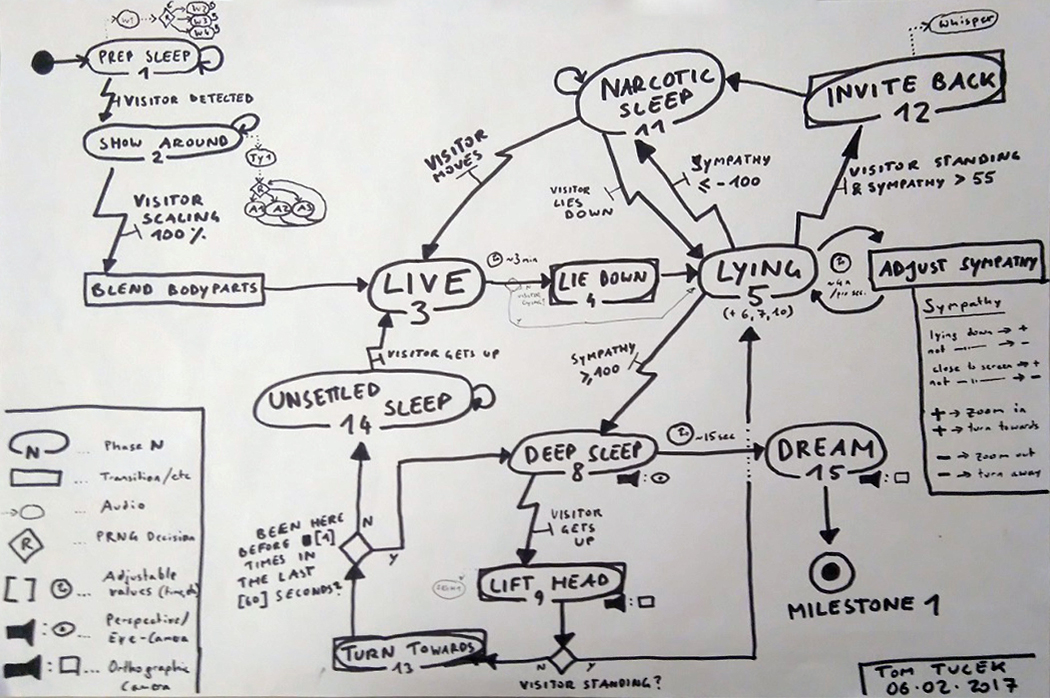
\includegraphics[width=\textwidth]{fig10}
	\caption{Sleeping agent state machine, hand-drawn during discussion.}
	\label{fig:fig10_sleeperState}
\end{figure}

\section{Final Approach}
\label{chap:finalapproach}

During the consulting phase with experts from the field of agent development, it was suggested to take a look at other agent development platforms, which might be better suited to the requirements of the project.
Explicitly, Concurrent MetateM~\cite{Barringer1995} was recommended, which is a multi-agent language similar to Jason, but uses temporal logic to generate agent behavior. 
It would allow agents to act in less obviously formulaic ways, as plans would be automatically and incrementally constructed based on temporal logic rules within the agent program. 
This would allow agents more flexibility for varying actions under the same circumstances as well. \\
However, because of the late stage during the project it was decided to not switch to MetateM, as embedding it into the current environment, learning the appropriate usage of the language and the different way of thinking in regards to temporal logic would take too long for the project to be finished in time. 
Instead, a new way of implementing agents in Jason was inspired by MetateM, which was referred to as the \gls{island system} within the project team. 
It was based on an approach to cause more indeterministic and emergent behavior amongst agents, as was requested before. 
Agents are supposed to decide on their next actions on their own, instead of only reacting to the \gls{visitor}, but actions of the \gls{visitor} would also influence which actions agents could take next, in addition to direct reactions to certain \gls{visitor} behavior. \\
The general concept is based on a graph similar to a state machine, but with no direct transitions leading from one state to another. 
The graph also displays states in the form or ovals, which are considered the name-giving islands within a vast ocean of white background to be navigated by the agent. 
Islands have pre-conditions attached to them, which must be fulfilled in order for the island to be accessible. 
If the agent wants to get to a certain island, it might have to cross other islands first, so as to fulfill the goal island’s pre-conditions. 
Furthermore, if the agent has no specific goal, it considers all islands accessible to it at the time and decides indeterministically – at random – where to go. 
This approach is closer than the state-machine-based approach to the way Jason is intended to be used, but some elements, such as the random selection amongst available islands, can be considered violations of Jason’s principles. \\
Various conditions were defined using logical rules in Jason itself, which allows use of rules in the same style as the Prolog programming language. 
Such rules, examples of which can be seen in the code below, are used as preconditions for the islands and were named based on the way the pre-conditions were visualized, as can be seen in Figure~\ref{fig:fig11_matr}.
\small\begin{verbatim}
    // position - left side
    b1 :- my_actor(ACTOR) & actorposition(ACTOR, X, Y, Z) & X < -0.5.
    // right side
    b2 :- my_actor(ACTOR) & actorposition(ACTOR, X, Y, Z) & X > 0.5.
\end{verbatim}
\normalsize The agent story was once again called “sleeping agent”, with its general behavior once again based on an agent that had to go to sleep after becoming tired. 
The \gls{agent figure} generally mirrors the \gls{visitor}’s movements and accumulates fatigue based on the intensity of the movement. 
Fatigue is represented by an energy value within the agent program code and is decreasing if the \gls{agent figure} is in motion, while increasing if the \gls{agent figure} is resting. 
If the \gls{visitor}’s movement got too insignificant, the \gls{agent figure} starts moving on its own, performing actions like strolling around the room or sitting down on an invisible chair within the virtual room. 
Such actions would cause the agent to lose energy as well. 
If the \gls{visitor}’s movement gets more intense again, the agent returns back to the \gls{live} state.
Compared to the game-like installation described in~\cite{bevacqua2015gestural}, in which users had to mirror the virtual agent’s movements and vice versa, otherwise the agent would lose interest and the game was considered lost, in this project’s installation the agent mirrors the \gls{visitor}’s movements and loses interest if the movement is considered insufficient in terms of activity level, which is calculated using the distance travelled by the \gls{visitor}’s individual limbs over time. \\
If the agent’s energy gets too low for it to continue moving, it will seek rest by going to sleep. 
While sleeping, the \gls{visitor}’s interactions are once again limited. 
However, the \gls{agent figure}’s sleep phase did not last as long as in the previous installments of this agent story. 
While the \gls{agent figure} is lying asleep in its virtual, invisible bed, the \gls{visitor} has the option to wait and observe, or to lie down as well, either on the floor or on their own bed, once again provided within the physical room as explained in \Autoref{chap:theroom}. 
Because the agent will go to sleep multiple times during a single \gls{visitor}’s experience, the \gls{visitor} has multiple chances to realize this opportunity. 
If they lie down, the agent will switch to \gls{live}, mirroring the \gls{visitor}'s movements while lying down, as well as change the camera, also similar to the previous installation, to a perspective camera located within the agents hand. 
If the \gls{visitor} decides to get up again, the camera returns to normal again. 
Furthermore, if the \gls{visitor} lies down first, the \gls{agent figure} would follow suit, allowing it to recover energy even if it was not tired yet.\\
The island-based agent follows three different kinds of goals. 
The first one is a constant goal – it causes the agent to always seek movement. 
If the agent is mirroring the \gls{visitor}, and they move their bodies enough by themselves, the goal is satisfied and the agent does not have to move away from the \gls{live} state. 
The second kind of goal is triggered by \gls{visitor} actions, such as intense movement after the \gls{agent figure} stopped mirroring the \gls{visitor} causing the agent to re-synchronize with the \gls{visitor}. 
The last kind of goal is triggered by agent-internal conditions, such as the wish to rest as soon energy has reached a certain threshold. \\
Implementation of the \gls{island system} was achieved using Jason’s annotation system, to give various plans differing chances of being executed, if multiple ones were possible to be selected.
Annotations were read by the custom selector function in Java, which utilized random values to pick out of the list of weighted available options. 
The code below shows an example for two plans with the same goal and the same context, but with different bodies and annotations, which contain the chance of them being picked by the selector function. 
Accordingly, the first plan has a chance of 30, which is six times the chance of the second plan being chosen.
\begin{verbatim}
    @idling[chance(30)]	
    +!moveAround : movement(M) & M <= 0.5
        <-  .wait(200);	
            !moveAround.

    @move[chance(5)]
    +!moveAround : movement(M) & M <= 0.5
        <-  .random(R);	
            ?bound_left(BL);
            ?bound_right(BR);
            moveTo(BL + (BR-BL)*R, 0);
            !waitForIdle(1000,250);	
            !moveAround.
\end{verbatim}
Below, a code snippet for the customized selector function can be seen. It was implemented within a class called RandomOption, which extends the Jason standard Agent class and had to be referenced within the \gls{jason agent} code of the supervisor agent whenever a new agent using this selector function was to be created. 
An example for this kind of agent creation can be seen further below.
\begin{lstlisting}
/**
* Custom selector function chooses one of the options available at random.
* Reads annotations for weighted randomness, increases chance of being drawn by same factor.
*/
public class RandomOption extends Agent {
	public Option selectOption(List<Option> options) {
		List<Option> chanced = new ArrayList<>(options);
		for(Option o : options) {
			int chance = 1;
			try {
				Literal l = o.getPlan().getLabel().getAnnot("chance");
				chance = Integer.parseInt(l.getTerm(0).toString());
			}
			catch(Exception e) {}
			for(int i = 0; i < chance; i++)
			chanced.add(o);
		}
		double r = Math.random() * chanced.size();
		return chanced.get((int)r);
	}
}
\end{lstlisting}
Below, the example for creating an agent within Jason, using the \verb|RandomOption| class explained above.
\begin{verbatim}
    .create_agent(sleeper_agent1, "170329_sleeper6.asl",
     [agentClass("RandomOption")]);
\end{verbatim}
It is important to note again, that while this approach to agent development is arguably closer to the original way Jason was intended to be used, it still does not completely align with the principles of Jason and agent-oriented programming. 
Compared to the previous state-machine-based approach, this way includes both the pro-active pursue of goals, as well as reactiveness to a changing environment, especially in the form of \gls{visitor} behavior.
However, inter-agent communication and cooperation once again fell short, as the developed scenario focused more on the interaction between one agent and one \gls{visitor}, instead of incorporating multiple agents. \\
The result of this installment is an agent with very unpredictable and oftentimes hard-to-understand behavior. 
\Glspl{visitor} are oftentimes baffled and confused by what the agents are doing at any given time – as are the members of the project team. 
Although the agent program does not offer an excessively wide amount of options, the agents display a considerable amount of emergent behavior, which was not premeditated by the developer beforehand. 
Some ideas for improvements include toning down certain screen effects, like zooming, as well as decreasing the frequency of random actions undertaken by the \gls{agent figure}. 
Additionally, if more options were provided for the agent to choose from what to do at any given time, the scope of emergent behavior could be further broadened. \\
This incarnation of the sleeping agent scenario contains several other, somewhat hidden, features, such as for example a credit roll being displayed on the screen, if a \gls{visitor} stands still and displays no intense movements for at least three minutes. 
Because \glspl{visitor} generally seem to enjoy the \gls{live} part of the interaction with the \gls{agent figure} the most, a way for \glspl{visitor} to stop agents from acting on their own and go back to \gls{live}, mirroring the \gls{visitor}, was introduced. 
As mentioned before, whenever the \gls{visitor} shows a high enough activity level, the agent would return to them. 
The simple agent code for this reaction can be seen below.
\begin{verbatim}
    @react_fast_go_live
    +activity_level(AL) & AL > 2 & auto & not sleeping
        <-  -auto;
            switchToLive.
\end{verbatim}
Some \glspl{visitor} realized this very quickly and started calling the \gls{agent figure} back by waving their arms around energetically, whenever the \gls{agent figure} started autonomous actions. 
Arguably, this can be considered a very unique kind of interaction between the human and the non-human in form of the \gls{agent figure}, which was to be explored according to the original project statement. 
\begin{figure}[h]
	\centering
	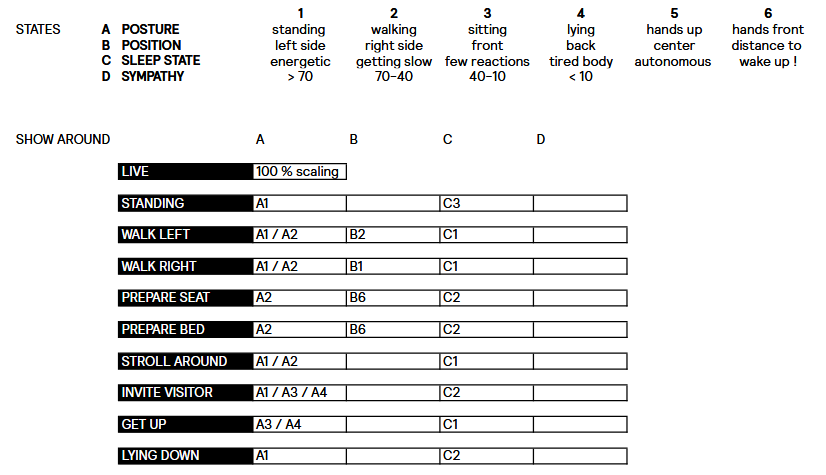
\includegraphics[width=\textwidth]{fig11}
	\caption{Sleeping agent island diagram, by Simon Oberhammer.}
	\label{fig:fig11_matr}
\end{figure}

\section{Visualization and Modelling}
\label{visualization}

One of the major problems the project team was facing during development of the agent system was communicating and visualizing agent behavior in a way for every project team member to understand and agree on. 
The project owner had specific visions of how agents were supposed to act and the development team had to understand and implement those visions. 
As such, communication of these ideas and visions was of vital importance to the project’s success. \\
At the start, agent stories and descriptions were written down as text, as can be seen in Figure~\ref{fig:fig8_octopus}. 
Such descriptions included some concrete technical data which could be directly used to adjust parameters within the rendering engine. 
However, the written descriptions of agent behavior were sometimes rather ambiguous and thus hard to understand or translate into agent program code. 
What was described was the way the agent’s behavior should appear to the \gls{visitor}, but not what caused it to act in the way it should. 
In hindsight, it would have been possible to develop agents from this starting point as well, but it would leave room for a lot of interpretation and creativity by the developers. \\
Instead, it was decided to hold small project-staff meetings to discuss and agree on possible agent behavior together. 
Drawing on paper to visualize thoughts and processes to other project members proved to be very successful, as it served both as a means of supporting verbal communication, as well as a form of documentation, which could be used for the process of implementation afterwards. 
A makeshift modeling concept based on the activity diagram of UML was employed, as it was able to tell the general gist of the story within a single look, while also encompassing all the fine det ls if necessary. 
Such drawn maps would sometimes be digitalized as seen in Figure~\ref{fig:fig9_wave}. \\
These makeshift visualizations of agent behavior were much easier to convert into agent program code, as they provided insight into possible ways how the interaction between the \glspl{visitor} and the virtual \glspl{agent figure} was envisioned to be like. 
Similar to user stories in traditional development, the diagram allowed development to focus on a certain chain of events, but at the same time made it clear, if alternative paths were supposed to exist. \\
As development went on and various agent stories were discarded in favor of new ones, the diagrams got more complex as well – an example can be seen in Figure~\ref{fig:fig10_sleeperState}. 
At the same time, the visualized agent behavior became less abstract and more akin to a finite-state machine. 
As was described in \Autoref{chap:sleeper}, converting the state machine into agent program code was rather straightforward, as every state would be implemented as a single plan attached to the goal of finishing that state. 
As the resulting code was no longer following some of the principles of agent programming, Jason’s intended usage and best practice, it was decided to start the development of the agent again from scratch. 
The new iteration was supposed to move away from the finite-state machine and instead employ a model closer to the original vision of an agent system, while also enabling the desired indeterministic behavior of agents. \\
After the paradigm shift towards the \gls{island system}, agent behavior was at first visualized in a similar fashion to the state machines again. 
The new diagrams showed unconnected states on a blank background, similar to isolated islands floating in an ocean – hence the name of the system. 
As the agent story developed, such a visualization got confusing to read very quickly, as the addition of pre-conditions, in some cases even post-conditions, made it hard to comprehend the intended agent behavior as a whole. 
The graphs were thus exchanged for separate matrices for both pre-conditions and agent behavior within certain contexts, a digitalized form of which can be seen in Figure~\ref{fig:fig11_matr}. 
This way of presenting agent stories was also possible to convert into agent program code without too much effort. 
By using logical rules based on the aforementioned matrices as pre-conditions within plan contexts (context referring to the condition for a plan being eligible at a certain point in time, as explained in \Autoref{chap:syntax}), readability was improved and plan heads could be adopted directly from the matrix-based description of agent behavior. \\
To summarize – it was a challenge to find a fitting solution to the communication problem that worked well for all parties involved. 
Text-based descriptions of agent stories were preferred by non-developers, but proved hard to implement. 
On the other hand, representations closer to actual agent program logic were hard to comprehend but easy to convert into code. 
As was mentioned at the start of the chapter, it might have been possible to work with text descriptions as well, especially if they were to focus on the experience from the standpoint of a \gls{visitor}, akin to user stories.
Multiple stories, representing various possible interactions with the \gls{agent figure}, might have helped to develop the agent system in a more traditional way. 
Furthermore, it is important to note that the chosen way of visualization has an actual impact on the development and way of thinking of agent behavior, as can be seen in the example of agent program code devolving into a finite-state machine over the course of this project.

\chapter{Discussion and Conclusion}
\label{disc}

This chapter offers a short summary, discussion and reflection in regards to the development of an interactive agent system in the context of the INTRA SPACE project, as well as some concluding remarks. 
However first off, methods of testing and evaluating the agent system, as well as problems and solutions in general are presented and discussed. 
In this context, \emph{testing} judges whether or not the agents perform what is expected of them, whereas \emph{evaluation} focuses on the quality achieved in regards to the original research project goal – the exploration of interaction between humans and virtual agents.  

\section{Testing and Evaluation}
\label{testing}

In general, both testing and evaluating the developed agent system were rather limited in scope and could not be performed in a way necessary for a project of this kind. 
One of the main reasons for this was the fact that the complete installation needed to be running for practical testing to be conducted, which was not always the case. 
As this made active testing and debugging difficult – especially at the early stages of development – a simple, custom-made Java application was used to simulate \gls{udp} responses from the rendering engine, to enable quickly available ways of both testing and debugging the Jason agent programs, as well as the Jason environment and network communication Java classes. 
In the later stages of the project, the installation was in use more frequently and the number of \glspl{visitor} increased, thus enabling pragmatic testing of the agent system more regularly. \\
Another problem was the lack of error messages within the Jason platform. 
Whenever agents stopped working, either by crashing, by not responding anymore, or by displaying erroneous behavior, the underlying reason was not easy to find or comprehend. 
This problem was solved for the most part by utilizing extensive logging via the Jason agent platform, which showed all agent logs in real-time within a separate window. \\
Evaluation of the system was also problematic, as the subjects testing the system and experiencing the interaction with the \gls{agent figure} were project team members for the most part. 
Being aware of both agent behavior and goals made it possible to test for errors, but made it more difficult to evaluate the form of interaction between the \glspl{visitor} and the virtual \glspl{agent figure}. 
Proper evaluation was thus limited to cases in which outside \glspl{visitor} interacted with the agent system. 
Because of the finite number of \glspl{visitor} and the ambiguity of feedback, the task of evaluating the system regularly turned out to be quite challenging. \\
Results of the system’s evaluation at the end of the project, based upon the feedback and comments of \glspl{visitor}, imply a high variance in the way the installation was experienced. 
Many \glspl{visitor} claimed to have realized the \gls{agent figure} as a social presence and were able to have meaningful interactions, whereas other \glspl{visitor} saw the interaction rather as a form of entertainment, akin to a game or narrative experience. 
Consequently, it could be said that the project goal of exploring, formulating, and deconstructing the ways of interaction between humans and non-humans in the form of virtual agents were met, albeit in ways which were probably not originally envisioned.

\section{Problems, Challenges, and Solutions}
\label{problems}

To summarize, the general challenges discussed in this work revolve around the following points:
\begin{itemize}
	\item Developing and embedding an agent system within a dynamic environment
	\item Finding an agent story and behavior that works well for the given goal of exploring interaction 
	\item Proper Implementation of \glspl{ia}, following the principles of general agent programming, \gls{bdi}, \gls{as}, and Jason 
	\item Communication within the project team
\end{itemize}
The first point, equaling the research question of this work, is answered by the processes described over the course of \Autoref{chap:implementation}. 
Development consisted of an iterative process, which was seemingly reset whenever an agent story was scrapped in favor of a new one. 
However, experience from previous installments would carry over, thus enabling the creation of more sophisticated agent scenarios with every iteration. 
The iterative process and regular discussions within the project team, as well as the inclusion of experts in relevant fields during such meetings, enabled a fruitful way of developing the required functionality within a dynamic requirement. 
It is important to mention that other agent system languages and frameworks might have suited the task better, if the final requirements were apparent at the start. 
However, such a massive change later on in the project was no longer possible due to resource constraints.\\
In regards to fitting agent stories and behavior, a fair number of points can be made, as to what constitutes as enabling the desired forms of interaction between agents and \glspl{visitor}. 
First and foremost, during the final stages of the project it became apparent that the instantaneous feedback during the \gls{live} phase seemed to engage \glspl{visitor} the most, as it was clear what was happening as long as the agent mirrored their movements. 
Whenever the agent took control over the figure, feedback was often too slow to be understood as such. 
It was thus considered to be important to incorporate quick reactions to \gls{visitor} interaction within the agent stories. 
If the agent only acts in a predetermined way and does not really interact with \gls{visitor}, its behavior becomes very obvious and predictable to repeated \glspl{visitor} and onlookers, thus minimizing interest, engagement, and interaction. 
To remedy this problem, indeterminism and the almost always existing possibility of instant interaction were introduced into the agents’ behavior. \\
The problem of proper implementation ties into the other problems discussed in this work, as following the principles and guidelines of the \gls{bdi} architecture, \gls{as}, and Jason more properly would have certainly produced different results than the ones achieved over the course of this project.
On the other hand, the purposeful breaking of some rules enabled the implementation of the \gls{island system}, as described in \Autoref{chap:finalapproach}. 
However, other core concepts, such as inter-agent cooperation, were still not followed appropriately and might have enhanced the interaction between \glspl{visitor} and virtual \glspl{agent figure} even further. 
The way custom action feedback was handled, as described in \Autoref{chap:outputdata}, can also be seen as a violation of Jason’s best practice, and finding a way to properly receive feedback while still being able to produce the necessary results would have helped in producing more reliable agent programs. 
Different approaches, using either different agent platforms or other implementations of \gls{ai}, such as neural networks or extensive scripts, might have also been worth pursuing and would have offered differing solutions to the ones described in this work. \\
The last of the points listed above – communication within the project team – played a significant role and had an impact, either directly or indirectly, on all areas of development. 
It was important to communicate both the imagined functionality and behavior of the agents, but also what was possible within the scope of the project in regards to cost requirements of various implementations.
In order to maximize mutual understanding of what was expected and what was possible, graphs and visualization were utilized – both analog and digital. 
Communication of agent stories, plans, and behavior worked well using graphs, especially when communicating face to face while creating them. 
The resulting diagrams furthermore enabled a faster development and testing process. 
However, they also impacted the way agent behavior was thought about and implemented, as can be seen by the negative example of finite-state-machine-based agents described in \Autoref{chap:sleeper}. \\
Further problems and challenges which appeared during the course of this project, which are not directly related to the process of agent development, include the donning stage explained in \Autoref{chap:donning}, which went through several iterations and experiments together with the agent system, before arriving at the solution of both audio-based and visual instructions at the same time. 
Although the installation was planned to be a completely autonomous one at the start, this goal was never reached, as it was considered crucial to explain the donning process to new \glspl{visitor} in addition to constant maintenance of the installation. 
Difficulties in regards to motion capture and gesture recognition also impacted agent development, as they limited the scope of gestures and interaction the agents were able to perceive. 
A solution to parts of this problem was to move away from using the \gls{fubi} framework and implement custom scripts from scratch with similar functionality within the rendering engine.

\section{Conclusion}
\label{conclusion}

In conclusion, it can be said that the developed agent system did not reach the level which was expected of it during the initial vision of the project in many aspects. 
However, it provided the required functionality of agents to be communicated with and was successfully embedded into the already existing installation. 
Some \glspl{visitor} of the installation expressed surprise, intrigue, confusion, and many other unique experiences after interacting with the agents. 
Some were fascinated by the agents mirroring their actions, others wanted to touch and interact with the agents more deeply, while some even enjoyed watching the agents act on their own. 
Many \glspl{visitor} were furthermore also eager to suggest various applicable fields, in which a similar installation, requiring no special equipment on behalf of the \gls{visitor}, could be used, such as entertainment, education, or therapy. 


% Remove following line for the final thesis.
%%% intro.tex
%% Copyright (C) 2014-2017 by Thomas Auzinger <thomas@auzinger.name>
%
% This work may be distributed and/or modified under the
% conditions of the LaTeX Project Public License, either version 1.3
% of this license or (at your option) any later version.
% The latest version of this license is in
%   http://www.latex-project.org/lppl.txt
% and version 1.3 or later is part of all distributions of LaTeX
% version 2005/12/01 or later.
%
% This work has the LPPL maintenance status `maintained'.
%
% The Current Maintainer of this work is Thomas Auzinger.
%
% This work consists of the files vutinfth.dtx and vutinfth.ins
% and the derived file vutinfth.cls.
% This work also consists of the file intro.tex.


\newacronym{ctan}{CTAN}{Comprehensive TeX Archive Network}
\newacronym{faq}{FAQ}{Frequently Asked Questions}
\newacronym{pdf}{PDF}{Portable Document Format}
\newacronym{svn}{SVN}{Subversion}
\newacronym{wysiwyg}{WYSIWYG}{What You See Is What You Get}

\newglossaryentry{texteditor}
{
  name={editor},
  description={A text editor is a type of program used for editing plain text files.}
}

\chapter{Introduction to \LaTeX}

Since \LaTeX\ is widely used in academia and industry, there exists a plethora of freely accessible introductions to the language.
Reading through the guide at \url{https://en.wikibooks.org/wiki/LaTeX} serves as a comprehensive overview for most of the functionality and is highly recommended before starting with a thesis in \LaTeX.

\section{Installation}

A full \LaTeX\ distribution\index{distribution} consists of not only of the binaries that convert the source files to the typeset documents, but also of a wide range of packages and their documentation.
Depending on the operating system, different implementations are available as shown in Table~\ref{tab:distrib}.
\textbf{Due to the large amount of packages that are in everyday use and due to their high interdependence, it is paramount to keep the installed distribution\index{distribution} up to date.}
Otherwise, obscure errors and tedious debugging ensue.

\begin{table}
  \centering
  \begin{tabular}{cccc}
    \toprule
    Distribution & Unix         & Windows      & MacOS        \\
    \midrule
    TeX Live     & \textbf{yes} & yes          & (yes)        \\
    MacTeX       & no           & no           & \textbf{yes} \\
    MikTeX       & no           & \textbf{yes} & no           \\
    \bottomrule
  \end{tabular}
  \caption{\TeX/\LaTeX\ distributions for different operating systems. Recomended choice in \textbf{bold}.}
  \label{tab:distrib} % \label has to be placed AFTER \caption to produce correct cross-references.
\end{table}

\section{Editors}

A multitude of \TeX\ \glspl{texteditor} are available differing in their editing models, their supported operating systems and their feature sets.
A comprehensive overview of \glspl{texteditor} can be found at the Wikipedia page  \url{https://en.wikipedia.org/wiki/Comparison_of_TeX_editors}.
TeXstudio (\url{http://texstudio.sourceforge.net/}) is recommended.
Most editors support the scrolling the typeset preview document to a location in the source document by \verb|Ctrl| clicking the location in the source document.

\section{Compilation}

Modern editors usually provide the compilation programs to generate \gls{pdf} documents and for most \LaTeX\ source files, this is sufficient.
More advanced \LaTeX\ functionality, such as glossaries and bibliographies, needs additional compilation steps, however.
It is also possible that errors in the compilation process invalidate intermediate files and force subsequent compilation runs to fail.
It is advisable to delete intermediate files (\verb|.aux|, \verb|.bbl|, etc.), if errors occur and persist.
All files that are not generated by the user are automatically regenerated.
To compile the current document, the steps as shown in Table~\ref{tab:compile} have to be taken.


\begin{table}
  \centering
  \begin{tabular}{rl}
    \toprule
    & Description \\
    \midrule
    1 & Scan for refs, toc/lof/lot/loa items and cites \\
    2 & Build the bibliography     \\
    3 & Link refs and build the toc/lof/lot/loa \\
    4 & Link the bibliography \\
    5 & Build the glossary \\
    6 & Build the acronyms \\
    7 & Build the index \\
    8 & Link the glossary, acronyms, and the index \\
    9 & Link the bookmarks \\
    \midrule
    & Command \\
    \midrule
    1 & \verb|pdflatex.exe  example| \\
    2 & \verb|bibtex.exe    example| \\
    3 & \verb|pdflatex.exe  example| \\
    4 & \verb|pdflatex.exe  example| \\
    5 & \verb|makeindex.exe -t example.glg -s example.ist| \\
      & \verb|              -o example.gls example.glo| \\
    6 & \verb|makeindex.exe -t example.alg -s example.ist| \\
      & \verb|              -o example.acr example.acn| \\
    7 & \verb|makeindex.exe -t example.ilg -o example.ind example.idx| \\
    8 & \verb|pdflatex.exe  example| \\
    9 & \verb|pdflatex.exe  example| \\
    \bottomrule
  \end{tabular}
  \caption{Compilation steps for this document. The following abbreviations were used: table of contents (toc), list of figures (lof), list of tables (lot), list of algorithms (loa).}
  \label{tab:compile} % \label has to be placed AFTER \caption to produce correct cross-references.
\end{table}


\section{Basic Functionality}

In this section, various examples are given of the fundamental building blocks used in a thesis.
Many \LaTeX\ commands have a rich set of options that can be supplied as optional arguments.
The documentation of each command should be consulted to get an impression of the full spectrum of its functionality.

\subsection{Floats}

Two main categories of page elements can be differentiated in the usual \LaTeX\ workflow: \textit{(i)} the main stream of text and \textit{(ii)} floating containers that are positioned at convenient positions throughout the document.
In most cases, tables, plots, and images are put into such containers since they are usually positioned at the top or bottom of pages.
These are realized by the two environments \verb|figure| and \verb|table|, which also provide functionality for cross-referencing (see Table~\ref{tab:intro} and Figure~\ref{fig:intro}) and the generation of corresponding entries in the list of figures and the list of tables.
Note that these environments solely act as containers and can be assigned arbitrary content.

\subsection{Tables}

A table in \LaTeX\ is created by using a \verb|tabular| environment or any of its extensions, e.g., \verb|tabularx|.
The commands \verb|\multirow| and \verb|\multicolumn| allow table elements to span multiple rows and columns.

\begin{table}[h] % placement specifier
  \centering
  \begin{tabular}{lll}
    \toprule
    \multicolumn{2}{c}{Position} \\
    \cmidrule{1-2} % partial horizontal rule
    Group & Abbrev & Name \\
    \midrule
    Goalkeeper & GK & Paul Robinson \\
    \midrule
    \multirow{4}{*}{Defenders} & LB & Lucus Radebe \\
                               & DC & Michael Duburry \\
                               & DC & Dominic Matteo \\
                               & RB & Didier Domi \\
    \midrule
    \multirow{3}{*}{Midfielders} & MC & David Batty \\
                                 & MC & Eirik Bakke \\
                                 & MC & Jody Morris \\
    \midrule
    Forward & FW & Jamie McMaster \\
    \midrule
    \multirow{2}{*}{Strikers} & ST & Alan Smith \\
                              & ST & Mark Viduka \\
    \bottomrule
  \end{tabular}
  \caption{Adapted example from the \LaTeX guide at \url{https://en.wikibooks.org/wiki/LaTeX/Tables}. This example uses rules specific to the \texttt{booktabs} package and employs the multi-row functionality of the \texttt{multirow} package.}
  \label{tab:intro} % \label has to be placed AFTER \caption to produce correct cross-references.
\end{table}

\subsection{Images}

An image is added to a document via the \verb|\includegraphics| command as shown in Figure~\ref{fig:intro}.
The \verb|\subcaption| command can be used to reference subfigures, such as Figure~\ref{fig:intro:full width} and~\ref{fig:intro:half width}.

\begin{figure}[h]
  \centering
  \begin{subfigure}[b]{0.45\columnwidth}
    \centering
    
\includegraphics[width=\textwidth]{TU_INF_Logo_gray}
    \subcaption{The header logo at text width.}
    \label{fig:intro:full width}
  \end{subfigure}
  \begin{subfigure}[b]{0.45\columnwidth}
    \centering
    
\includegraphics[width=0.5\textwidth]{TU_INF_Logo_gray}
    \subcaption{The header logo at half the text width.}
    \label{fig:intro:half width}
  \end{subfigure}
  \caption{The header logo at different sizes.}
  \label{fig:intro} % \label has to be placed AFTER \caption (or \subcaption) to produce correct cross-references.
\end{figure}

\subsection{Mathematical Expressions}

One of the original motivation to create the \TeX\ system was the need for mathematical typesetting.
To this day, \LaTeX\ is the preferred system to write math-heavy documents and a wide variety of functions aids the author in this task.
A mathematical expression can be inserted inline as $\sum_{n=1}^{\infty} \frac{1}{n^2} = \frac{\pi^2}{6}$ outside of the text stream as \[ \sum_{n=1}^{\infty} \frac{1}{n^2} = \frac{\pi^2}{6} \] or as numbered equation with
\begin{equation}
\sum_{n=1}^{\infty} \frac{1}{n^2} = \frac{\pi^2}{6}.
\end{equation}

\subsection{Pseudo Code}

The presentation of algorithms can be achieved with various packages; the most popular are \verb|algorithmic|, \verb|algorithm2e|, \verb|algorithmicx|, or \verb|algpseudocode|.
An overview is given at \url{https://tex.stackexchange.com/questions/229355}.
An example of the use of the \verb|alogrithm2e| package is given with Algorithm~\ref{alg:gauss-seidel}.

\begin{algorithm}
  \SetKw{BreakFor}{break for}
  \KwIn{A scalar~$\epsilon$, a matrix $\mathbf{A} = (a_{ij})$, a vector $\vec{b}$, and an initial vector $\vec{x}^{(0)}$}
  \KwOut{$\vec{x}^{(n)}$ with $\mathbf{A} \vec{x}^{(n)} \approx \vec{b}$}
  \For{$k\leftarrow 1$ \KwTo maximum iterations}
  {
     \For{$i\leftarrow 1$ \KwTo $n$}
     {
        $x_i^{(k)} = \frac{1}{a_{ii}} \left(b_i-\sum_{j<i} a_{ij} x_j^{(k)} - \sum_{j>i} a_{ij} x_j^{(k-1)} \right)$\;
     }
     \If{$\lvert\vec{x}^{(k)}-\vec{x}^{(k-1)}\rvert < \epsilon$}
     {\BreakFor\;}
  }
  \Return{$\vec{x}^{(k)}$\;}
  \caption{Gauss-Seidel}
  \label{alg:gauss-seidel} % \label has to be placed AFTER \caption to produce correct cross-references.
\end{algorithm}

\section{Bibliography}

The referencing of prior work is a fundamental requirement of academic writing and well supported by \LaTeX.
The \textsc{Bib}\TeX\ reference management software is the most commonly used system for this purpose.
Using the \verb|\cite| command, it is possible to reference entries in a \verb|.bib| file out of the text stream, e.g., as~\cite{Turing1936}.
The generation of the formatted bibliography needs a separate execution of \verb|bibtex.exe| (see Table~\ref{tab:compile}).

\section{Table of Contents}

The table of contents is automatically built by successive runs of the compilation, e.g., of \verb|pdflatex.exe|.
The command \verb|\setsecnumdepth| allows the specification of the depth of the table of contents and additional entries can be added to the table of contents using \verb|\addcontentsline|.
The starred versions of the sectioning commands, i.e., \verb|\chapter*|, \verb|\section*|, etc., remove the corresponding entry from the table of contents.

\section{Acronyms / Glossary / Index}

The list of acronyms, the glossary, and the index need to be built with a separate execution of \verb|makeindex| (see Table~\ref{tab:compile}).
Acronyms have to be specified with \verb|\newacronym| while glossary entries use \verb|\newglossaryentry|.
Both are then used in the document content with one of the variants of \verb|\gls|, such as \verb|\Gls|, \verb|\glspl|, or \verb|\Glspl|.
Index items are simply generated by placing \verb|\index|\marg{entry} next to all the words that correspond to the index entry \meta{entry}.
Note that many enhancements exist for these functionalities and the documentation of the \verb|makeindex| and the \verb|glossaries| packages should be consulted.

\section{Tips}

Since \TeX\ and its successors do not employ a \gls{wysiwyg} editing scheme, several guidelines improve the readability of the source content:
\begin{itemize}
\item Each sentence in the source text should start with a new line.
      This helps not only the user navigation through the text, but also enables revision control systems (e.g. \gls{svn}, Git) to show the exact changes authored by different users.
      Paragraphs are separated by one (or more) empty lines.
\item Environments, which are defined by a matching pair of \verb|\begin{name}| and \verb|\end{name}|, can be indented by whitespace to show their hierarchical structure.
\item In most cases, the explicit use of whitespace (e.g. by adding \verb|\hspace{4em}| or \verb|\vspace{1.5cm}|) violates typographic guidelines and rules.
      Explicit formatting should only be employed as a last resort and, most likely, better ways to achieve the desired layout can be found by a quick web search.
\item The use of bold or italic text is generally not supported by typographic considerations and the semantically meaningful \verb|\emph{|\texttt{$\dots$}\verb|}| should be used.
\end{itemize}

The predominant application of the \LaTeX\ system is the generation of \gls{pdf} files via the \textsc{Pdf}\LaTeX\ binaries.
In the current version of \textsc{Pdf}\LaTeX, it is possible that absolute file paths and user account names are embedded in the final \gls{pdf} document.
While this poses only a minor security issue for all documents, it is highly problematic for double blind reviews.
The process shown in Table~\ref{tab:ps2pdf} can be employed to strip all private information from the final \gls{pdf} document.

\begin{table}[h]
  \centering
  \begin{tabular}{rl}
  \toprule
  & Command \\
  \midrule
  1 & Rename the \gls{pdf} document \verb|final.pdf| to \verb|final.ps|. \\
  2 & Execute the following command: \\
    & \verb|ps2pdf -dPDFSETTINGS#/prepress ^| \\
    & \verb| -dCompatibilityLevel#1.4 ^| \\
    & \verb| -dAutoFilterColorImages#false ^| \\
    & \verb| -dAutoFilterGrayImages#false ^| \\
    & \verb| -dColorImageFilter#/FlateEncode ^| \\
    & \verb| -dGrayImageFilter#/FlateEncode ^| \\
    & \verb| -dMonoImageFilter#/FlateEncode ^| \\
    & \verb| -dDownsampleColorImages#false ^| \\
    & \verb| -dDownsampleGrayImages#false ^| \\
    & \verb| final.ps final.pdf| \\
  \bottomrule
  \end{tabular}

  On Unix-based systems, replace \verb|#| with \verb|=| and \verb|^| with \verb|\|.
  \caption{Anonymization of \gls{pdf} documents.}
  \label{tab:ps2pdf}
\end{table}

\section{Resources}

\subsection{Useful Links}

In the following, a listing of useful web resources is given.
\begin{description}
\item[\url{https://en.wikibooks.org/wiki/LaTeX}] An extensive wiki-based guide to \LaTeX.
\item[\url{http://www.tex.ac.uk/faq}] A (huge) set of \gls{faq} about \TeX\ and \LaTeX.
\item[\url{https://tex.stackexchange.com/}] The definitive user forum for non-trivial \LaTeX-related questions and answers.
\end{description}

\subsection[Comprehensive TeX Archive Network]{\gls{ctan}}

The \gls{ctan} is the official repository for all \TeX\ related material.
It can be accessed via \url{https://www.ctan.org/} and hosts (among other things) a huge variety of packages that provide extended functionality for \TeX\ and its successors.
Note that most packages contain \gls{pdf} documentation that can be directly accessed via \gls{ctan}.

In the following, a short, non-exhaustive list of relevant \gls{ctan}-hosted packages is given together with their relative path.
\begin{description}[itemsep=0ex]
\item[\href{https://www.ctan.org/pkg/algorithm2e}{algorithm2e}] Functionality for writing pseudo code.
\item[\href{https://www.ctan.org/pkg/amsmath}{amsmath}] Enhanced functionality for typesetting mathematical expressions.
\item[\href{https://www.ctan.org/pkg/amsfonts}{amssymb}] Provides a multitude of mathematical symbols.
\item[\href{https://www.ctan.org/pkg/booktabs}{booktabs}] Improved typesetting of tables.
\item[\href{https://www.ctan.org/pkg/enumitem}{enumitem}] Control over the layout of lists (\verb|itemize|, \verb|enumerate|, \verb|description|).
\item[\href{https://www.ctan.org/pkg/fontenc}{fontenc}] Determines font encoding of the output.
\item[\href{https://www.ctan.org/pkg/glossaries}{glossaries}] Create glossaries and list of acronyms.
\item[\href{https://www.ctan.org/pkg/graphicx}{graphicx}] Insert images into the document.
\item[\href{https://www.ctan.org/pkg/inputenc}{inputenc}] Determines encoding of the input.
\item[\href{https://www.ctan.org/pkg/l2tabu}{l2tabu}] A description of bad practices when using \LaTeX.
\item[\href{https://www.ctan.org/pkg/mathtools}{mathtools}] Further extension of mathematical typesetting.
\item[\href{https://www.ctan.org/pkg/memoir}{memoir}] The document class on upon which the \verb|vutinfth| document class is based.
\item[\href{https://www.ctan.org/pkg/multirow}{multirow}] Allows table elements to span several rows.
\item[\href{https://www.ctan.org/pkg/pgfplots}{pgfplots}] Function plot drawings.
\item[\href{https://www.ctan.org/pkg/pgf}{pgf/TikZ}] Creating graphics inside \LaTeX\ documents.
\item[\href{https://www.ctan.org/pkg/subcaption}{subcaption}] Allows the use of subfigures and enables their referencing.
\item[\href{https://www.ctan.org/tex-archive/info/symbols/comprehensive/}{symbols/comprehensive}] A listing of around 5000 symbols that can be used with \LaTeX.
\item[\href{https://www.ctan.org/pkg/voss-mathmode}{voss-mathmode}] A comprehensive overview of typesetting mathematics in \LaTeX.
\item[\href{https://www.ctan.org/pkg/xcolor}{xcolor}] Allows the definition and use of colors.
\end{description} % A short introduction to LaTeX.

\backmatter
\chapter{Appendix}
Source code for some of the agents described in this work can be found in this appendix.
Note that some parts of the source code have been omitted – for example if they were a common base among all agents, like plans used to wait for certain states.

\section{Waving Agent 1}
{\ttfamily\scriptsize\raggedright
wave\_agent1.asl

// === INITIAL BELIEFS ===

attitude(normal).                   // describes the current mental attitude of the agent, eg normal, sad, happy, etc.

// === RULES ===

// returns true, if the distance (=difference) between A and B is less than X\\
distance\_under(A,B,X)
    :- (A-B) < X \& (A-B) > (-X).

// === INITIAL GOALS ===

// === PLANS ===

+phase(X) : true <- !phase(X).
-phase(X) : true <- .drop\_desire(phase(X)).

// plan for phase 1: go live for \~{}60 seconds, then wait for agent B to do the same.\\
// Then wave 3 times at agent B. (waiting \~{}20 secs each time).\\
// Afterwards, proceed to phase 2.\\
+!phase(1) : true
                    <-  !liveFor(50, 20);     
                        !waitForAgentB;
                        !exchangeInformation;
                        ?other\_agent(OTHER\_AGENT);
                        !waveTo(OTHER\_AGENT);
                        !waitForIdle;
                        !liveFor(50, 10);     
                        !waveTo(OTHER\_AGENT);
                        !waitForIdle;
                        !liveFor(50, 10);     
                        !waveTo(OTHER\_AGENT);
                        !waitForIdle;
                        switchToLive;
                        !waitForLive;
                        -agentB\_ready[\_];
                        +phase(2);
                        -phase(1).

// plan for phase 2: go idle for a second, then wave to the camera.\\
// then wait for a reaction from the actor (see !waitForSingleWave)\\
+!phase(2) : true
                    <-  .print("Entered phase 2.");
                        .send(wave\_agent2, achieve, initphase(2));
                        switchToIdle;
                        !waitForIdle;
                        -+wavesToCamera(0);
                        !waveToCamera(1);
                        !waitForIdle;
                        !waitForSingleWave.

// wave into the camera (position assumed to be at 0,0,-3) using the given animation id\\
+!waveToCamera(ID) : true
                    <-  ?wavesToCamera(N);
                        -+wavesToCamera(N+1);
                        ?my\_agent(AGENT);
                        ?agentposition(AGENT, X, Y, Z);
                        if(camerapos(CX,CZ))
                        \{
                           moveTo(X,Z,CX,CZ); 
                        \}
                        else
                        \{
                            moveTo(X,Z,0,-3); 
                        \}
                        !waitForIdle(500,500);
                        playanimation(wave,ID).


// if an actor waves back, clap, let both agents wave into the camera \\
// and wait for both actors to wave back (!waitForDoubleWave) \\
+!waitForSingleWave : actorWaved(\_, \_)
                    <-  playanimation(clap,1);
                        .send(wave\_agent2, achieve, clap);
                        !waitForIdle(500,1000);
                        .send(wave\_agent2, achieve, waveToCamera(1));
                        -+wavesToCamera(0);
                        !waveToCamera(1);
                        !waitForIdle;
                        !waitForDoubleWave.

// if the waiting time reaches 5 seconds, talk to b, teach to wave and then try again \\
+!waitForSingleWave : timeout\_sw(T) \& T > 50 \& wavesToCamera(N) \& N <=3
                    <-  !talkToB;
                        !waitForIdle(500,1000);
                        !teachToWave;
                        !waitForIdle(500,1000);
                        !waveToCamera(1);
                        !waitForIdle;
                        -timeout\_sw(\_);
                        !waitForSingleWave.

// waiting process for a reaction from an actor \\
+!waitForSingleWave : timeout\_sw(T) \& wavesToCamera(N) \& N <=3
                    <-  -+timeout\_sw(T+1);
                        .wait(100);
                        !waitForSingleWave.

+!waitForSingleWave : wavesToCamera(N) \& N <= 3 \& not timeout\_sw(\_) \& wavesToCamera(N) \& N <=3
                    <-  +timeout\_sw(1);
                        .wait(100);
                        !waitForSingleWave.

// if the agent gets no reactions after the 4th wave, he gets sad and stops trying\\
+!waitForSingleWave : wavesToCamera(N) \& N > 3
                    <-  .print("I'm sad now. No one waves back to me...");
                        -+attitude(sad);
                        switchToIdle;
                        !waitForIdle;
                        fade;
                        -phase(2).

// if both actors wave back -> success (phase 2 complete)\\
+!waitForDoubleWave : my\_actor(ACTOR) \& other\_actor(ACTORB) \&
                        actorWaved(ACTOR, \_) \& actorWaved(ACTORB, \_)
                    <-  .print("finished phase 2");
                        !celebrate;
                        -phase(2).

// if the waiting time reaches 5 seconds (50 * 100 ms), wave angrier\\
+!waitForDoubleWave : timeout\_dw(T) \& T > 50 \& wavesToCamera(N) \& N <=3
                    <-  .send(wave\_agent2, achieve, waveToCamera(2));
                        !waveToCamera(2);
                        !waitForIdle;
                        -timeout\_dw(\_);
                        !waitForDoubleWave.

// waiting process for a reaction from both actors\\
+!waitForDoubleWave : timeout\_dw(T) \& wavesToCamera(N) \& N <=3
                    <-  -+timeout\_dw(T+1);
                        .wait(100);
                        !waitForDoubleWave.

+!waitForDoubleWave : wavesToCamera(N) \& N <= 3 \& not timeout\_dw(\_) \& wavesToCamera(N) \& N <=3
                    <-  +timeout\_dw(1);
                        .wait(100);
                        !waitForDoubleWave.

// if the agent gets no reactions after the 4th wave, he gets sad and stops trying\\
+!waitForDoubleWave : wavesToCamera(N) \& N > 3
                    <-  .print("I'm sad now. They dont wave back at us...");
                        -+attitude(sad);
                        .send(wave\_agent2, achieve, sad);
                        fade;
                        -phase(2).

+!talkToB : true
                    <-  .send(wave\_agent2, achieve, talkToA);
                        ?my\_agent(AGENT);
                        ?other\_agent(AGENTB);
                        ?agentposition(AGENT, X, Y, Z);
                        ?agentposition(AGENTB, XB, YB, ZB);
                        moveTo(X,Z, XB,ZB);
                        !waitForIdle;
                        playanimation(talk, 1).

+!teachToWave : true
                    <-  .send(wave\_agent2, achieve, lookAtA);
                        ?my\_agent(AGENT);
                        ?other\_agent(AGENTB);
                        ?agentposition(AGENT, X, Y, Z);
                        ?agentposition(AGENTB, XB, YB, ZB);
                        moveTo(X,Z, XB,ZB);
                        !waitForIdle;
                        playanimation(teachToWave, 1);
                        .wait(2000);        
                        .send(wave\_agent2, achieve, teachToWave).

// exchanges information about actors and agents with the other wave\_agent\\
+!exchangeInformation : my\_actor(ACTOR) \& my\_agent(AGENT)
                    <-  .send(wave\_agent2, tell, other\_actor(ACTOR));
                        .send(wave\_agent2, tell, other\_agent(AGENT));
                        .send(wave\_agent2, askOne, my\_agent(\_), AgentB);
                        +agentb(AgentB);
                        ?agentb(my\_agent(OTHER\_AGENT));
                        +other\_agent(OTHER\_AGENT);
                        -agentb(\_);
                        .send(wave\_agent2, askOne, my\_actor(\_), ActorB);
                        +actorb(ActorB);
                        ?actorb(my\_actor(OTHER\_ACTOR));
                        +other\_actor(OTHER\_ACTOR);
                        -actorb(\_).

// waits until belief agentB\_ready is achieved (when B has been live for \~{}60 sec)\\
+!waitForAgentB : not agentB\_ready
                    <-  .wait(250);
                        !waitForAgentB.

+!waitForAgentB : agentB\_ready .

// tries to perform a waving animation towards the other agent.\\
// if the agents are too close together and 3 seconds pass without them separating,\\
// the agent decides to move away from the other agent before the waving animation \\
+!waveTo(TARGET) :  other\_agent(TARGET) \&
                    my\_agent(AGENT) \&
                    agentposition(AGENT, XA, YA, ZA) \&
                    agentposition(TARGET, XB, YB, ZB) \&
                    not distance\_under(XA,XB,1.1)
                    <-  -wave\_try(\_);
                        moveTo(XA, ZA, XB, ZB);
                        !waitForIdle(2000,1000);
                        waveTo(TARGET, 1).

+!waveTo(TARGET) :  other\_agent(TARGET) \& wave\_try(N) \& N >= 3
                    <-  -+wave\_try(N+1);
                        ?agentposition(TARGET, XB, YB, ZB);
                        .print("Im moving away...");
                        ?my\_agent(AGENT);
                        ?agentposition(AGENT, XA, YA, ZA);
                        if(XA == XB)
                        \{
                            if(cameraborder(CB1, CB2) \& XA+2 >= CB2-0.5)
                            \{
                                moveTo(XA-2, ZA);     
                            \}
                            else
                            \{
                                moveTo(XA+2, ZA);     
                            \}
                        \}
                        else
                        \{
                            if(cameraborder(CB1, CB2) \& (XA+(XA-XB) >= CB2-0.5 | XA+(XA-XB) <= CB1+0.5))
                            \{
                                moveTo(XA-(XA-XB), ZA);     
                            \}
                            else
                            \{
                                moveTo(XA+(XA-XB), ZA);     
                            \}
                        \}
                        !waitForIdle(2000,1000);
                        !waveTo(TARGET).

+!waveTo(TARGET) :  other\_agent(TARGET) \& wave\_try(N) \& N < 3
                    <-  -+wave\_try(N+1);
                        .wait(1000);
                        !waveTo(TARGET).

+!waveTo(TARGET) :  other\_agent(TARGET)
                    <-  .print("I'm too close to wave at ", TARGET);
                        +wave\_try(1);
                        .wait(1000);
                        !waveTo(TARGET).

// if not in a phase, and actorscaling is finished, enter phase 1\\
+actorscaling(ACTOR,VALUE) : my\_actor(ACTOR) \& VALUE == 1 \& not phase(\_)
                    <-  +phase(1).

// if the other actor starts waving while in phase 1, celebrate and skip to phase 2.\\
+actorstate(ACTOR, STATE) : other\_actor(ACTOR) \& STATE == wave \& agentB\_ready \& phase(1)
                    <- 	!celebrate;
                        -phase(1);
                        +phase(2);
                        .drop\_desire(phase(1)).

// logs waves received from actors for 3 seconds, phase 2 only\\
+actorstate(ACTOR, STATE) : STATE == wave \& phase(2)
                    <-  .drop\_desire(countDownActorWaved(ACTOR));
                        +actorWaved(ACTOR);
                        !!countDownActorWaved(ACTOR).

+!countDownActorWaved(ACTOR) : true
                    <-  .wait(3000);
                        -actorWaved(ACTOR).

// change attitude to happy, play celebration animation and tell B to do the same\\
+!celebrate : true
                    <-  .print("yaay");
                        -+attitude(happy);
                        .send(wave\_agent2, achieve, celebrate);
                        playanimation(cheer,1);
                        !waitForIdle;
                        switchToLive;
                        !waitForLive.
                        
}

\normalsize
\section{Waving Agent 2}
{\ttfamily\scriptsize\raggedright
wave\_agent2.asl

// === INITIAL BELIEFS ===

wavesFromA(0).                      // counts the number of perceived waves from agent A\\
attitude(normal).                   // describes the current mental attitude of the agent, eg normal, sad, happy, etc.

// === RULES ===
    :- (A-B) < X \& (A-B) > (-X).

// === INITIAL GOALS ===

// === PLANS ===

+phase(X) : true <- !phase(X).
-phase(X) : true <- .drop\_desire(phase(X)).

// plan for phase 1: go live for \~{}60 sec, tell A that I'm ready. rest is reactive.\\
+!phase(1) : true
                    <-  -+wavesFromA(0);
                        !liveFor(50,20);     
                        .send(wave\_agent1, tell, agentB\_ready).

// plan for phase 2: (completely controlled by agent 1, agent 2 only has to react)\\
+!phase(2) : true
                    <-  .print("Entered phase 2.");
                        .drop\_desire(react);
                        .drop\_desire(wave\_back).

// if not in a phase, and actorscaling is finished, enter phase 1\\
+actorscaling(ACTOR,VALUE) : my\_actor(ACTOR) \& VALUE == 1 \& not phase(\_)
                    <-  +phase(1).

// whenever agent A waves at me (agent B), increase the counter (phase1 only)\\
+wave(A,B) : my\_agent(B) \& other\_agent(A) \& phase(1)
                    <-  ?wavesFromA(COUNT);
                        -+wavesFromA(COUNT + 1).

// if the counter is less then 2, do nothing\\
+wavesFromA(COUNT) : COUNT < 2
                    <-  .print("Agent A waved at me ", COUNT, " times.").

// if the counter equals 2, look at the other agent\\
+wavesFromA(COUNT) : COUNT == 2
                    <-  .print("Agent A waved at me ", COUNT, " times. (looking)");
                        !react.
+!react : phase(1)
                    <-  ?other\_agent(AGENTA);
                        ?agentposition(AGENTA, XA, YA, ZA);
                        ?my\_agent(AGENTB);
                        ?agentposition(AGENTB, XB, YB, ZB);
                        lookAt(XA, YA * 2, ZA, true);
                        moveTo(XB, ZB, XA, ZA);
                        !waitForIdle(500,1000);
                        playanimation(headscratch,1);
                        !waitForIdle(500,500);
                        switchToLive.

// if the counter is 3 or more, wave back at agent A\\
+wavesFromA(COUNT) : COUNT >= 3
                    <-  .print("Agent A waved at me ", COUNT, " times. (waving back)");
                        !waveBack.

+!waveBack : phase(1)
                    <-  lookAt(0,0,0,false);
                        ?other\_agent(AGENTA);
                        ?agentposition(AGENTA, X, Y, Z);
                        !waveTo(AGENTA);
                        !waitForIdle(500,500);
                        switchToLive.

// tries to perform a waving animation towards the other agent.\\
// if the agents are too close together on the screen and 3 seconds pass,\\
// agent decides to move away from the other agent and wave afterwards.\\
+!waveTo(TARGET) :  other\_agent(TARGET) \&
                    my\_agent(AGENT) \&
                    agentposition(AGENT, XA, YA, ZA) \&
                    agentposition(TARGET, XB, YB, ZB) \&
                    not distance\_under(XA,XB,1.1)
                    <-  -wave\_try(\_);
                        moveTo(XA, ZA, XB, ZB); 
                        !waitForIdle(2000,1000);
                        waveTo(TARGET, 1).

+!waveTo(TARGET) :  other\_agent(TARGET) \& wave\_try(N) \& N >= 3
                    <-  -+wave\_try(N+1);
                        ?agentposition(TARGET, XB, YB, ZB);
                        .print("Im moving away...");
                        ?my\_agent(AGENT);
                        ?agentposition(AGENT, XA, YA, ZA);
                        if(XA == XB)
                        \{
                            moveTo(XA+1, ZA);    
                        \}
                        else
                        \{
                            moveTo(XA+(XA-XB), ZA);  
                        \}
                        !waitForIdle(2000,1000);
                        !waveTo(TARGET).

+!waveTo(TARGET) :  other\_agent(TARGET) \& wave\_try(N) \& N < 3
                    <-  -+wave\_try(N+1);
                        .wait(1000);
                        !waveTo(TARGET).

+!waveTo(TARGET) :  other\_agent(TARGET)
                    <-  .print("I'm too close to wave at ", TARGET);
                        +wave\_try(1);
                        .wait(1000);
                        !waveTo(TARGET).

+!initphase(2) : not phase(2)
                    <-  +phase(2);
                        -phase(1).

+!initphase(2): phase(2)
                    <-  .print("Agent A wants me to init phase 2, but I am already in phase 2 ???").

+!celebrate : true
                    <-  .print("yaay");
                        -+attitude(happy);
                        playanimation(cheer,1);
                        !waitForIdle;
                        switchToLive;
                        !waitForLive.

+!clap : true
                    <-  playanimation(clap,1);
                        !waitForIdle;
                        switchToLive.

+!sad : true
                    <-  .print("I'm sad now. They dont wave back at us...");
                        -+attitude(sad);
                        fade; 
                        -phase(2).

+!waveToCamera(ID) : true
                    <-  ?my\_agent(AGENT);
                        ?agentposition(AGENT, X, Y, Z);
                        if(camerapos(CX,CZ))
                        \{
                           moveTo(X,Z,CX,CZ);             
                        \}
                        else
                        \{
                            moveTo(X,Z,0,-3);       
                        \}
                        !waitForIdle;
                        playanimation(wave,ID);
                        !waitForIdle;
                        switchToLive.

+!lookAtA : true
                    <-  ?my\_agent(AGENTB);
                        ?other\_agent(AGENTA);
                        ?agentposition(AGENTA, XA, YA, ZA);
                        ?agentposition(AGENTB, XB, YB, ZB);
                        moveTo(XB,ZB, XA,ZA).

+!talkToA : true
                    <-  ?my\_agent(AGENTB);
                        ?other\_agent(AGENTA);
                        ?agentposition(AGENTA, XA, YA, ZA);
                        ?agentposition(AGENTB, XB, YB, ZB);
                        moveTo(XB,ZB, XA,ZA);
                        !waitForIdle(1500,500);
                        playanimation(talk, 1).

+!teachToWave : true
                    <-  ?my\_agent(AGENTB);
                        ?other\_agent(AGENTA);
                        ?agentposition(AGENTA, XA, YA, ZA);
                        ?agentposition(AGENTB, XB, YB, ZB);
                        moveTo(XB,ZB, XA,ZA);
                        !waitForIdle(1500,500);
                        playanimation(teachToWave, 1).
                        
}

\normalsize
\section{Bat Agent}
{\ttfamily\scriptsize\raggedright
bat\_agent\_v3.asl

// === INITIAL BELIEFS ===

phase(1).
animating.

// === INITIAL GOALS ===

// === PLANS ===

+phase(X) : true <- !phase(X).
-phase(X) : true <- .drop\_desire(phase(X)).

+actorscaling(ACTOR, VALUE) : my\_actor(ACTOR) \& phase(1) \& VALUE > 0 \& VALUE < 1 \& initiated
        <-  -phase(1);
            +phase(2).

+actorscaling(ACTOR, VALUE) : my\_actor(ACTOR) \& phase(2) \& VALUE == 1
        <-  -phase(2);
            +phase(3).

+!phase(1) : true
        <-  .print("init phase 1 (waiting for visitor)");
            .create\_agent(shadow\_agent10, "shadowAgent.asl");
            .send(shadow\_agent10, achieve, phase(1));
            if(camerapos(CX,CZ))
            \{
               moveTo(-1,0,CX,CZ);             
            \}
            else
            \{
                moveTo(-1,0,0,-3);           
            \}
            !waitForIdle(1000,100);
            +initiated;
            !!waitForVisitor.

+!phase(2) : true
        <-  .print("init phase 2 (donning)");
            .send(shadow\_agent10, achieve, phase(2)).

+!phase(3) : true
        <-  .drop\_desire(waitForVisitor);
            .print("init phase 3 (live)");
            .send(shadow\_agent10, achieve, die);
            switchToIdle;
            !waitForIdle(1000,250);
            switchToLive;
            -animating.

// Print black holes on arms and feet, scaling with distance to screen\\
+actordistancetoscreen(ACTOR, DISTANCE) : my\_actor(ACTOR) \& phase(3)
    <-  printSprite(black1, 100, lefthand, 0.5, 0.5, DISTANCE/400).

// Handstogether causes the bat to come down to the ground. \\
// it will stay there for a maximum of 30s or until hands are put together again.\\
// after going to the ground, it will ignore the command to go down again for 30s\\
+actorstate(ACTOR, STATE) : my\_actor(ACTOR) \& not animating \& phase(3) \& STATE == handstogether \& not onGround \& not stayOnCeiling
    <-  +animating;
        +onGround;
        switchToIdle;
        !waitForIdle(250,0);
        switchToGround;
        !waitForIdle(2000,0);
        switchToCamera(CameraLeftForeArm, 3);
        .wait(3000);
        switchToLive;
        -animating;
        +stayOnCeiling;
        !!getBackToCeiling(30).

// handstogether while on ground causes bat to go back to ceiling\\
+actorstate(ACTOR, STATE) : my\_actor(ACTOR) \& not animating \& phase(3) \& STATE == handstogether \& onGround
    <-  +animating;
        -onGround;
        switchToIdle;
        !waitForIdle(250,0);
        switchToCeiling;
        !waitForIdle(2000,0);
        switchToCamera(CameraFront, 3);
        .wait(3000);
        switchToLive;
        -animating.

// causes the bat to go back to ceiling after TIME seconds\\
+!getBackToCeiling(TIME) : true
    <-  .wait(TIME * 1000);
        if(not animating \& onGround)
        \{
            +animating;
            -onGround;
            switchToIdle;
            !waitForIdle(250,0);
            switchToCeiling;
            !waitForIdle(2000,500);
            switchToCamera(CameraFront, 3);
            .wait(3000);
            switchToLive;
            -animating;
        \} .

// after coming down, the bat will not react to commands to come down for 60 seconds\\
+stayOnCeiling : true
    <-  .wait(60000);
        -stayOnCeiling.

// plays waiting animations ("sleeping cocoon") in pseudo random order\\
+!waitForVisitor : true
        <-  .random(RANDOM);
            if(RANDOM > 0.66)
            \{
                if(last\_animation(NAME, TIMES) \& NAME == hanging\_cocoon1)
                \{
                    if(TIMES < 2)
                    \{
                        -+last\_animation(hanging\_cocoon1, TIMES+1);
                        playanimation(hanging\_cocoon, 1);
                    \}
                \}
                else
                \{
                    -+last\_animation(hanging\_cocoon1, 1);
                    playanimation(hanging\_cocoon, 1);
                \}
            \}
            else
            \{
            if(RANDOM > 0.33)
            \{
                if(last\_animation(NAME, TIMES) \& NAME == hanging\_cocoon2)
                \{
                    if(TIMES < 2)
                    \{
                        -+last\_animation(hanging\_cocoon2, TIMES+1);
                        playanimation(hanging, 2);
                    \}
                \}
                else
                \{
                    -+last\_animation(hanging\_cocoon2, 1);
                    playanimation(hanging, 2);
                \}
            \}
            else
            \{
                if(last\_animation(NAME, TIMES) \& NAME == hanging\_cocoon3)
                \{
                    if(TIMES < 2)
                    \{
                        -+last\_animation(hanging\_cocoon3, TIMES+1);
                        playanimation(hanging, 3);
                    \}
                \}
                else
                \{
                    -+last\_animation(hanging\_cocoon3, 1);
                    playanimation(hanging, 3);
                \}
            \}
            \}
            .wait(11000);      
            !waitForVisitor.
            
}

\normalsize
\section{Offset Agent (Used by Sleeper Agent)}
{\ttfamily\scriptsize\raggedright
170307\_sleeperOffset.asl

+!die : true
    <-  .my\_name(NAME);
        killOffset;
        .kill\_agent(NAME).

+!run : true
    <-  .print("starting up!");
        .random(RAND);
        .wait(1000 + RAND * 3000);
        switchToSwapping;
        +swapping;
        playanimation(prepare\_for\_sleep, 1, 1, 1);
        +running.

+!walkOut : running \& swapping
    <-  .drop\_desire(walkAround);
        switchToSwapping;
        -swapping;
        .random(RAND);
        if(RAND > 0.5)
        \{
            moveTo(-20,0);
        \}
        else
        \{
            moveTo(20,0);
        \}
        .

+!walkOut : running \& not swapping
    <-  .drop\_desire(walkAround);
        .random(RAND);
        if(RAND > 0.5)
        \{
            moveTo(-20,0);
        \}
        else
        \{
            moveTo(20,0);
        \}
        .

+!walkOut : not running
    <-  .wait(\{+running\});
        !walkOut.

+!walkIn : true
    <-  .random(RAND);
        moveTo(-2 + RAND*4, 0).

+!walkAround : not running
    <-  .wait(\{+running\});
        !walkAround.

+!walkAround : running
    <-  .random(RAND);
        moveTo(-2 + RAND*4, 1);
        .random(RAND2);
        .wait(3000 + RAND2 * 5000);
        !walkAround.
        
}

\normalsize
\section{Sleeper Agent}
{\ttfamily\scriptsize\raggedright
170329\_sleeper6.asl

t\_action\_interval(500).     // time between actions

t\_welcome1(3000).
t\_thankyou1(2000).
t\_welcome2(18000).
t\_welcome3(12000).
t\_welcome4(7000).\\
t\_random\_min(4000).         // time in between spoken sentences (minimum)\\
t\_random\_max(12000).        // time in between spoken sentences (maximum)\\

speed\_dontex(1.4).        // general duration multiplier for donning textures\\
t\_dontex001(7000).
t\_dontex002(6500).
t\_dontex1(5000).
t\_dontex2(3000).
t\_dontex3(6500).
t\_dontex4(6500).
t\_dontex5(5000).
t\_dontex6(9000).
t\_dontex7(20000).
t\_dontex8(7000).
t\_dontex9(7000).
t\_dontex10(7000).
t\_dontex11(5000).
t\_dontex12(1000000).

sympathy(50).
energy(150).
movement(0).
activity\_level(0).
min\_movement\_walking(0.5).

bodymotion\_multi(1).        // multiplier for bodymotion value added to activity level\\
movement\_multi(1).          // multiplier for movement value added to activity level\\

activity\_level\_th1(10).     // activity level threshold for small energy reduction\\
activity\_level\_th2(30).     // activity level threshold for strong energy reduction\\
small\_energy\_cost(0.3).
strong\_energy\_cost(1.0).

bound\_left(-2).             // bounds to the left side (world coordinates)\\
bound\_right(2).             // bounds to the right side (world coordinates)\\

wait\_time(250).             // waiting time between movement adjustments in ms\\
delta\_movement(0.1).        // delta for movement value, deducted with every adjustment\\

t\_min\_live(2000).
t\_before\_emancipation(180000).\\
bm\_min\_start(4).        // bodymotion value to start emancipation\\
m\_min\_start(6).         // movement value to start emancipation\\

max\_distance\_to\_objects(1.2).

t\_deep\_sleep(120000).    // duration of deep sleep phase\\

t\_before\_credits(180).  // time in seconds to stand still before credits roll\\

// === RULES ===

    :- (A-B) < X \& (A-B) > (-X).

// standing\\
a1 :- not a2 \& not a3 \& not a4.     \\          
// walking\\
a2 :- moving.     \\                             
// sitting\\
a3 :- my\_actor(ACTOR) \& actorstate(ACTOR, waistlow) \& not actorstate(ACTOR, waistdown).\\
// lying\\
a4 :- my\_actor(ACTOR) \& actorstate(ACTOR, waistdown).\\
// hands up\\
a5 :- my\_actor(ACTOR) \& actorstate(ACTOR, handsup).\\
// hands front\\
a6 :- my\_actor(ACTOR) \& actorstate(ACTOR, handsfront).\\

// position - left side\\
b1 :- my\_actor(ACTOR) \& actorposition(ACTOR, X, Y, Z) \& X < -0.5.\\
// right side\\
b2 :- my\_actor(ACTOR) \& actorposition(ACTOR, X, Y, Z) \& X > 0.5.\\
// front side\\
b3 :- my\_actor(ACTOR) \& actorposition(ACTOR, X, Y, Z) \& Z > 0.5.\\
// back side\\
b4 :- my\_actor(ACTOR) \& actorposition(ACTOR, X, Y, Z) \& Z < -0.5.\\
// center\\
b5 :- not b1 \& not b2 \& not b3 \& not b4.\\
// close to bed\\
b6 :- objectpositon(bedlie, X, Y, \_, \_) \& max\_distance\_to\_objects(MD) \& my\_agent(AGENT) \& agentposition(AGENT, AX, \_, AY)
        \& distance\_under(AX, Y, MD) \& distance\_under(AY, Y, MD).\\
// close to seat\\
b7 :- objectpositon(bedsit, X, Y, \_, \_) \& max\_distance\_to\_objects(MD) \& my\_agent(AGENT) \& agentposition(AGENT, AX, \_, AY)
        \& distance\_under(AX, Y, MD) \& distance\_under(AY, Y, MD).

// sleep states\\
c1 :- energy(E) \& E >= 90.
c2 :- energy(E) \& E < 90 \& E >= 50.
c3 :- energy(E) \& E < 50 \& E >= 20.
c4 :- energy(E) \& E < 20.
c5 :- sleeping.
c6 :- wakingUp.

// sympathy\\
d1 :- sympathy(S) \& S > 70.
d2 :- sympathy(S) \& S <= 70 \& S >40.
d3 :- sympathy(S) \& S <= 40 \& S >10.
d4 :- sympathy(S) \& S <=10.


// === GOALS ===

!start.

// === PLANS ===

+!report : my\_agent(AGENT) \& sympathy(S) \& energy(E) \& movement(M) \& activity\_level(AL) \& bodymotion(AGENT, BM)
    <-  .print("REPORT: Sympathy: ", S, " energy: ", E, " movement: ", M, " activity level: ", AL, " bodymotion: ", BM);
        .wait(5000);
        !!report.

+!report : my\_agent(AGENT) \& not(sympathy(S) \& energy(E) \& movement(M) \& activity\_level(AL) \& bodymotion(AGENT, BM))
    <-  .print("REPORT failed to gather data. trying again.");
        .wait(5000);
        !!report.

+!adjust\_values : my\_agent(AGENT) \& movement(M) \& activity\_level(AL) \& bodymotion(AGENT, BM) \& wait\_time(WT) \& bodymotion\_multi(BMM) \& movement\_multi(MM)
    <-  -+activity\_level(BM * BMM + M * MM);
        !adjust\_energy;
        .wait(WT);
        !!adjust\_values.

+!adjust\_values : my\_agent(AGENT) \& not (energy(E) \& movement(M) \& activity\_level(AL) \& bodymotion(AGENT, BM)) \& wait\_time(WT)
    <-  .print("failed to adjust values. trying again");
        .wait(WT);
        !!adjust\_values.

@very\_active\_live[atomic]
+!adjust\_energy : activity\_level(AL) \& energy(E) \& activity\_level\_th1(ALT1) \& activity\_level\_th2(ALT2) \& small\_energy\_cost(SMEC)
    \& strong\_energy\_cost(STEC) \& AL >= ALT2 \& my\_agent(AGENT) \& agentstate(AGENT, live)
    <-  -+energy(E-STEC).

@less\_active\_live[atomic]
+!adjust\_energy : activity\_level(AL) \& energy(E) \& activity\_level\_th1(ALT1) \& activity\_level\_th2(ALT2) \& small\_energy\_cost(SMEC)
    \& strong\_energy\_cost(STEC) \& AL < ALT2 \& AL >= ALT1 \& my\_agent(AGENT) \& agentstate(AGENT, live)
    <-  -+energy(E-SMEC).

@not\_active\_live
+!adjust\_energy : activity\_level(AL) \& energy(E) \& activity\_level\_th1(ALT1) \& activity\_level\_th2(ALT2) \& small\_energy\_cost(SMEC)
    \& strong\_energy\_cost(STEC) \& AL < ALT1 \& my\_agent(AGENT) \& agentstate(AGENT, live) .

@very\_active\_notlive[atomic]
+!adjust\_energy : my\_agent(AGENT) \& energy(E) \& not agentstate(AGENT, live) \& bodymotion(AGENT, BM) \& bodymotion\_multi(BMM)
    \& activity\_level\_th1(ALT1) \& activity\_level\_th2(ALT2) \& strong\_energy\_cost(STEC) \& BM * BMM >= ALT2
    <-  -+energy(E-STEC).

@less\_active\_notlive[atomic]
+!adjust\_energy : my\_agent(AGENT) \& energy(E) \& not agentstate(AGENT, live) \& bodymotion(AGENT, BM) \& bodymotion\_multi(BMM)
    \& activity\_level\_th1(ALT1) \& activity\_level\_th2(ALT2) \& small\_energy\_cost(SMEC) \& BM * BMM < ALT2 \& BM * BMM >= ALT1
    <-  -+energy(E-SMEC).

@not\_active\_notlive[atomic]
+!adjust\_energy : my\_agent(AGENT) \& not agentstate(AGENT, live) \& bodymotion(AGENT, BM) \& bodymotion\_multi(BMM)
    \& activity\_level\_th1(ALT1) \& BM * BMM < ALT1 .

@energy\_not\_negative[atomic]
+energy(E) : E < 0
    <- -+energy(0).

+energy(E) : E < 10 \& E > 0 \& objectpositon(bedlie, X, Y, \_, \_)
    <-  .print("I am very tired").

+energy(E) : E < 50 \& E > 20 \& not livedelay
    <-  +livedelay;
        live\_delay(3).

+energy(E) : (E > 50 | E < 20) \& livedelay
    <-  -livedelay;
        live\_delay(0).

+!start : true
    <-  .wait(250);
        ?my\_actor(ACTOR);
        +welcoming;
        if(my\_agent(agent0))
        \{
            !!playWelcomeAudio2;
            !!spawnOffset(1001, -1.5, 0);
            !!spawnOffset(1002, 1.5, 0);
            switchToSwapping;
            +swapping;
        \}
        .wait(my\_actor(ACTOR) \& actorscaling(ACTOR, VALUE) \& VALUE >= 1);
        if(swapping)
        \{
            switchToSwapping;
            -swapping;
        \}
        !!standbyOffsets;
        -welcoming;
        !goLive;
        ?actorposition(ACTOR,X,Y,Z);
        +lastposition(X,Z);
        !!checkMovement;
        !!adjust\_values;
        !!report;
        +cfc(0);
        !!checkForCredits;
        ?t\_before\_emancipation(TBE);
        .wait(TBE);
        !!killOffsets;
        +ec(0);
        !start\_emancipation.

+!checkForCredits : activity\_level(AL) \& AL > 0.3
    <-  -+cfc(0);
        .wait(1000);
        !checkForCredits.

+!checkForCredits : activity\_level(AL) \& AL <= 0.3 \& cfc(CFC) \& t\_before\_credits(TBC) \& CFC < TBC
    <-  -+cfc(CFC+1);
        .wait(1000);
        !checkForCredits.

@go\_credits[atomic]
+!checkForCredits : activity\_level(AL) \& AL <= 0.3 \& cfc(CFC) \& t\_before\_credits(TBC) \& CFC >= TBC
    <-  -phase(\_);
        .drop\_desire(doSomething);
        ?objectposition(bedsit, X, Y, DX, DY);
        moveTo(X, Y, DX, DY);
        !waitForIdle(1000,0);
        playanimation(sit\_down\_bed, 1);
        queueanimation(sit\_on\_bed, 1,1,1);
        displayTexture(Credits, 60, 0,-1,0,1);
        .wait(60000);
        playanimation(sit\_up\_bed, 1);
        !waitForIdle(1000,500);
        switchToLive;
        !!playWelcomeAudio2;
        !!spawnOffset(1001, -1.5, 0);
        !!spawnOffset(1002, 1.5, 0);
        if(not swapping)
        \{
            switchToSwapping;
            +swapping;
        \}
        .wait(10000);
        .wait(activity\_level(AL) \& AL > 2);
        switchToSwapping;
        -swapping;
        +phase(sleep).

+!start\_emancipation : my\_agent(AGENT) \& ((bodymotion(AGENT, BM) \& bm\_min\_start(BMS) \& BM > BMS) | (movement(M) \& m\_min\_start(MMS) \& M > MMS)) \& ec(EC) \& EC < 10
    <-  .print("actor too active. delaying emancipation.");
        -+ec(EC+1);
        .wait(3000);
        !start\_emancipation.

+!start\_emancipation : my\_agent(AGENT) \& ((bodymotion(AGENT, BM) \& bm\_min\_start(BMS) \& BM <= BMS \& movement(M) \& m\_min\_start(MMS) \& M <= MMS) | (ec(EC) \& EC >= 10))
    <-  +phase(sleep).

@movement\_update[atomic]
+!checkMovement : lastposition(LX,LZ) \& my\_actor(ACTOR) \& actorposition(ACTOR, X, Y, Z)
    <-  ?movement(M);
        if(LX > X)
        \{
            -+movement(M+(LX-X));
        \}
        else
        \{
            -+movement(M+(X-LX));
        \}
        ?movement(M2);
        ?delta\_movement(D);
        if(LZ > Z)
        \{
            -+movement(M2+(LZ-Z) - D);
        \}
        else
        \{
            -+movement(M2+(Z-LZ) - D);
        \}
        -+lastposition(X,Z);
        ?movement(M3);
        ?min\_movement\_walking(MM);
        if(M3-M > MM)
        \{
            +moving;
            if(M3 - M > 3)
            \{
                -+movement(M+3);
            \}
        \}
        else
        \{
            -moving;
        \}
        !!reCheckMovement.

+!reCheckMovement : true
    <-  ?wait\_time(W);
        .wait(W);
        !!checkMovement.

@movement\_not\_negative[dynamic]
+movement(M) : M < 0
    <-  -+movement(0).

@movement\_not\_too\_high[dynamic]
+movement(M) : M > 50
    <-  -+movement(40).

@energy\_not\_too\_high[dynamic]
+energy(E) : E > 150
    <-  -+energy(150).

+phase(P) : true
    <-  .print("entered phase : ", P);
        !!doSomething.

-!doSomething : true
    <-  .print("SOMETHING TERRIBLE HAPEND");
        .wait(500);
        !doSomething.

@standing
+!doSomething : a1 \& c3 \& my\_agent(AGENT) \& not agentstate(AGENT, idle) \& activity\_level(AL) \& AL < 1
    <-  switchToIdle;
        ?t\_action\_interval(TAI);
        .wait(TAI);
        !doSomething.

@react\_fast\_go\_live
+activity\_level(AL) \& AL > 2 \& auto \& not sleeping
    <-  -auto;
        switchToLive.

@walk\_left
+!doSomething : a1 \& b2 \& c1 \& not sleeping \& activity\_level(AL) \& AL < 0.5
    <-  +auto;
        .random(RAND);
        moveTo(-2+RAND, 0);
        !waitForIdle(2000,1000);
        ?t\_action\_interval(TAI);
        .wait(TAI);
        !doSomething.

@walk\_right
+!doSomething : a1 \& b1 \& c1 \& not sleeping \& activity\_level(AL) \& AL < 0.5
    <-  +auto;
        .random(RAND);
        moveTo(2-RAND, 0);
        !waitForIdle(2000,1000);
        ?t\_action\_interval(TAI);
        .wait(TAI);
        !doSomething.

@seat
+!doSomething : (a1 | a2) \& b7 \& (c2|c3) \& objectposition(bedsit, X, Y, DX, DY) \& not sleeping
    <-  +sitting;
        .print("sitting");
        moveTo(X, Y, DX, DY);
        !waitForIdle(1000,0);
        playanimation(sit\_down\_bed, 1);
        queueanimation(sit\_on\_bed, 1,1,1);
        ?t\_action\_interval(TAI);
        .random(RAND);
        .wait(TAI * (RAND+1) * 10);
        playanimation(sit\_up\_bed, 1);
        !waitForIdle(1000,500);
        -sitting;
        !doSomething.

@bed
+!doSomething : (a1 | a2) \& b6 \& (c2|c3|c4) \& objectposition(bedlie, X, Y, DX, DY) \& not sleeping
    <-  +sleeping;
        moveTo(X, Y, DX, DY);
        !waitForIdle(1000,0);
        playanimation(lie\_down\_bed, 1);
        queueanimation(lie\_on\_bed, 1,1,1);
        ?t\_action\_interval(TAI);
        .random(RAND);
        .wait(TAI * (RAND+1) * 10);
        playanimation(lie\_up\_bed, 1);
        !waitForIdle(1000,500);
        -sleeping;
        !doSomething.

@stroll\_around
+!doSomething : a1 \& (c1|c2) \& not sleeping \& activity\_level(AL) \& AL < 2
    <-  +auto;
        !moveAround;
        !doSomething.

@get\_up
+!doSomething : (not a4 \& not a3) \& c1 \& sleeping
    <-  -sleeping;
        playanimation(deep\_get\_up, 1);
        !waitForIdle(1000, 0);
        ?t\_action\_interval(TAI);
        .wait(TAI);
        !doSomething.

@default\_live[chance(3)]
+!doSomething : my\_agent(AGENT) \& agentstate(AGENT, idle) \& activity\_level(AL) \& AL > 2 \& not sleeping \& not a4
    <-  -auto;
        switchToLive;
        ?t\_action\_interval(TAI);
        ?t\_min\_live(TML);
        .wait(TAI+TML);
        !doSomething.

@default\_live\_lying
+!doSomething : my\_agent(AGENT) \& agentstate(AGENT, idle) \& a4 \& objectposition(bedlie, X, Y, DX, DY) \& b6
    <-  +sleeping;
        moveTo(X, Y, DX, DY);
        !waitForIdle(1000,0);
        playanimation(lie\_down\_bed, 1);
        queueanimation(lie\_on\_bed, 1,1,1);
        !blendin;
        ?t\_action\_interval(TAI);
        .wait(TAI);
        !doSomething.

@default\_live\_lying\_somewhere\_else
+!doSomething : my\_agent(AGENT) \& agentstate(AGENT, idle) \& a4 \& my\_actor(ACTOR) \& actorposition(ACTOR, X, Y, Z) \& not b6
    <-  +sleeping;
        moveTo(X, Z);
        !waitForIdle(1000,0);
        playanimation(lie\_down, 1);
        queueanimation(sleep\_loop, 1,1,1);
        !blendin;
        ?t\_action\_interval(TAI);
        .wait(TAI);
        !doSomething.

@default\_live\_sleeping
+!doSomething : my\_agent(AGENT) \& activity\_level(AL) \& AL > 3 \& sleeping \& b6
    <-  -sleeping;
        -auto;
        +wakingUp;
        playanimation(lie\_up\_bed, 1);
        !waitForIdle(1000,250);
        switchToLive;
        ?t\_action\_interval(TAI);
        .wait(TAI);
        -wakingUp;
        !doSomething.

@do\_nothing[chance(2)]
+!doSomething : true
    <-  ?t\_action\_interval(TAI);
        .wait(TAI);
        !doSomething.

+actorstate(ACTOR, waistdown) : my\_actor(ACTOR) \& not sleeping
    <-  +sleeping.

+actorstate(ACTOR, waistdown) : my\_actor(ACTOR) \& sleeping
    <-  !blendin.

-actorstate(ACTOR, waistdown) : my\_actor(ACTOR) \& sleeping
    <-  -sleeping;
        !blendout.

+!blendin : not blendedin
    <-  +blendedin;
        blend\_in(upper\_body, 3);
        blend\_in(lower\_body, 3).

+!blendin : blendedin .

+!blendout : not blendedin .

+!blendout : blendedin
    <-  -blendedin;
        blend\_out(upper\_body, 3);
        blend\_out(lower\_body, 3).


@walk\_slow
+!doSomething : b4 \& (c3 | c4) \& not slow
    <-  +slow;
        movespeed(0.5);
        ?t\_action\_interval(TAI);
        .wait(TAI);
        !doSomething.

@walk\_normal
+!doSomething : (c1 | c2) \& slow
    <-  -slow;
        movespeed(1);
        ?t\_action\_interval(TAI);
        .wait(TAI);
        !doSomething.

@deep\_sleep
+!doSomething : a4 \& (c1 | c2) \& activity\_level(AL) \& AL < 1
    <-  -auto;
        .print("starting deep sleep!");
        !blendout;
        +deepsleep;
        switchToCamera(CameraHand, 3);
        switchToLive;
        ?t\_deep\_sleep(TDS);
        .wait(TDS);
        .wait(activity\_level(AL2) \& AL2 < 1);
        switchToCamera(CameraFront, 3);
        switchToSwapping;
        .wait(5000);
        !doSomething.

@narcotic\_sleep
+!doSomething : a4 \& b4 \& (c3 | c4) \& not b6
    <-  !blendout;
        environment(narcotic);
        playanimation(narcotic\_sleep\_loop, 1, 1, 1);
        ?t\_action\_interval(TAI);
        .wait(TAI);
        !doSomething.

@narcotic\_sleep\_bed
+!doSomething : a4 \& b4 \& (c3 | c4) \& b6
    <-  !blendout;
        environment(narcotic);
        playanimation(narcotic\_sleep\_loop, 2, 1, 1);
        ?t\_action\_interval(TAI);
        .wait(TAI);
        !doSomething.

@zoom\_out
+!doSomething : a1 \& b4 \& not zoom(-3)
    <-  -+zoom(-3);
        setTimedZoom(-3, 4);
        ?t\_action\_interval(TAI);
        .wait(TAI);
        !doSomething.

@zoom\_in
+!doSomething : a1 \& b3 \& not zoom(0)
    <-  -+zoom(0);
        setTimedZoom(0, 4);
        ?t\_action\_interval(TAI);
        .wait(TAI);
        !doSomething.

@zoom\_in\_less
+!doSomething : a1 \& b5 \& not zoom(-1.5)
    <-  -+zoom(-1.5);
        setTimedZoom(-1.5, 4);
        ?t\_action\_interval(TAI);
        .wait(TAI);
        !doSomething.

@unsettled\_sleep
+!doSomething : a4 \& (c1 | c2) \& activity\_level(AL) \& AL >= 8 \& not b6
    <-  playanimation(unsettled\_sleep\_loop, 1, 1, 1);
        ?t\_action\_interval(TAI);
        .wait(TAI);
        !doSomething.

@unsettled\_sleep\_bed
+!doSomething : a4 \& (c1 | c2) \& activity\_level(AL) \& AL >= 8 \& b6
    <-  playanimation(unsettled\_sleep\_loop, 2, 1, 1);
        ?t\_action\_interval(TAI);
        .wait(TAI);
        !doSomething.

@fall\_asleep
+!doSomething : energy(E) \& E < 10 \& objectposition(bedlie, X, Y, DX, DY)
    <-  +sleeping;
        moveTo(X, Y, DX, DY);
        !waitForIdle(1000,0);
        playanimation(lie\_down\_bed, 1);
        queueanimation(lie\_on\_bed, 1,1,1);
        ?t\_action\_interval(TAI);
        .wait(TAI);
        !doSomething.

+!playWelcomeAudio2 : my\_actor(ACTOR) \& actorscaling(ACTOR, AS) \& AS > 0
    <-  .print("skipping welcome audio").

+!playWelcomeAudio2 : my\_actor(ACTOR) \& ((actorscaling(ACTOR, AS) \& AS <= 0) | not actorscaling(ACTOR, \_))
    <-  playsound(explain1);
        .wait(60000 * 7);
        !playWelcomeAudio2.

+!playWelcomeAudio : my\_actor(ACTOR) \& actorscaling(ACTOR, AS) \& AS >=1
    <-  .print("skipping welcome audio because scaling already finished").

+!playWelcomeAudio : my\_actor(ACTOR) \& ((actorscaling(ACTOR, AS) \& AS < 1) | not actorscaling(ACTOR, \_))
    <-  playsound(welcome1);
        ?t\_welcome1(T);
        .wait(T);
        playsound(welcome2);
        +lastsound(welcome2);
        ?t\_welcome2(T2);
        .wait(T2);
        !waitRandomTime;
        !welcomeAudioLoop.

+!welcomeAudioLoop : welcoming
    <-  .random(RAND);
        !playWelcome(RAND).

+!welcomeAudioLoop : not welcoming.

+!playWelcome(R) : R > 0.6 \& not lastsound(welcome4)
    <-  playsound(welcome4);
        -+lastsound(welcome4);
        ?t\_welcome4(T);
        .wait(T);
        !waitRandomTime;
        !welcomeAudioLoop.

+!playWelcome(R) : R > 0.3 \& not lastsound(welcome3)
    <-  playsound(welcome3);
        -+lastsound(welcome3);
        ?t\_welcome3(T);
        .wait(T);
        !waitRandomTime;
        !welcomeAudioLoop.

+!playWelcome(R) : not lastsound(welcome2)
    <-  playsound(welcome1);
        -+lastsound(welcome1);
        ?t\_welcome1(T1);
        .wait(T1);
        playsound(welcome2);
        -+lastsound(welcome2);
        ?t\_welcome2(T);
        .wait(T);
        !waitRandomTime;
        !welcomeAudioLoop.

+!playWelcome(R) : true
    <-  .wait(100);
        !welcomeAudioLoop.

+startintrodonning : welcoming
    <-  -welcoming;
        playsound(null, 1);
        if(swapping)
        \{
            switchToSwapping;
            -swapping;
        \}
        !!standbyOffsets;
        ?t\_thankyou1(T);
        .wait(T);
        +donning;
        !new\_donning.

+!new\_donning : true
    <-  moveTo(5,0);
        ?speed\_dontex(SDT);
        ?t\_dontex001(DT001);
        ?t\_dontex002(DT002);
        ?t\_dontex1(DT1);
        ?t\_dontex2(DT2);
        ?t\_dontex3(DT3);
        ?t\_dontex4(DT4);
        ?t\_dontex5(DT5);
        ?t\_dontex6(DT6);
        ?t\_dontex7(DT7);
        ?t\_dontex8(DT8);
        ?t\_dontex9(DT9);
        ?t\_dontex10(DT10);
        ?t\_dontex11(DT11);
        ?t\_dontex12(DT12);
        displayTexture(donning001, DT001*SDT/1000);
        .wait(DT001*SDT);
        displayTexture(donning002, DT002*SDT/1000);
        .wait(DT002*SDT);
        displayTexture(donning01, DT1*SDT/1000);
        .wait(DT1*SDT);
        displayTexture(donning02, DT2*SDT/1000);
        .wait(DT2*SDT);
        displayTexture(donning03, DT3*SDT/1000);
        .wait(DT3*SDT);
        displayTexture(donning04, DT4*SDT/1000);
        .wait(DT4*SDT);
        displayTexture(donning05, DT5*SDT/1000);
        .wait(DT5*SDT);
        displayTexture(donning06, DT6*SDT/1000);
        .wait(DT6*SDT);
        displayTexture(donning07, DT7*SDT/1000);
        ?camerapos(CX,CZ);
        moveTo(-1,0, CX, CZ);
        !waitForIdle(2000,500);
        playanimation(donning\_shadow, 1);
        .wait(DT7*SDT);
        !waitForIdle(2000,1000);
        moveTo(5,0);
        displayTexture(donning08, DT8*SDT/1000);
        .wait(DT8*SDT);
        displayTexture(donning09, DT9*SDT/1000);
        .wait(DT9*SDT);
        displayTexture(donning10, DT10*SDT/1000);
        .wait(DT10*SDT);
        displayTexture(donning11, DT11*SDT/1000);
        .wait(DT11*SDT);
        displayTexture(donning12, DT12*SDT/1000);
        .wait(my\_actor(ACTOR) \& actorscaling(ACTOR, VALUE) \& VALUE > 0);
        displayTexture(donning12, 0.1);\\
        // start scaling here\\
        .

+actorscaling(ACTOR, AS) : my\_actor(ACTOR) \& donning \& AS >= 1
    <-  -donning;
        playsound(thankyou3, 1).

+actorscaling(ACTOR, AS) : my\_actor(ACTOR) \& donning \& AS >= 0.5 \& not verygood
    <-  +verygood;
        playsound(verygood1, 1).

+!goLive : my\_actor(ACTOR) \& actorscaling(ACTOR, AS) \& AS < 1
   <-  .print("goLive reached, but scaling not finished. restarting.");
       !start.

+!goLive : my\_actor(ACTOR) \& actorscaling(ACTOR, AS) \& AS >= 1
    <-  switchToLive.

@stop\_in\_motion
+!moveAround : movement(M) \& M > 0.5 .

@leerlauf[chance(30)]
+!moveAround : movement(M) \& M <= 0.5
    <-  .wait(200);
        !moveAround.

@move[chance(5)]
+!moveAround : movement(M) \& M <= 0.5
    <-  .random(R);
        ?bound\_left(BL);
        ?bound\_right(BR);
        moveTo(BL + (BR-BL)*R, 0);
        !waitForIdle(1000,250);
        !moveAround.

@lookIntoCam[chance(3)]
+!moveAround : movement(M) \& M <= 0.5
    <-  !lookIntoCamera;
        .random(R2);
        !waitForIdle(1000, 500 + R2 * 1000);
        !moveAround.

@stopRandomly[chance(1)]
+!moveAround : movement(M) \& M <= 0.5 .

+!waitRandomTime : true
    <-  ?t\_random\_min(TRMIN);
        ?t\_random\_max(TRMAX);
        .random(RAND);
        .print("waiting: ", TRMIN + (TRMAX-TRMIN)*RAND, " ms.");
        .wait(TRMIN + (TRMAX-TRMIN)*RAND).

+!spawnOffset(NR, X, Y) : true
        <-  ?my\_agent(AGENT);
            spawnOffset(NR, X, Y, 1);
            .concat("sleeperOffset", NR, AGNAME);
            +active\_agent(AGNAME);
            .create\_agent(AGNAME, "170307\_sleeperOffset.asl");
            .send(AGNAME, achieve, run);
            .print("created agent: ", AGNAME).

+!killOffsets : active\_agent(AGNAME)
    <-  -active\_agent(AGNAME);
        !!killOffsets;
        .wait(20000);
        .send(AGNAME, achieve, die).

+!killOffsets : not active\_agent(\_).

+!standbyOffsets : active\_agent(AGNAME) \& not standby\_agent(AGNAME)
    <-  .send(AGNAME, achieve, walkOut);
        +standby\_agent(AGNAME);
        !!standbyOffsets.

+!standbyOffsets : not (active\_agent(AGNAME) \& not standby\_agent(AGNAME)).

+!walkInOffsets : active\_agent(AGNAME) \& standby\_agent(AGNAME)
    <-  .send(AGNAME, achieve, walkIn);
        -standby\_agent(AGNAME);
        !!walkInOffsets.

+!walkInOffsets : not (active\_agent(AGNAME) \& standby\_agent(AGNAME)).

+!walkAroundOffsets : active\_agent(AGNAME) \& not walking\_agent(AGNAME)
    <-  .send(AGNAME, achieve, walkAround);
        +walking\_agent(AGNAME);
        !!walkAroundOffsets.

+!walkAroundOffsets : not (active\_agent(AGNAME) \& not walking\_agent(AGNAME)).

+sleeping : true
    <-  !rest.

+!rest : not sleeping .

+!rest : sleeping \& energy(E)
    <-  -+energy(E+1);
        .wait(500);
        !!rest.

// === NOT AGENT SPECIFIC PLANS ===

+!lookIntoCamera : camerapos(CX,CZ) \& my\_actor(ACTOR)
    <-  ?agentposition(AGENT, X, Y, Z);
        moveTo(X,Z, CX,CZ);
        !waitForIdle(1000,500).

+!lookIntoCamera : not camerapos(\_, \_) \& my\_actor(ACTOR)
    <-  ?agentposition(AGENT, X, Y, Z);
        moveTo(X,Z, 0,-3);
        !waitForIdle(1000,500).

// default waitForIdle = wait 1/2 second, then wait until agent is idle, then wait another 1/4 second\\
+!waitForIdle : true
    <-  .wait(500);
        if(my\_agent(AGENT) \& not agentstate(AGENT, idle))
        \{
            .wait(my\_agent(AGENT) \& agentstate(AGENT, idle));
        \}
        .wait(250).

+!waitForIdle(N,M) : true
    <-  .wait(N);
        if(my\_agent(AGENT) \& not agentstate(AGENT, idle))
        \{
            .wait(my\_agent(AGENT) \& agentstate(AGENT, idle));
        \}
        .wait(M).
        
}


% Use an optional list of figures.
\listoffigures % Starred version, i.e., \listoffigures*, removes the toc entry.

% Use an optional list of tables.
%\cleardoublepage % Start list of tables on the next empty right hand page.
%\listoftables % Starred version, i.e., \listoftables*, removes the toc entry.

% Use an optional list of alogrithms.
%\listofalgorithms
%\addcontentsline{toc}{chapter}{List of Algorithms}

% Add an index.
\printindex

% Add a glossary.
\printglossaries

% Add a bibliography.
\bibliographystyle{alpha}
\bibliography{intro}

\end{document}